\documentclass[dvipdfmx,12pt,a4paper]{jreport}
	\usepackage{geometry}
    \usepackage{pdfpages}
    \usepackage{graphicx}
    \usepackage{newtxmath}
    \usepackage{array}
    \usepackage{siunitx}
    \usepackage{url}
    \usepackage{amsmath}
    \usepackage{comment}
    \usepackage{amsfonts}
		\usepackage{bm}
    \usepackage{here}
		\usepackage{otf}
    \geometry{left=20mm,right=20mm,top=25mm,bottom=25mm} %geometry:余白設定
    \renewcommand{\bibname}{参考文献}
    %\renewcommand{\figurename}{Fig.}
    %\renewcommand{\tablename}{Tab.}
    \makeatletter
    \DeclareRobustCommand\cite{\unskip
    	\@ifnextchar[{\@tempswatrue\@citex}{\@tempswafalse\@citex[]}}
    \def\@cite#1#2{$^{\hbox{\scriptsize{[#1\if@tempswa , #2\fi}]}}$}
    \def\@biblabel#1{[#1]}
    \makeatother
		\setcounter{secnumdepth}{4}
    
    \graphicspath{{./graphics/}} %図のディレクトリを設定.フォルダの場所によって先頭' . 'の数を変える.
\begin{document}
	\begin{titlepage}
		
		\begin{center}
			
			\vspace{20truept}
			{\LARGE 2022年度}\\
			\vspace{15truept}
			{\LARGE 修士論文}
			
			\vspace{50truept}
			
			{\LARGE 複素誘電スペクトロスコピーによる\\シルクフィルムの誘電・圧電・機械的特性の評価}\\
			\vspace{10truept}
			
			\vspace*{280truept}
			
			{\LARGE 1521516}\\
			\vspace{5truept}
			
			{\LARGE 金木 進}\\
			\vspace{60truept}
			
			{\LARGE 2023年3月}
			\vspace{30truept}
			
			{\LARGE 東京理科大学}\\
			\vspace{15truept}
			
			{\LARGE 理学研究科 応用物理学専攻}\\
			\vspace{15truept}
			
			{\LARGE 中嶋研究室}\\
			
		\end{center}
		
		
	\end{titlepage}
  \thispagestyle{empty}
	\clearpage
\addtocounter{page}{0}
\tableofcontents
  \chapter{序論}
		\section{研究背景}
		\subsection{環境負荷が低く、生体親和性が高い機能性材料の重要性}
		2015年9月25日-27日、国連総会において「国連持続可能な開発サミット」
		が開催された。そして、2030年までに実現する国際目標として
		 "Transforming Our World: 2030 Agenda for Sustainable Development" が採択された\cite{sdgs_2030}。
		だれも取り残さなさい(leave no one behind)を基本理念とし、
		17の目標と169のターゲットから構成されている。まとめて
		「持続可能な開発目標(SDGs: Sustainable Development Goals)」と呼ばれる。
		17個の目標は貧困、紛争、健康、エネルギーなどの人間的な活動の問題から
		気候変動、海洋環境など環境問題まで言及している。
		科学技術の向上により人類の生活は向上してきたが、今後は環境に対する負荷、
		発展途上国にも普及するか、なども考慮しなくてはならない。
		環境負荷においては生分解性、発展途上国への普及においては安価で複雑な工程を踏まず実現できるかが重要となる。

		エネルギー問題を解決する方法として、太陽光発電、水力発電、地熱発電など
		の再生可能エネルギーに注目されている。
		同時に、身の回りの振動、廃熱、室内の光など微小なエネルギーを活用する
		環境発電も注目が集まっている。
		しかしながら、再生可能エネルギーは場所、環境に大きく影響受け、
		環境発電はエネルギーの変換効率を求めると環境負荷、毒性が高い
		機能性材料が主流となる。
		振動発電では圧電材料として有名なPZT、熱電発電ではビスマステルル
		などが挙げられるが、どちらも環境負荷の高さが指摘されている。

		近年、SDGs以外にも流行している単語として「メタバース」がある。
		ゲーム業界の単語であるが、
		新型コロナウィルスによりテレワークが求められ、究極的な仮想空間を指す言葉
		となっている。
		現状、メタバースを実現する技術としてVRヘッドディスプレイと
		加速度センサが内蔵されたコントローラが挙げられる。
		しかし、どちらも大きく嵩張り、ヘッドマウントデバイス以外の活用など改良が必要である。
		また、仮想空間への没入感をさらに向上させるためには
		生体親和性が非常に高い、衣服に近いデバイスによる
		センシングとハプティックフィードバックが必要であると考えられる。

		SDGsの健康問題とは異なるが、生活の質(quality of life) を向上させ、医療費を
		抑制するために、従来の病気になってから病院で治療する対処療法ではなく、日々、生体情報
		をモニタリングすることによる健康管理、予防医療にもまた、高い関心がある。
		これを実現する技術としてウェアラブルデバイスが挙げられる。
		腕時計型のウェアラブルデバイスが普及しているが、蒸れるなど
		完全なストレスフリーは実現できていない。
		完全なストレスフリーなウェアラブルデバイスを実現するためには
		生体親和性が高い、衣服に近い材料によるデバイスが求められており、
		そういった機能性材料も同時に求められている。
		\newpage
		\section{シルク}
		\subsection{シルクの概論}
		繊維は、綿、麻、絹(シルク)、ウールなどの天然繊維、レーヨンなどの再生繊維、
		ナイロンなどの合成繊維に分類される。
		その中でも、優れた光沢と耐久性を持ち、5000年以上に渡って利用されてきたシルクは
		「繊維の女王」と呼ばれる\cite{繊維の女王}。
		中国を起源とし、交易に使われる財貨として利用されるなど貴重な品として
		扱われた。また、ペルシャ人や古代ローマ人の商人が中国に絹を求めて使用された道が
		シルクロードと呼ばれている。
		カイコの卵と養蚕の技術は、このときにヨーロッパへ広まった。
		日本では、弥生時代から養蚕が行われ、明治から昭和においては
		日本最大の輸出品であった\cite{カイコの科学}。
		近年では合成繊維の台頭と生産コストの高さにより、日本における生産量は減少した。
		一方で2014年には「富岡製糸場と絹遺産群」としてユネスコ世界遺産に登録され、
		絹産業の発展に対する貢献が認められた\cite{富岡世界遺産}。

		シルクは桑を食べる蚕の繭糸で作られる。
		具体的には乾燥繭を温水で煮る、煮繭作業を行い繭をほぐす。
		そして繭から糸を繰る、繰糸作業を行い生糸を集める。
		この生糸の状態ではセリシンを多く含み、精錬、合糸、撚糸を行い絹糸が作製される。
		
		繭玉を作る蚕は一般的にカイコと呼ばれ、学術的な分類として用いられる和名は「カイコガ」
		である。世界共通で使われる学名は Bombyx mori であり英語の通称はsilkwormである。
		最大の特徴として、人間が長い期間カイコを改良したため野外に生息していない。
		成虫になっても飛べず、餌がなくなっても這いまわらず、与えられるまで動かない。
		人間が改良した生物には犬、猫、馬、牛などが挙げられるが野外で生息できる能力すら失っている
		生物はカイコのみとされる。よって家蚕とも呼ばれる。

		分類学において昆虫は31目に分類され、そのうち約1/3は繭糸や糸を作製する。
		よって野外でも繭を作製する生物は存在し、
		シルク利用できるものを家蚕と対比して野蚕と呼ぶ。
		野蚕の多くはヤママユガ科に所属する。
		産業利用される野蚕は中国東北部のサクサン、
		インドアッサム地方、中国南部、ベトナムのエリサン、
		日本原産のヤママユが挙げられる。
		ヤママユはテンサン(天蚕)、ヤマコ(山蚕)とも呼ばれ、
		北海道から九州の沖縄まで広く分布している。

		様々な種類の蚕が存在するが、近年では衣服としての利用以外も検討されている。
		シルクは外科手術の縫合糸として利用されたという実績が存在し、生体親和性が高いされる。
		よってその親和性を利用して図\ref{silk_device}の(A)人工血管\cite{人工血管1,人工血管2}、
		(B)軟骨再生材料としてのスポンジ\cite{軟骨}、
		(C)創傷保護材としてのフィルム\cite{農研機構}などに利用されている。
		また、図\ref{silk_device}(D)はパウダー状にしたシルクをパルス通電焼結法、
		熱プレス等にて作製された焼結体であり優れた誘電体になる\cite{焼結,焼結2}。
		電子回路の基盤として利用が検討されている。
		\begin{figure}[H]
			\centering
			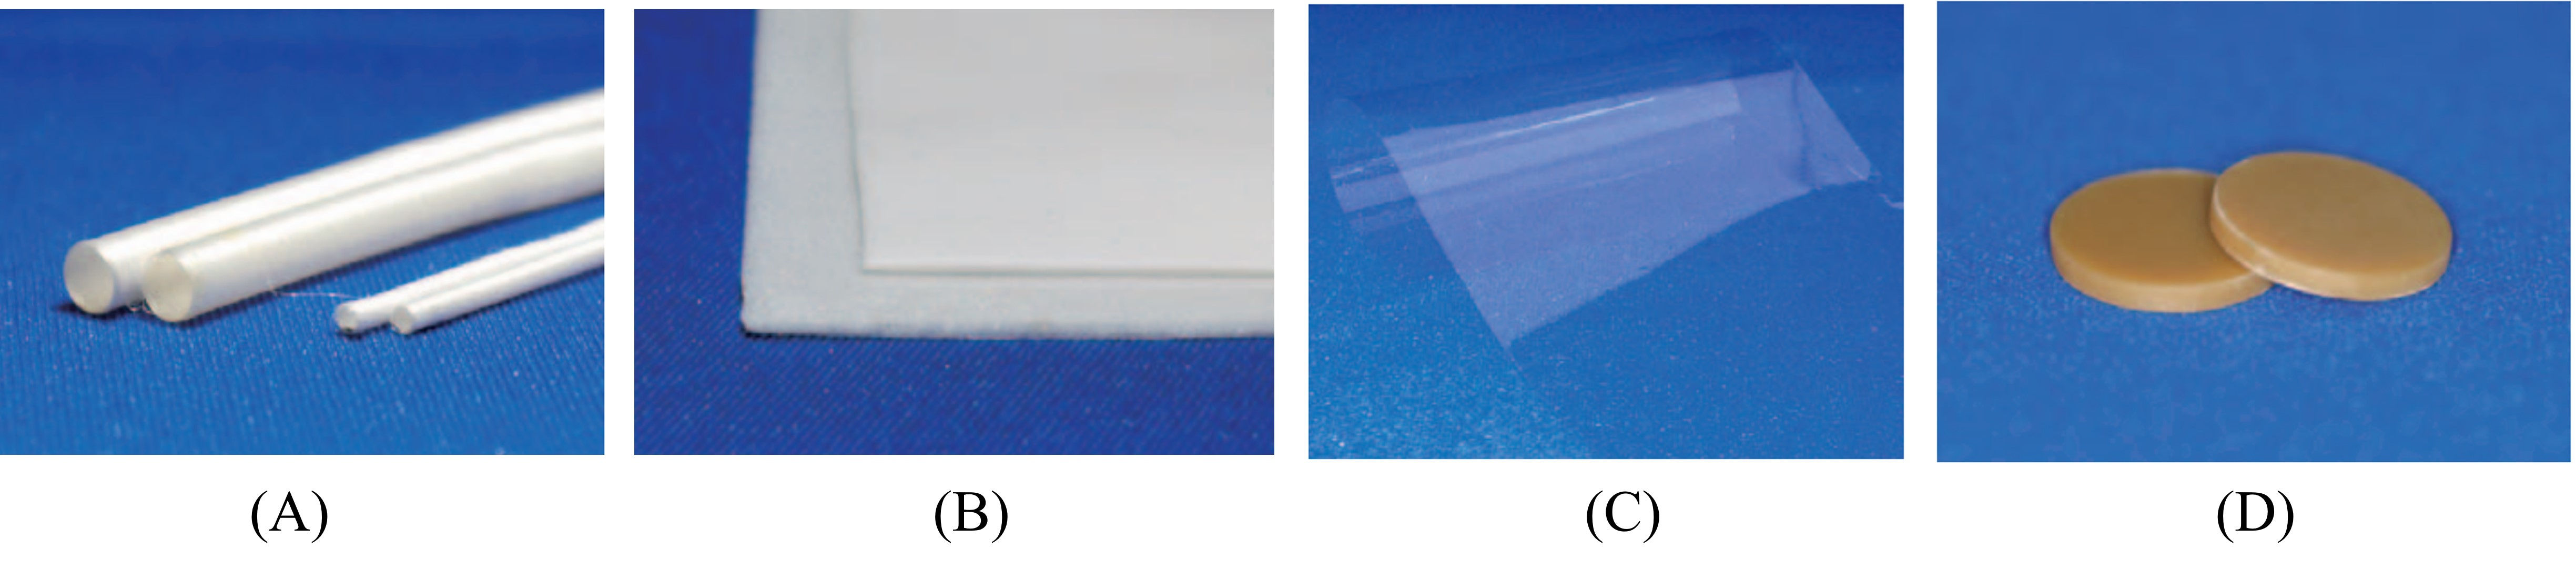
\includegraphics[width=\linewidth]{silk_device.jpg}
			\caption{衣服以外のシルクの利用例\cite{農研機構}。(A)人工血管、(B)シルクスポンジ、(C)フィルム、
			(D)電子回路基板。}
			\label{silk_device}
		\end{figure}
		\newpage
		\subsection{シルクの構造}
		図\ref{fibroin}(a)の様にシルクはフィブロインとセリシンで構成されている。
		シルクを構成する一つの蛋白質であるフィブロインは図\ref{fibroin}(b)の様に分子量の異なる3個の分子により
		構成されている。
		分子量 360 kDaのH鎖と
		27 kDaのL鎖がC末端近傍にてジスルフィド結合したヘテロ2量体が、
		P25の1分子とH鎖の6箇所にて水素結合で繋がっている\cite{fibroin_structure}。
		H鎖は周期構造\cite{H鎖の周期構造}をとる結晶領域とそれを繋ぐ非晶領域が存在する。
		H鎖一本において11個の結晶領域が存在し、
		図\ref{fibroin}(c)のようなアミノ酸配列である。
		結晶領域は最安定状態では逆平行$\beta$シート構造であり、
		結晶構造は単斜晶系をとる\cite{fibroinの結晶構造,marshモデル}。
		これをsilk IIと呼ぶ。
		準安定状態で$\alpha$ helix構造をとり結晶構造は斜方晶系をとる\cite{fibroinの結晶構造,fibroin_準安定状態}。
		これをsilk Iと呼ぶ。図\ref{silk_結晶}の様に加熱や延伸によりsilk Iはsilk IIへ転移する。
		また、薄膜の気液界面にてthreefoldヘリックスを形成し、silk IIIと呼ぶ\cite{silk_III}。

		シルクにおけるセリシンは、図\ref{fibroin}(A)の通りフィブロインを囲む形に存在している。
		しかし、溶解性においては単一の蛋白質ではなく、4種類に分けられる\cite{セリシン構造}。
		表面に分布するセリシンが最も溶解性が高く、内側に進むにつれて溶解性が低くなる。
		溶解性が高い順にsericin I, II, III, IVと呼ばれている\cite{セリシンの微細構造}。

		シルクの構造研究はセリシンが結晶構造を取らないためシルクのフィブロイン構造を指す場合が
		多い。蚕体内の中部紡糸線ではフィブロインとセリシンは液状である。
		これを乾燥させて固体化させるとsilk I 型になる。
		前部紡糸線で液晶化し\cite{絹糸_液晶}、蚕の8の字首振り運動により、前部紡糸線の紡糸菅にて
		延伸され繊維化する。
		繊維化後の状態をsilk IIと呼ぶ。silk IIは延伸されているため配向した
		逆平行$\beta$シートが形成されている。シルクの二次元XRDは図\ref{silk_fiber_debai}の通りであり、デバイシェラー環から
		配向による異方性が伺える\cite{yoshioka2016molecular}。

		シルクの構造はMarshらによって逆平行$\beta$シートのモデルが提案され長く採用されてきた\cite{marshモデル}。
		しかしそのモデルのみだとX線回折像を説明しきれない箇所があるとされている。
		AsakuraらはNMRを用いて構造解析を行い、シルクは分子間間隔の異なる2種類の
		逆平行$\beta$シート構造と歪んだ$\beta$ターン構造で構成されていると主張している\cite{朝倉NMR}。
		また、彼らはsilk I型は$\alpha$ヘリックスではなく
		$\beta$ターンと主張している\cite{asakura_silk1_1,asakura_silk1_2,asakura_silk1_3}。
		\begin{figure}[H]
			\centering
			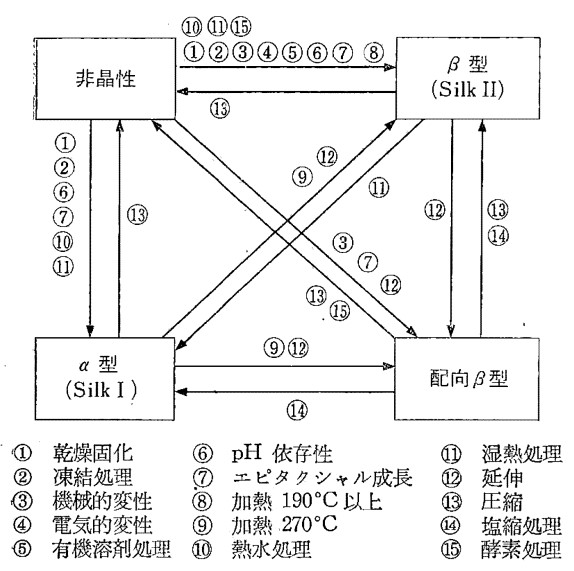
\includegraphics[scale=0.55]{silk_結晶.jpg}
			\caption{シルクフィブロインの構造転移\cite{馬越淳1985絹の結晶化と液晶}}
			\label{silk_結晶}
		\end{figure}
		\newpage
		\begin{figure}[h]
			\centering
			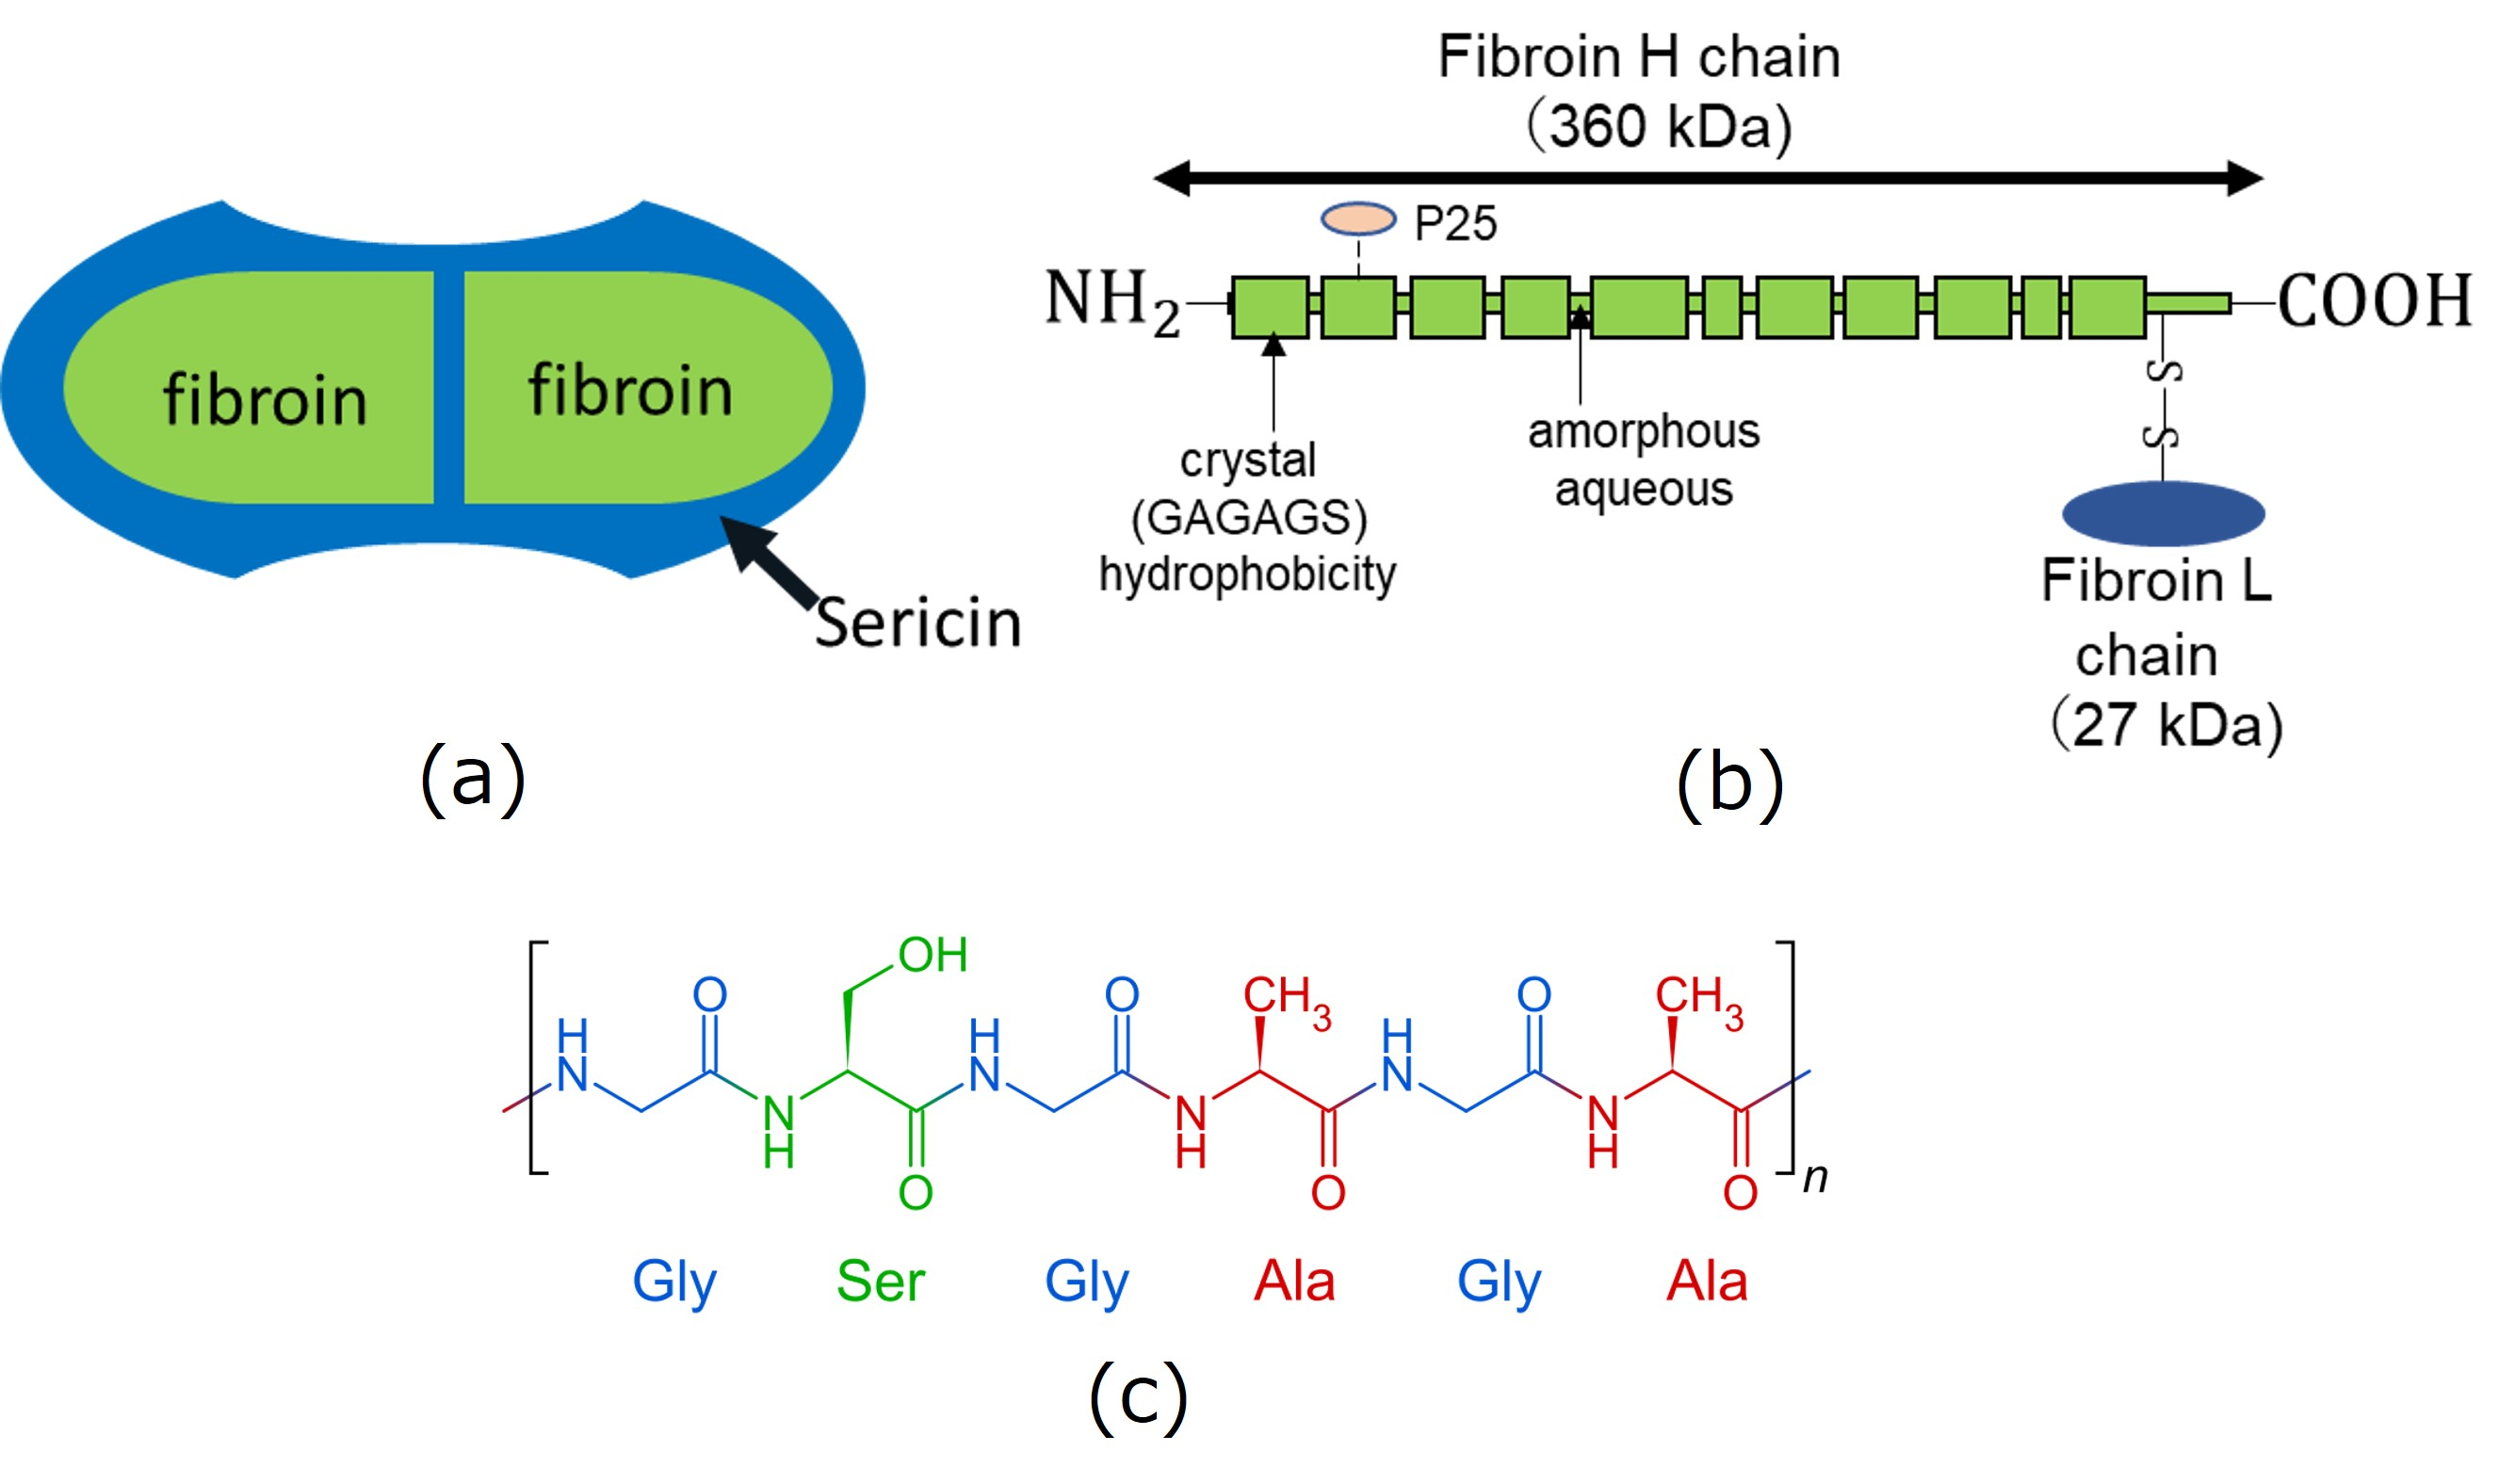
\includegraphics[width=\linewidth]{fibroin_structure.jpg}
			\caption{シルクの構造。(a) シルク1本の構造, (b) フィブロインにおけるH鎖とL鎖の関係, 
			(c) H鎖周期構造におけるアミノ酸配列。}
			\label{fibroin}
		\end{figure}
		\begin{figure}[H]
			\centering
			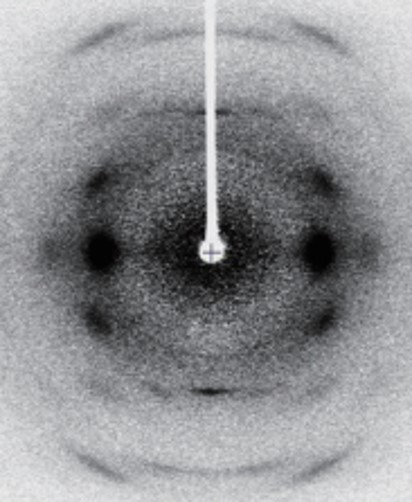
\includegraphics[scale=0.8]{silk_fiber_デバイ.jpg}
			\caption{シルクの2次元XRD\cite{yoshioka2016molecular}。左下の数字はHermanの配向係数。}
			\label{silk_fiber_debai}
		\end{figure}
		\newpage
		\begin{figure}[h]
			\centering
			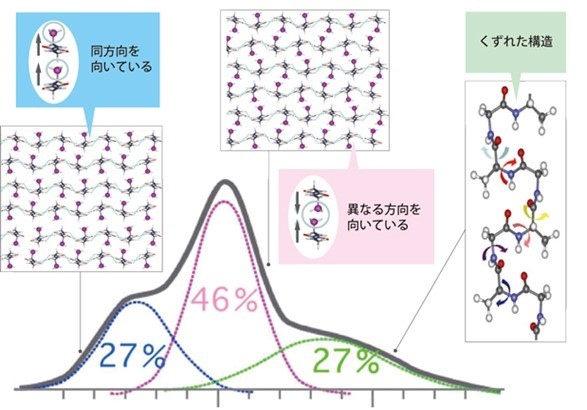
\includegraphics[scale=0.3]{NMR_silk_II.jpg}
			\caption{NMRによるSilk IIの構造解析\cite{朝倉_NMR_研究室,asakura_silk2}}
		\end{figure}
		\newpage
		\section{生体材料の圧電性}
			生体材料における最初の圧電性の報告は、1941年に報告されたMartinによる羊毛を用いた検証とされる。
			羊毛を並べて糊を用いて束にする。束を輪切りにして、断面に力を加えると1 V発生したと報告している。
			同時に焦電性の検証もしており、液体窒素に漬けて温度を下げると約10 Vの
			電圧が発生したと報告している\cite{martin1941}。

			最初に研究が活発になった自然由来の材料として木材が挙げられる。Shubnikovによってその圧電性の予測がされた。
			また、非晶質内で結晶粒子が配向している系をpiezoelectric textureと呼んだ\cite{shubnikov1946}。
			Bazhenov と Konstantinovaによって木材の圧電性の実験が行われた\cite{bazhenov1950}。
			その後、Fukadaによって木材のずり圧電効果の正圧電性と逆圧電性の実験が成功し、
			同時に熱力学的証明を行った\cite{fukada_wood}。
			その後、様々な種類の木材における圧電性など詳細な研究が行われた。その結果、
			木材の対称性は斜方晶系$D_2(222)$に属し、$d_{36}$が有限な値を持ち、$|d_{14}|>|d_{36}|$
			であると示された\cite{平井_木材}。

			蛋白質はアミノ酸が図\ref{アルファヘリックス}(A)の様なペプチド結合(CONH)にて結合した構造を持ち、
			ポリペプチドとも呼ばれる。自然由来の材料、合成材料のどちらにおいても
			ポリペプチド化合物における圧電性の研究が行われてきた。
			自然由来の材料ではコラーゲン\cite{fukada_コラーゲン}、絹\cite{fukada_silk_fiber}、DNA\cite{DNA_圧電性}、皮膚\cite{皮膚_圧電性}、
			骨\cite{hoda_bone_1953,fukada_bone}、腱\cite{fukada_コラーゲン}、
			血管壁\cite{動脈_圧電性}、筋肉\cite{筋肉_圧電性}、貝殻\cite{貝_強誘電性_圧電性}
			においてずりの圧電性があると証明された。
			また、動脈\cite{動脈_強誘電性}や貝\cite{貝_強誘電性_圧電性}には圧電性だけでなく、強誘電性も確認されている。
			合成材料においてはpoly-L-alanine, poly-$\gamma$-methyl-L-glutamate, poly-$\gamma$-benzyl-L-glutamate
			などにおいてもずり圧電が確認されている\cite{合成キラル高分子の圧電性}。

			ずり圧電は高分子における不斉炭素が試料の非対称性に寄与している。
			不斉炭素原子にはL体とD体が存在し、その両方が存在するラセミ体などの材料は統計的鏡映対称性が存在するため、
			ずりの圧電性は生まれない。
			生物を構成するアミノ酸はL体しか存在せず、生物由来の糖はD体のみしか存在しない。
			これを生命のホモキラリティと呼ぶ。
			このようにL体もしくはD体のみ存在する場合、ずりの圧電性が生まれる。
			ずりの圧電性である$d_{14}$の符号はL体で構成されている材料においては負であり、
			D体で構成されている材料は正となる。分子の構造が$\alpha$ヘリックス、
			もしくは引き延ばされた$\beta$型分子のどちらにおいても成立する。
			ただし、$\alpha$ヘリックスは双極子の向きが揃っているため、
			分子の歪みにより大きな分極が発生する可能性があり、圧電性においては
			実験及び理論においても研究が進んでいる。
			\begin{figure}[h]
				\centering
				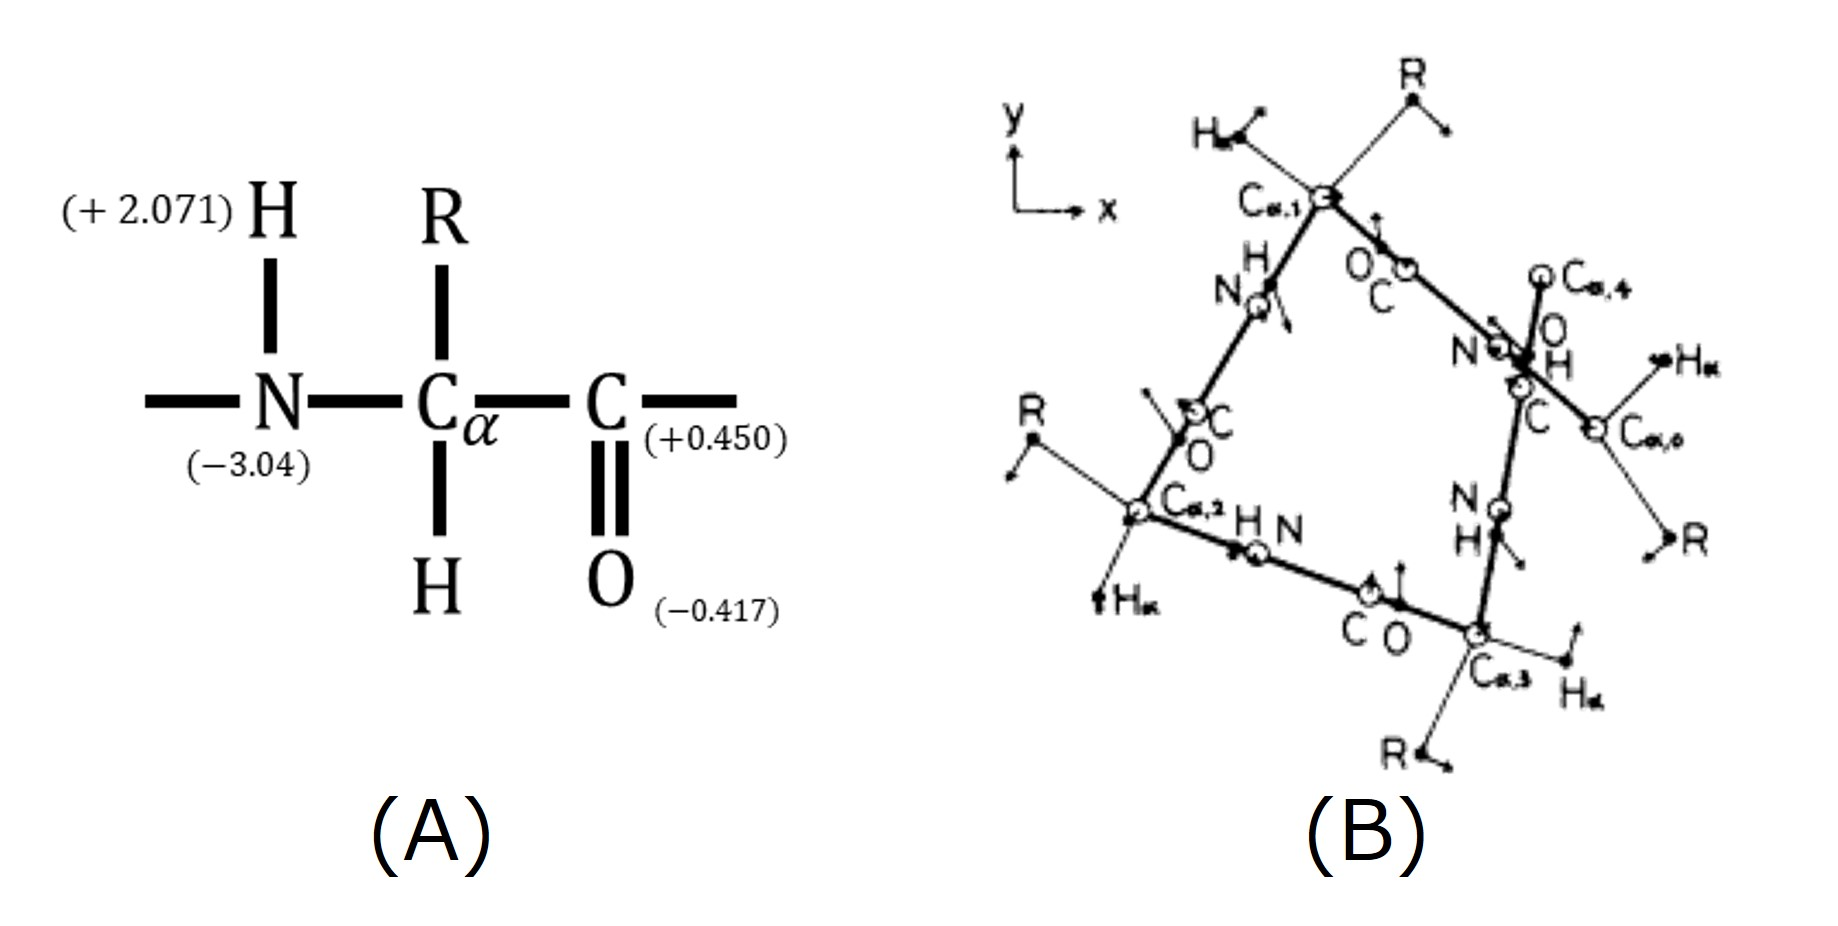
\includegraphics[scale=0.8]{アルファヘリックス_CONH.jpg}
				\caption{ペプチド結合と$\alpha$ヘリックス\cite{CONH_theory}。
				(A) ペプチド結合、(B) $\alpha$ヘリックス内のCONH双極子の内部回転。}
				\label{アルファヘリックス}
			\end{figure}
			ポリペプチドの$\alpha$ヘリックスの圧電性は分子格子力学を用いて計算されている\cite{CONH_theory}。
			ヘリックス骨格の圧電率は$6.3$ pC/Nと報告されており、結晶化度を考慮した
			PBLGの実験値と一致している。
			\subsection{ずりの圧電性を利用したデバイス}
			$\alpha$ヘリックスの圧電性はCONH内部の双極子回転で生じるが、
			最適化された構造の材料としてL体のポリ乳酸がPLLAが挙げられる。
			PLLAは植物由来の合成材料であり、生分解性が高い。
			また、ポリフッ化ビニリデン(PVDF)に匹敵する圧電性を有し、
			加工が容易であり、焦電性が存在せず圧力以外のセンシングを排除できるため
			工業的に注目されている。特に圧電体でありながら焦電性を有さないという点においては
			キネティック系のHMIへの応用として非常に有利である。
			フィルム状のPLLAを利用したデバイスとして図\ref{リーフグリップリモコン}
			の様なリーフグリップリモコンがある\cite{赤本,村田製作所_PLLA}。PLLAの変形から
			デバイスの曲げとねじれの検知が行う。
			\begin{figure}[h]
				\centering
				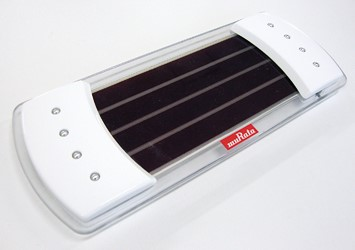
\includegraphics[scale=0.9]{リーフグリップリモコン.jpg}
				\caption{PLLAのずり圧電を利用したリーフグリップリモコン\cite{村田製作所_PLLA}}
				\label{リーフグリップリモコン}
			\end{figure}
			\\
			また、PLLAをfiber状に加工してデバイスに組み込んだ例も報告されている。
			図\ref{PLLA_fiber_device}(A)はPLLAをfiber状からバネ型に加工し、電極を載せたデバイスである。
			バネの伸縮に応じた電圧が計測されている\cite{plla_バネ}。また、図\ref{PLLA_fiber_device}(B)はfiber状のPLLAを
			組み紐に組み込み、ファッショナブルな身体計測デバイスを作製し、脈波などの身体情報を入手した
			と報告している\cite{組み紐_plla}。
			\begin{figure}[H]
				\centering
				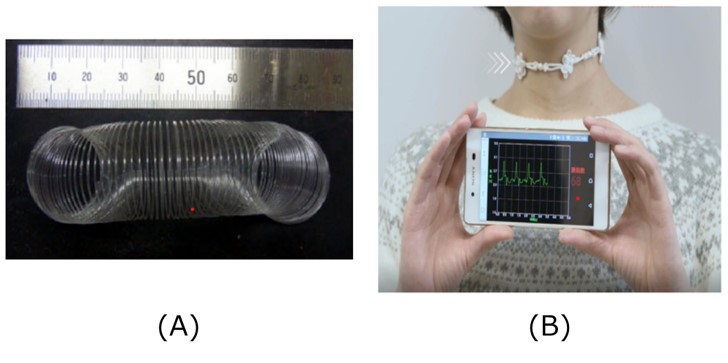
\includegraphics[scale=0.9]{plla_fiber_device.jpg}
				\caption{PLLAをファイバー状に加工してデバイスに組み込んだ事例。
				(A)PLLAをバネ上に加工し振動デバイスを作製\cite{plla_バネ}、(B)PLLAを利用した組み紐型、身体情報計測デバイス\cite{組み紐_plla}}
				\label{PLLA_fiber_device}
			\end{figure}
			\newpage
		\subsection{シルクにおける圧電性}
			シルクの圧電性に関して初めて言及したのはHarveyとされている\cite{Harvey}。
			ただし、定量的な測定などが行われたのではなく、その可能性に言及されたのみに留まる。
			初めて定量的に評価を行ったのはFukadaである\cite{fukada_silk_fiber}。
			乾燥させたシルクを圧縮させて45°カットで切り出し、圧電性を評価した。
			$d$定数がおおよそ1 pC/N程度と報告した。
			ただし、精度に問題があり「おおよそ」と表現されている。
			また、シルクに含まれるセリシンの除去を行うと圧電性の向上が期待できるとも述べられた。
			その後、Yucelらによってシルクのセリシンを除去しフィブロインのキャストフィルムを作製して
			圧電性の報告がされた\cite{fibroin_cast_film_piezo}。
			図\ref{silk_fibroin_cast_装置}の(A)の様に190℃のヒートブロックを
			局所的に試料を温めながら、試料をなぞる様に移動させ、力を加えて延伸する。
			硬くて脆いという特徴があるフィブロインのキャストフィルムだが2.7倍まで延伸したと報告されている。
			図\ref{silk_fibroin_cast_装置}(B)の動的粘弾性装置(Dynamic Mechanical Analysis: DMA)
			を利用してずり圧電の圧電性を評価した。延伸倍率と圧電定数$d_{14}$の関係は図\ref{cast_film_data}(A)
			の通りである。試料の切り出しの角度と圧電定数$d_{14}$の関係は図\ref{cast_film_data}(B)の通りである。
			ずり圧電の特徴である角度依存性が確認出来る。
			\begin{figure}[h]
				\centering
				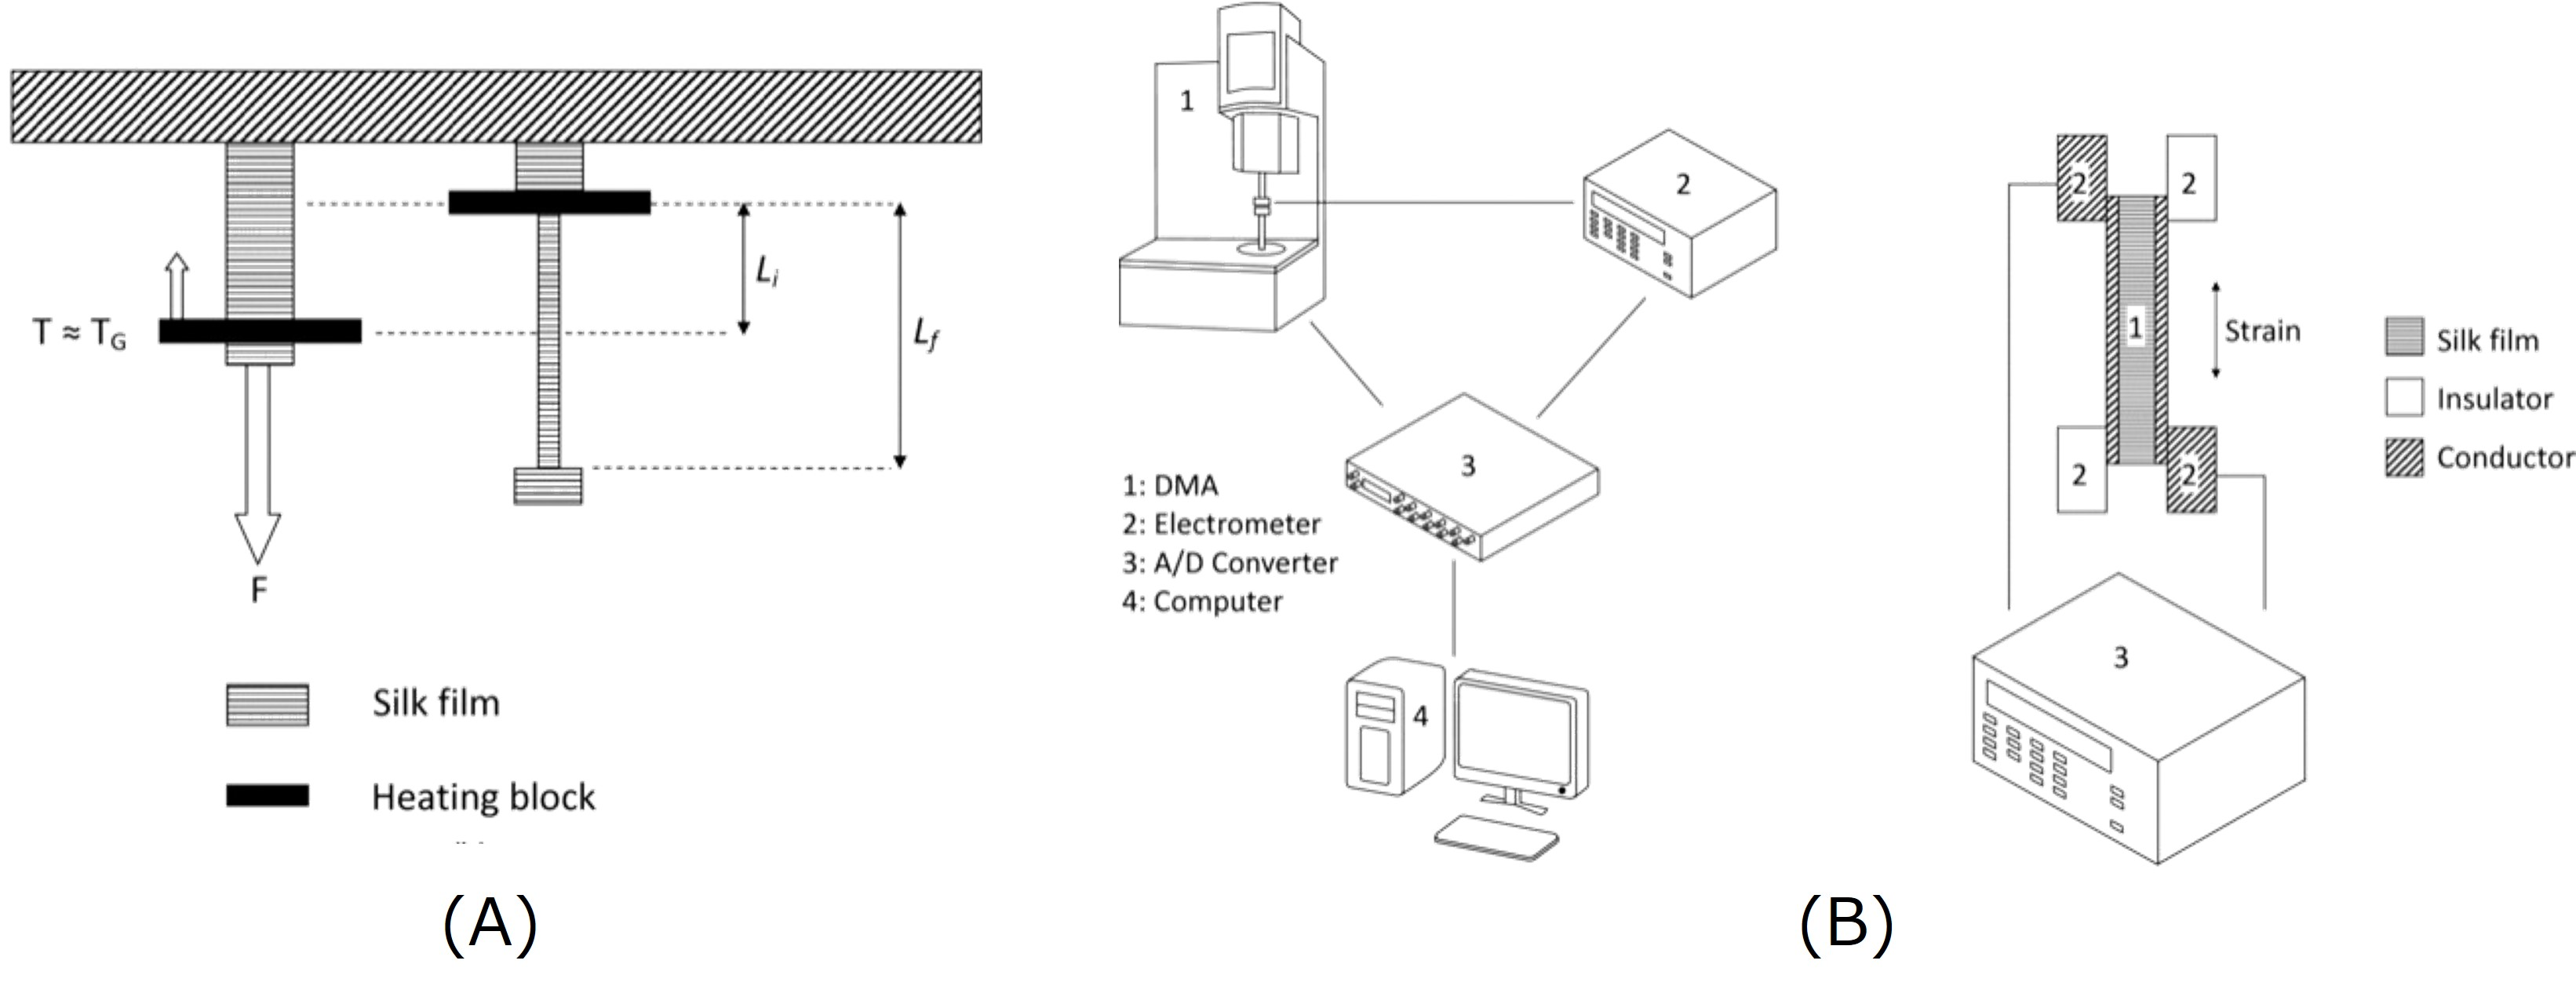
\includegraphics[scale=0.6]{fibroin_piezo_装置.jpg}
				\caption{Fibroin cast filmの延伸と測定装置\cite{fibroin_cast_film_piezo}。
				(A) 延伸の様子、(B) DMA装置を加工したずり圧電の測定装置。}
				\label{silk_fibroin_cast_装置}
			\end{figure}
			\begin{figure}[H]
				\centering
				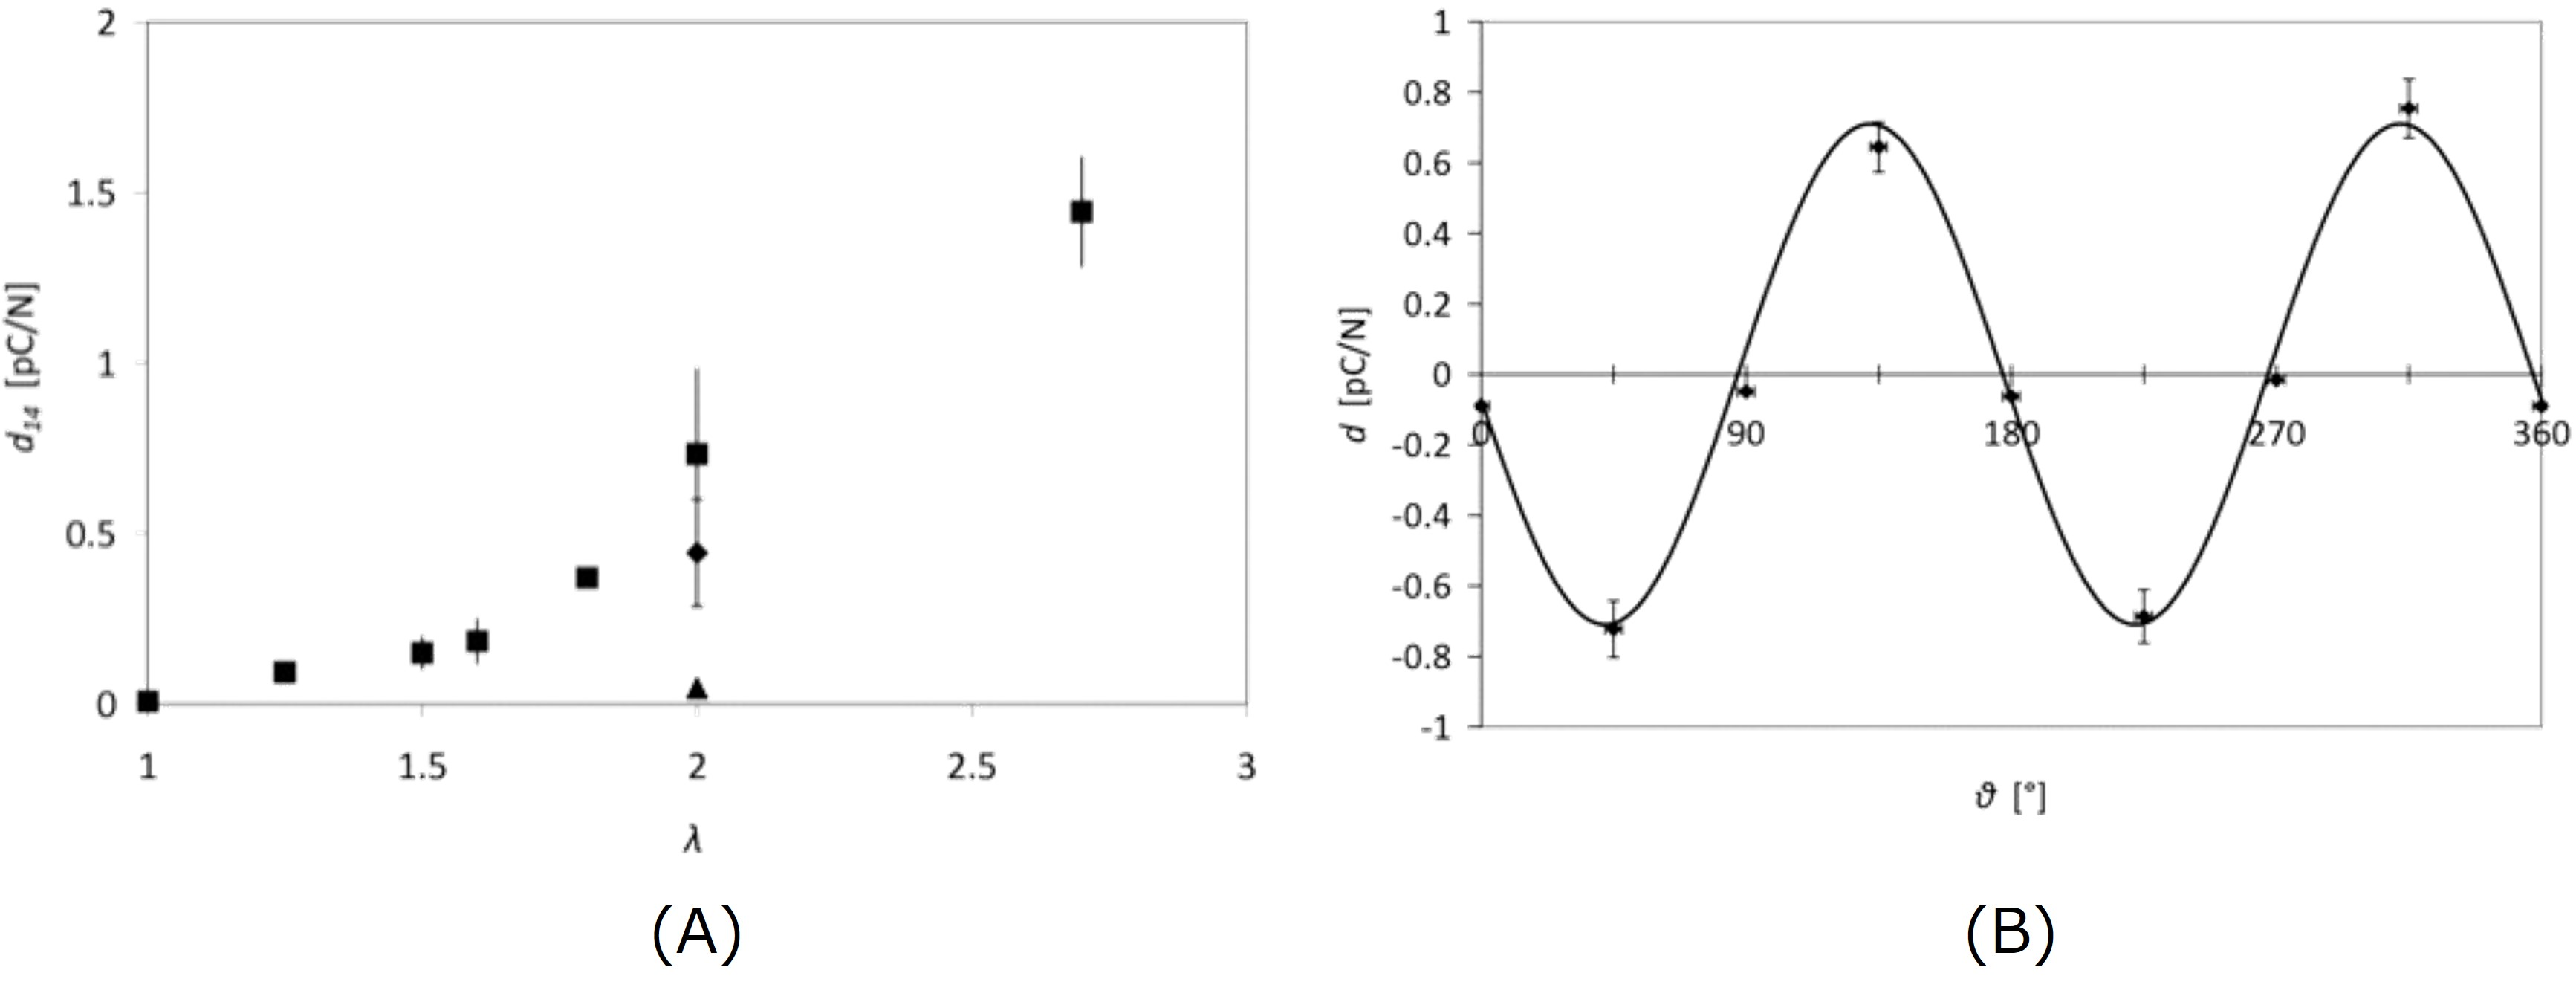
\includegraphics[scale=0.6]{cast_film_piezo_data.jpg}
				\caption{Fibroin cast film における圧電性\cite{fibroin_cast_film_piezo}。
				(A) 延伸倍率と$d_{14}$定数の関係、(B) $d_{14}$定数の角度依存性。}
				\label{cast_film_data}
			\end{figure}
			\newpage
			また、FTIRやXRDのデータを合わせて検証した結果、
			図\ref{orientation_beta_sheet_piezo}のように
			配向性と逆平行$\beta$ sheet の含有量の両方を高める
			と圧電性が向上すると述べている。
			\begin{figure}[h]
				\centering
				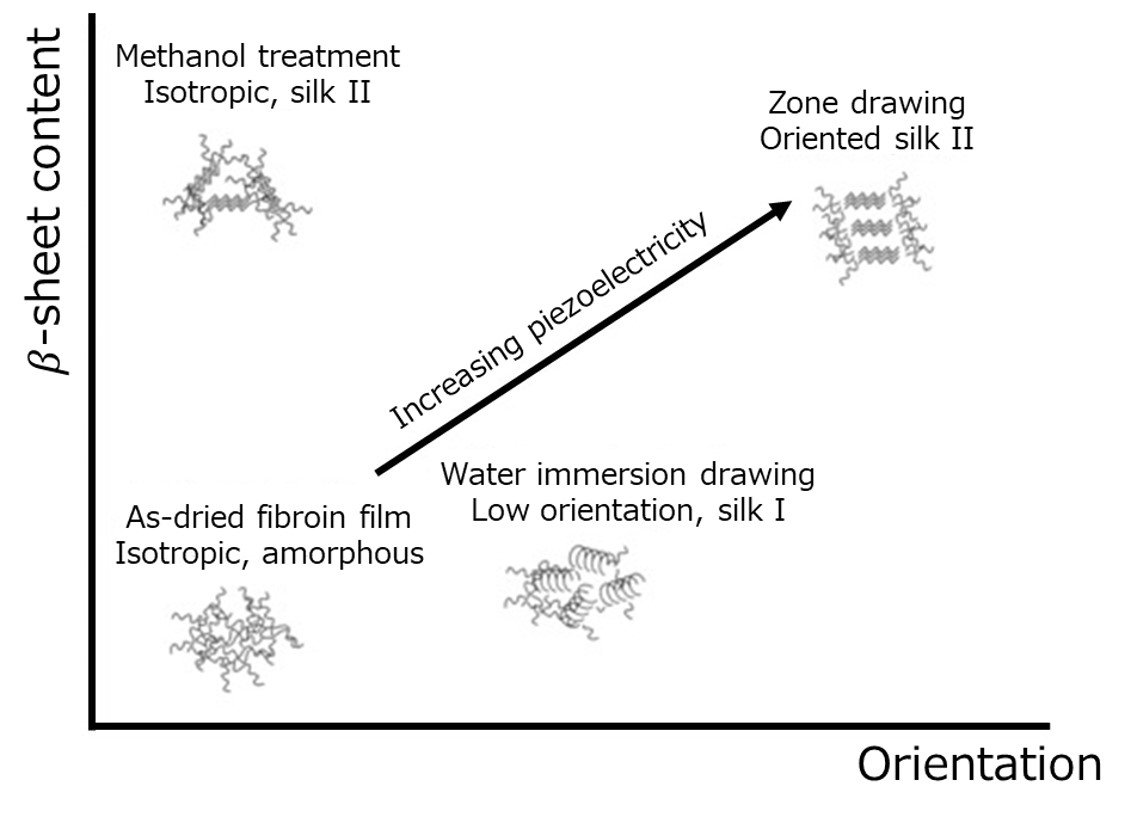
\includegraphics[scale=0.6]{orientation_beta_sheet_piezo.jpg}
				\caption{配向性、逆平行$\beta$ sheetの含有量と圧電性の関係\cite{fibroin_cast_film_piezo}}
				\label{orientation_beta_sheet_piezo}
			\end{figure}
			\\
			
			Fiber状で作製し、圧電性を検証した事例としてエレクトロスピニング法(電界紡糸法)による報告がある\cite{エレクトロスパン}。
			エレクトロスピニング法(電界紡糸法)とは、
			糸ノズル内のポリマー溶液に高電圧を加えて、ナノファイバーを生成する製法である。
			エレクトロスピニング法を活用してFibroin溶液からFibroin nano fiberを作製し、その圧電性を
			DMA装置やPFMを用いて報告している。
			\begin{figure}[h]
				\centering
				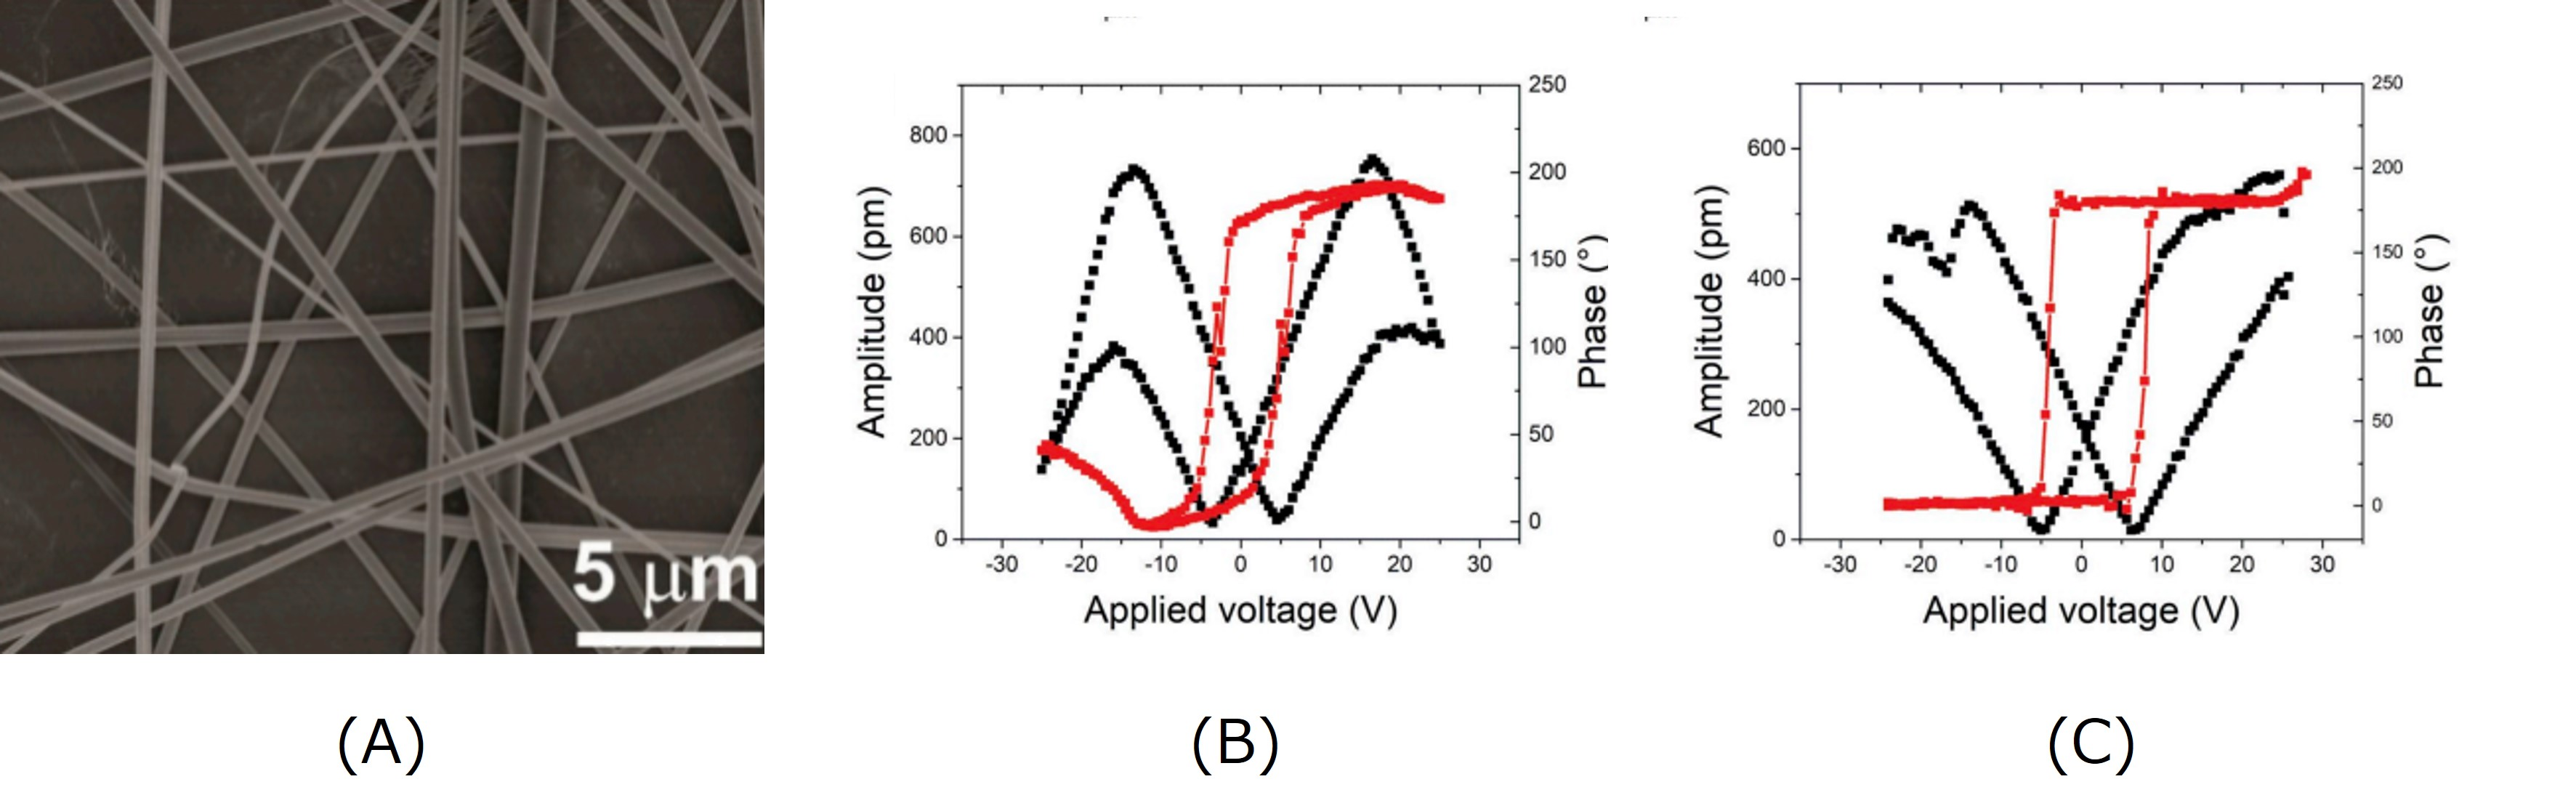
\includegraphics[scale=1]{electrospun_data.jpg}
				\caption{エレクトロスピニング法によるFibroin nano fiber\cite{エレクトロスパン}。
				(A)SEM像、(B)PFMを用いた圧電バタフライ曲線}
				\label{electrospun}
			\end{figure}
			\newpage
			シルクフィブロインの圧電性が低いため、ナノ粒子の強誘電体を混ぜて圧電性を向上させる方法がある。
			また、圧電性を向上させるのと同時にデバイスに利用する例が頻繁に報告されている。
			しかし、圧電性能がナノ粒子の分散の程度に大きく依存し、社会実装には至っていない。

			ペロブスカイト型の圧電体としてチタン酸ジルコン鉛(PZT)が有名だが、鉛を含むため毒性が高い。
			よって、PZT以外のペロブスカイト型の圧電体であるBaTiO$_3$、ZnSO$_4$などのナノ粒子を
			シルクフィブロインに混ぜ生体適合性を担保しつつ圧電性を向上させ、
			人の動きによって発電するワイヤー状のデバイスを開発したという報告されている\cite{kim2015silk}。
			他にも酸化亜鉛のナノロッドをフィブロイン膜に作製し、e-skinとして実装した報告もあるが
			生体適合性の課題は残されたままである\cite{gogurla2020self}。
			
			蚕のシルクではないがクモの糸もフィブロインである。クモの糸のフィブロインの圧電性を利用したエナジーハーベスター
			も報告されている。電極の上にクモの糸を並べて素子を作製し、
			整流しコンデンサーに蓄えたと報告している\cite{karan2018nature}。

		\section{研究の目的}
		環境に優しい機能性材料に注目が集まっているため、
		生体適合性、生分解性、圧電性を有するシルクも期待されている。
		しかしながら報告されているシルクを圧縮して作製されたシルクフィルムは精度の良い定量的な評価に至っていない。
		また、シルクの一部を利用したフィブロインのキャストフィルムによる圧電性評価の報告は試料に直接的に
		力を加えて計測する方法であり、圧電共鳴法程、正確ではない。
		また、材料を溶解させて試料を作製するキャストフィルムはシルクの高い配向性を利用していない。
		
		本研究では、シルクの高い配向性を利用し熱プレスを用いてシルクフィルムを作製した。
		また、得られた試料に対し、圧電共鳴法を用いて定量的かつ高精度に圧電性、誘電性、機械特性を
		評価することを目的とした。
	\chapter{原理}
		\section{圧電性}
		\subsection{圧電基本式}
		圧電体には正圧電効果と逆圧電効果という性質が存在する。
		生じた歪みに対して、応力と電場の寄与がある。
		さらに生じた電束密度に対しても応力と電場の二つの寄与がある。
		これらを式にまとめると
				\begin{eqnarray}
					\begin{cases}
						\delta S=\frac{\partial S}{\partial T}\delta T + \frac{\partial S}{\partial E} \delta E 
						= s^{E}\delta T+d \delta E & \\
						\delta D=\frac{\partial D}{\partial T}\delta T + \frac{\partial D}{\partial E}\delta E 
						= d \delta T+\varepsilon^T \delta E  &
					\end{cases}
					\label{圧電d形式1}
				\end{eqnarray}
			となる。実際の試料は1軸方向、2軸方向、3軸方向のみだけでなく、
			せん断歪みを考慮する必要があり、テンソル形式で記述される。
			ここで、$\delta S\rightarrow S, \delta T\rightarrow T,
			\delta E\rightarrow E, \delta D\rightarrow D$とし、テンソル行列を$\left[ \right]$で表すと
			式\eqref{圧電d形式1}は
			\begin{equation}
				\begin{cases}
					\left[S\right]=\left[s^E\right]\left[T\right]+\left[d_t\right]\left[E\right]& \\
					\left[D\right]=\left[d\right]\left[T\right]+\left[\varepsilon^T\right]\left[E\right]
				\end{cases}
				\label{圧電d形式2}
			\end{equation}
			となり、これを圧電$d$形式と呼ぶ。
			式\eqref{圧電d形式2}をテンソルの要素も含めて記述すると
			\begin{equation}
				\begin{cases}
				\left(
				\begin{array}{c}
					S_1 \\
					S_2 \\
					S_3 \\
					S_4 \\
					S_5 \\
					S_6 
				\end{array}
				\right)=\left(
				\begin{array}{cccccc}
				s^E_{11} & s^E_{12} & s^E_{13} & s^E_{14} & s^E_{15} & s^E_{16} \\
				s^E_{21} & s^E_{22} & s^E_{23} & s^E_{24} & s^E_{25} & s^E_{26} \\
				s^E_{31} & s^E_{32} & s^E_{33} & s^E_{34} & s^E_{35} & s^E_{36} \\
				s^E_{41} & s^E_{42} & s^E_{43} & s^E_{44} & s^E_{45} & s^E_{46} \\
				s^E_{51} & s^E_{52} & s^E_{53} & s^E_{54} & s^E_{55} & s^E_{56} \\
				s^E_{61} & s^E_{62} & s^E_{63} & s^E_{64} & s^E_{65} & s^E_{66} \\
				\end{array}
				\right)
				\left(
				\begin{array}{c}
					T_1 \\
					T_2 \\
					T_3 \\
					T_4 \\
					T_5 \\
					T_6 
				\end{array}
				\right)+
				\left(
				\begin{array}{ccc}
					d_{11} & d_{21}	& d_{31} \\
					d_{12} & d_{22}	& d_{32} \\
					d_{13} & d_{32}	& d_{33} \\
					d_{14} & d_{42} & d_{34} \\
					d_{15} & d_{52} & d_{35} \\
					d_{16} & d_{62}	& d_{36}
				\end{array}
				\right)
				\left(
				\begin{array}{c}
					E_1 \\
					E_2 \\
					E_3 \\
				\end{array}
				\right) & \\
				\left(
				\begin{array}{c}
					D_1 \\
					D_2 \\
					D_3
				\end{array}\right)=\left(
				\begin{array}{cccccc}
					d_{11} & d_{12} & d_{13} & d_{14} & d_{15} & d_{16} \\
					d_{21} & d_{22} & d_{23} & d_{24} & d_{25} & d_{26} \\
					d_{31} & d_{32} & d_{33} & d_{34} & d_{35} & d_{36}
				\end{array}\right)
				\left(
				\begin{array}{c}
					T_1 \\
					T_2 \\
					T_3 \\
					T_4 \\
					T_5 \\
					T_6 
				\end{array}
				\right)+\left(
				\begin{array}{ccc}
					\varepsilon^T_{11}&0&0 \\
					0&\varepsilon^T_{11}&0 \\
					0&0&\varepsilon^T_{33}
				\end{array}\right)
				\left(
				\begin{array}{c}
					E_1 \\
					E_2 \\
					E_3 \\
				\end{array}\right)
				\end{cases}
				\label{圧電d形式_テンソル}
			\end{equation}
			となる。式\eqref{圧電d形式2}を式変形すると
			\begin{equation}
				\begin{cases}
				\left[T\right]=\left[c^E\right]\left[S\right]-\left[e_t\right]\left[E\right] & \\
				\left[D\right]=\left[e\right]\left[S\right]+\left[\varepsilon^S\right]\left[E\right]
				\end{cases}
				\label{圧電e形式}
			\end{equation}
			\begin{equation}
				\begin{cases}
					\left[S\right]=\left[s^D\right]\left[T\right]-\left[g_t\right]\left[D\right] & \\
					\left[E\right]=-\left[g\right]\left[T\right]+\left[\beta^T\right]\left[D\right]
				\end{cases}
				\label{圧電g形式}
			\end{equation}
			\begin{equation}
				\begin{cases}
					\left[T\right]=\left[c^D\right]\left[S\right]-\left[h_t\right]\left[D\right] & \\
					\left[E\right]=-\left[h\right]\left[S\right]+\left[\beta^s\right]\left[D\right]
				\end{cases}
				\label{圧電h形式}
			\end{equation}
			の三式を導け、それぞれ式\eqref{圧電e形式}を圧電$e$形式, 
			式\eqref{圧電g形式}を圧電$g$形式, 式\eqref{圧電h形式}を圧電$h$形式と呼ぶ。応力$T$, 電場$E$, 歪み$S$, 電束密度$D$の係数である$[d],[e],[g],[h]$ではそれぞれ、
			\begin{equation}
				d_{ij}=\left(\frac{\partial D_i}{\partial T_j}\right)_E=\left(\frac{\partial S_j}{\partial E_i}\right)_T
			\end{equation}
			\begin{equation}
				e_{ij}=\left(\frac{\partial D_i}{\partial S_j}\right)_E=-\left(\frac{\partial T_j}{\partial E_i}\right)_S
			\end{equation} 
			\begin{equation}
				g_{ij}=-\left(\frac{\partial E_i}{\partial T_j}\right)_D=\left(\frac{\partial S_j}{\partial D_i}\right)_T
			\end{equation}
			\begin{equation}
				h_{ij}=-\left(\frac{\partial E_i}{\partial S_j}\right)_D=-\left(\frac{\partial T_j}{\partial D_i}\right)_S
			\end{equation}
			で定義される。また、それぞれの圧電定数間には弾性コンプライアンス$s$、
			誘電率$\varepsilon$を介して以下の関係がある。
			\begin{equation}
				d = e s
				\label{e_to_d}
			\end{equation}
			\begin{equation}
				g = h s
			\end{equation}
			\begin{equation}
				d = \varepsilon g
			\end{equation}
			\begin{equation}
				e = \varepsilon h
			\end{equation}
			$d, e, g, h$はどれも式\eqref{圧電d形式_テンソル}の様にテンソルで記述される。
			具体的なテンソルの中身は結晶と試料の全体の対称性から決まる。
			結晶が無秩序に存在する場合、分子や結晶の対称性に関係なく圧電性は現れない。
			結晶が無秩序に存在する状態は、$\infty$個の$\infty$回軸がある。
			延伸やポーリングなどの処理により$\infty$回軸を減らす。
			圧電性や焦電性を示すマクロな対称性においては$\infty (C_\infty), \infty$ mm
			($C_{\infty v}$), $\infty 2(D_\infty)$の3群となる。
			シルクフィブロインは$D_\infty$となり圧電$d$テンソルは以下のように決まる。
			\begin{equation}
				\left(
				\begin{array}{cccccc}
					0 & 0 & 0 & d_{14} & 0 & 0 \\
					0 & 0 & 0 & 0 & -d_{14} & 0 \\
					0 & 0 & 0 & 0 & 0 & 0
				\end{array}\right)
			\end{equation}
			\newpage
			\subsection{電気機械結合係数}
			物理変数が異なる系の物理変数を変化させる現象を結合効果という。
			試料に加えられた力や温度によって分極が変化する現象である圧電性、焦電性は結合効果の一つである。
			\begin{figure}[h]
				\centering
				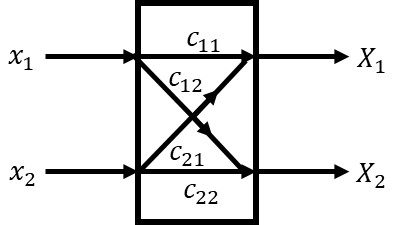
\includegraphics{結合効果.jpg}
				\caption{線形な結合効果\cite{応用物性}}
				\label{結合効果}
			\end{figure}

			図\ref{結合効果}のように2種類の共役な物理変数 ($x_1$, $X_1$),($x_2$, $X_2$)
			について、その間に線形な結合があるとする。
			熱力学ポテンシャルは、一般化したひずみ $x$ を独立変数として
			式\eqref{線形結合効果の熱力学ポテンシャル}のように記述出来る。
			\begin{equation}
				\Phi=\frac{1}{2}c_{11}x_1^2 + c_{12}x_1x_2+\frac{1}{2}c_{22}x_2^2
				\label{線形結合効果の熱力学ポテンシャル}
			\end{equation}
			$x$に共役な物理変数$X$は
			\begin{equation}
				X_1 = \left( \frac{\partial \Phi}{\partial x_1} \right)_{x_2} = c_{11}x_1+c_{12}x_2
			\end{equation}
			\begin{equation}
				X_2 = \left( \frac{\partial \Phi}{\partial x_2} \right)_{x_1} = c_{12}x_1 + c_{22}x_2
			\end{equation}
			となり、係数 $c_{12}$を介して異なる物理変数への結合が起きることが分かる。
			非線形な結合である場合も線形な場合と同様の上式2つで記述できる。
			両方向の結合の係数が等しく、これを相反定理($c_{12}=c_{21}$)という。
			また、異なる系の間におけるエネルギー変換効率として結合系数$k$を式\eqref{結合係数}のように定義する。
			\begin{equation}
				k^2=\frac{c_{12}^2}{c_{11}c_{22}}
				\label{結合係数}
			\end{equation}
			
			例えば共役な変数($x_1$, $X_1$)として応力$T$とひずみ$S$を採用する。
			また、もう一つの共役な物理変数($x_2$, $X_2$)として電場$E$と電束密度$D$を採用する。
			その二つの共役な物理変数を結ぶ結合の係数を$d$とおくとき、熱力学ポテンシャル$\Phi$は以下のように書ける。
			\begin{equation}
				\Phi = \frac{1}{2}s^ET^2 + d T E + \frac{1}{2}\varepsilon^T E^2
			\end{equation}
			一般化した議論と同様に熱力学ポテンシャル$\Phi$から$X_1=S$, $X_2=D$を計算する
			と以下のように圧電$d$形式を入手できる。
			\begin{equation}
				S = \left(\frac{\partial \Phi}{\partial T} \right)_E = s^E T + d E
			\end{equation}
			\begin{equation}
				D=\left(\frac{\partial \Phi}{\partial E}\right)_T = dT+\varepsilon^T E
			\end{equation}
			結合係数$k$は以下のように記述でき、電気的特性と機械的特性の変換であるため電気機械結合係数と呼ばれる。
			\begin{equation}
				k^2 = \frac{d^2}{\varepsilon^Ts^E}
				\label{電気機械結合係数d}
			\end{equation}

			自由境界条件($T=0$)で逆圧電効果を例に単位体積当たりの入力のエネルギーと出力のエネルギーを計算する。
			圧電$d$形式、式\eqref{圧電d形式1}から自由状態($T=0$)において電源から
			\begin{equation}
				D=\varepsilon^T E
			\end{equation}
			という電束密度が供給される。これより、入力された電気エネルギー$U_{in}$は以下のように計算される。
			\begin{equation}
				U_{in} = \int^{D}_0 E dD = \int^{D}_0 \frac{D}{\varepsilon^T} dD  
				= \frac{1}{2}\frac{D^2}{\varepsilon^T}
				= \frac{1}{2}\varepsilon^T E^2 
			\end{equation}
			圧電体においては、入力された電気エネルギー$U_{in}$の一部が機械エネルギーに変換される。
			電場に対するひずみは圧電$d$形式、式\eqref{圧電d形式1}において$T=0$として以下の通りである。
			\begin{equation}
				S = d E
			\end{equation}
			単位体積あたりの機械エネルギーは
			\begin{equation}
				U_{out} = \int^S_0 \frac{S}{s^E} d S = \frac{1}{2} \frac{1}{s^E}S^2 
				= \frac{1}{2}\frac{d^2}{s^E}E^2
			\end{equation}
			となる。よって入力電気エネルギーと出力機械エネルギーの割合は以下のように、式\eqref{電気機械結合係数d}
			と同等の電気機械結合係数を得る。
			\begin{equation}
				k^2 = \frac{\mbox{出力機械的エネルギー}}{\mbox{入力電気的エネルギー}}
				= \frac{U_{out}}{U_{in}} = \frac{\frac{1}{2}\varepsilon^T E^2}{\frac{1}{2}\frac{d^2}{s^E}E^2}
				= \frac{d^2}{\varepsilon^T s^E}
			\end{equation}
			また、正圧電効果も同様に議論でき以下の関係が言える。
			\begin{equation}
				k^2=\frac{\mbox{出力機械的エネルギー}}{\mbox{入力電気的エネルギー}}=
				\frac{\mbox{出力電気的エネルギー}}{\mbox{入力機械的エネルギー}}
				\label{電気機械結合係数の定義}
			\end{equation}
			電気機械結合係数の二乗$k^2$がエネルギーの変換効率となる。
			$1-k^2$は正圧電効果では機械エネルギーが電気エネルギーに
			変換されなかったエネルギーの総エネルギーに対する割合であり、
			逆圧電効果では材料に蓄えられたエネルギーの総エネルギーに対する割合となる。

			また、$1-k^2$は応力$T$を0とした誘電率$\varepsilon^T$と歪み$S$を0としたときの
			誘電率$\varepsilon^S$の比とも解釈される。
			式\eqref{圧電d形式1}の圧電$d$形式の2式目を以下のように応力$T$を求める形に式変形する。			
			\begin{equation}
				T = \frac{D-\varepsilon^T E}{d}
			\end{equation}
			上式を式\eqref{圧電d形式1}の1式目に代入し、電束密度$D$を求める形に変形する。
			この際に式\eqref{電気機械結合係数d}を使用した。
			また、圧電$e$形式である式\eqref{圧電e形式}の2式目と等価となる。
			\begin{equation}
				D = \frac{d}{s^E}S + \varepsilon^T\left(1-k^2\right)E
				  = e S + \varepsilon^S E
			\end{equation}
			上式において発生する歪み$S$を0としたとき、以下の関係が導ける。
			\begin{equation}
				\frac{\varepsilon^S}{\varepsilon^T}=1-k^2
			\end{equation}
			インピーダンスアナライザなどを用いて容量を計測し、印加電圧の周波数を変動させながら
			圧電共鳴を計測したとする。圧電共鳴が発生する周波数$f_R$より低周波側は
			自由端条件であり、高周波側は固定端条件となる。
			自由端条件は応力$T$を0とした誘電率$\varepsilon^T$、
			固定端条件では歪み$S$を0とした誘電率$\varepsilon^S$が対応する。
			容量から誘電率を計算するが、以下の式では誘電率の比率であるため
			試料寸法の計測エラーが消える。
			\newpage
		\section{誘電性}
		電場が印加されると分極を生じる性質を誘電性といい、誘電性を有する物質を誘電体と呼ぶ。
		また、このとき生じる分極を誘電分極と呼ぶ。
		圧電体は誘電体に内包される関係である。
		中心対称性がない誘電体は圧電性を示す誘電体であり、
		中心対称性が存在する誘電体は圧電性を示さない。
		よって圧電体は誘電体としての特性も有する。
		時間変動する電場に対する誘電体の特性を紹介する。
			\subsection{誘電応答における時間的な遅れ}
			時間とともに変動する電場に対して、誘電応答は時間的に遅れて生じる。
			これを誘電緩和現象という。
			電場が角周波数$\omega$で正弦波的に変動すると式\eqref{E(t)}の様に表現される。
			\begin{equation}
				E(t)=E_0 e^{i\omega t}
				\label{E(t)}
			\end{equation}
			電束密度は振幅$D_0$、位相が$\delta$遅れた信号として観測されると式\eqref{D(t)}の様に表現される。
			\begin{equation}
				D(t)=D_0 e^{i(\omega t-\delta)}
				\label{D(t)}
			\end{equation}
			誘電率$\varepsilon$は電束密度$D$と電場$E$の比例係数として定義されるため式\eqref{E(t)}と式\eqref{D(t)}
			の比は以下のように計算される。
			\begin{equation}
				\frac{D(t)}{E(t)}=\frac{D_0e^{i(\omega t-\delta)}}{E_0 e^{i\omega t}}
				=\frac{D_0}{E_0}\left(\cos\delta-i\sin\delta\right)=\varepsilon'(\omega)-i\varepsilon''(\omega)
			\end{equation}
			誘電率実部$\varepsilon'$は加えた電場が電気エネルギーとして蓄えられる成分に対応し、貯蔵誘電率とも呼ばれる。
			誘電率虚部$\varepsilon''$は熱エネルギーとなって散逸する成分に対応し、損失誘電率と呼ばれる。
			誘電率実部$\varepsilon'$と誘電率虚部$\varepsilon''$の比は以下の通りであり、損失正接(loss tanget)、
			$\delta$を損失角と呼ぶ。
			\begin{equation}
				\frac{\varepsilon''}{\varepsilon'}=\tan\delta
				\label{tandel}
			\end{equation}
			時間的なずれ($\delta$)の物理的な要因は分極の原因となる電荷の変位や双極子の回転が起こるときに、
			粘性抵抗や質量の効果が働くといった点が挙げられる。その結果、誘電率は測定する周波数に依存して分散現象を示し、
			分極の機構によってさまざまなスペクトルを描く。
			\subsection{誘電性と導電性の関係}
			誘電体は直流におけるインピーダンスの高さから絶縁体の一種とされている。
			しかし交流波においては、周波数が高くなるほどインピーダンスが小さくなり導電性が高くなる。
			電束密度$D$の時間微分は電流密度$J$であり、式\eqref{D(t)}を用いて計算すると以下のようになる。
			\begin{equation}
				J=\frac{\partial D}{\partial t}=i\omega D
				\label{電流密度}
			\end{equation}
			オームの法則は以下の通りである。
			\begin{equation}
				J=\sigma E
				\label{オームの法則}
			\end{equation}
			式\eqref{電流密度}と式\eqref{オームの法則}は等価であるため、
			誘電率の実部$\varepsilon'$虚部$\varepsilon''$と
			導電率の実部$\sigma'$虚部$\sigma''$において
			以下の関係が得られる。
			\begin{equation}
				\sigma'=\omega\varepsilon''
			\end{equation}
			\begin{equation}
				\sigma''=\omega\varepsilon'
			\end{equation}
			\subsection{周波数応答関数とパルス応答関数}
			ステップ状の電場$E_s$を時間$t=0$において印加したときの電束密度の時間変化を$D_s(t)$とする。
			誘電率は以下のように表現され、誘電余効関数と呼ぶ。
			\begin{equation}
				\varepsilon(t)=\frac{D_s(t)}{E_s}
			\end{equation}
			パルス状の$\delta$関数がステップ関数の一回微分であるため、パルス状の電場を印加したときにおける
			誘電率の時間応答関数は以下のように、誘電余効関数の一回微分となる。また、$\varepsilon_p(t)$をパルス応答関数と呼ぶ。
			\begin{equation}
				\varepsilon_p(t)=\frac{d\varepsilon(t)}{dt}
				\label{パルス応答関数}
			\end{equation}
			応答が刺激により生じるという因果性、一定の刺激に対して一定の応答が生じるという定常性、
			複数の刺激に対する応答は、それぞれの刺激に対する応答の和で与えられるという線形生を仮定する。
			任意の電場$E(t)$に対して生じる電束密度$D(t)$はパルス応答関数を用いて以下のように表現される。
			\begin{equation}
				D(t)=\int^{\infty}_0 \varepsilon_p(t_1)E(t-t_1) dt_1
				\label{ボルツマン重ね合わせの原理}
			\end{equation}
			時間$t$に表れる電束密度という応答が時間$t_1$に与えたパルス刺激の応答の重ね合わせになっている。
			これをボルツマン重ね合わせの原理という。正弦波の電場を印加したとして式\eqref{E(t)}を式\eqref{ボルツマン重ね合わせの原理}
			に代入する。
			\begin{equation}
				D(t)=\int^{\infty}_0 \varepsilon_p(t_1)E_0e^{i\omega(t-t_1)}dt_1=E(t)\int^{\infty}_0 \varepsilon_p(t_1)e^{-i\omega t_1}dt_1
			\end{equation}
			誘電率は以下のように計算される。
			\begin{equation}
				\varepsilon(t)=\frac{D(t)}{E(t)}=\int^{\infty}_0 \varepsilon_p(t_1)e^{-i\omega t_1} dt_1
			\end{equation}
			$t_1\rightarrow t$にすると上式の最右辺はフーリエ変換の式となる。
			周波数応答関数とパルス応答関数が互いにフーリエ変換の関係であると分かる。
			\begin{equation}
				\varepsilon(\omega)=\int^{\infty}_0 \varepsilon_p(t)e^{i\omega t}dt
				\label{周波数応答関数とパルス応答関数のフーリエ変換}
			\end{equation}
			\subsection{Havriliak-Negamiの式}
			高分子内の双極子の回転緩和を簡単のためモーメント$\mu$の$N$個の双極子が二つの互いに逆向きの
			状態(1,2)のみをとり得るとする。
			それぞれの占有数を$N_1, N_2$とし、状態1から2への遷移確率$\omega_{12}$、
			状態2から状態1への遷移確率$\omega_{21}$としその時間変化は以下のように記述される。
			\begin{equation}
				\frac{dN_1}{dt}=-N_1\omega_{12}+N_2\omega_{21}
			\end{equation}
			\begin{equation}
				\frac{dN_2}{dt}=N_1\omega_{12}-N_2\omega_{21}
			\end{equation}
			遷移確率$\omega_{12}, \omega_{21}$は遷移する際の障壁の高さを$\Delta U$、
			高温極限での遷移確率を$\Gamma$とすると以下のように表される。
			\begin{equation}
				\omega_{12}=\Gamma \exp\left(-\frac{\Delta U+\mu E}{kT} \right)
			\end{equation}
			\begin{equation}
				\omega_{21}=\Gamma \exp\left(- \frac{\Delta U-\mu E}{kT} \right)
			\end{equation}
			双極子の数が$N=N_1+N_2$、分極$P=(N_1-N_2)\mu$であるため分極$P$の時間変動は以下のように計算される。
			\begin{equation}
				\frac{dP}{dt} = \left( \frac{dN_1}{dt}-\frac{dN_2}{dt}\right)\mu
				=2\Gamma e^{-\frac{\Delta U}{kT}}\left(-N_1 e^{-\frac{\mu E}{kT}}+N_2e^{\frac{\mu E}{kT}} \right)\mu
			\end{equation}
			$e^{\frac{\Delta U}{kT}}/2\Gamma=\tau$と置くと以下のようにまとめられる。
			\begin{equation}
				\tau \frac{dP}{dt}=N\mu \sinh\left( \frac{\mu E}{kT}\right) - P \cosh\left( \frac{\mu E}{kT}\right)
			\end{equation}
			電場中の双極子がもつポテンシャルエネルギーが熱エネルギーより低い($\mu E/kT \ll 1$)ため以下の近似が成立する。
			\begin{equation}
				\sinh \left(\frac{\mu E}{kT} \right)\rightarrow \frac{\mu E}{kT}, \ \ \ \ \cosh\left(\frac{\mu E}{kT}\right)\rightarrow 1
			\end{equation}
			近似を用いると分極$P$の時間変化は次のように線形の微分方程式に従う。
			\begin{equation}
				\tau \frac{dP}{dt}+P=\frac{N\mu^2}{kT}E
			\end{equation}
			階段波電場が印加されたとして、上の微分方程式を解くと以下のような誘電率の時間変動$\varepsilon(t)$が得られる。
			\begin{equation}
				\varepsilon(t)=\varepsilon_{in}+\Delta\varepsilon\left(1-\exp\left(-\frac{t}{\tau}\right)\right) \ \ \  
				\left(\varepsilon(0)=\varepsilon_{in}, \Delta \varepsilon \coloneqq \frac{N\mu^2}{kT}\right)
			\end{equation}
			ここで$\varepsilon_{in}$は瞬間誘電率であり、配向分極より短時間で表れる電子分極、イオン分極の誘電率に対応する。
			周波数おいて、配向分極より高周波に対応するため$\varepsilon_{\infty}$と記述される場合もある。
			パルス電場が印加されたとすると式\eqref{パルス応答関数}を用いて以下の誘電率$\varepsilon_{p}$が測定される。
			\begin{equation}
				\varepsilon_p(t)=\frac{\partial \varepsilon(t)}{\partial t}
				=\varepsilon_{in}\delta(t)+\frac{\Delta \varepsilon}{\tau}e^{-t/\tau}
				\label{デバイ関数のパルス応答関数}
			\end{equation}
			式\eqref{周波数応答関数とパルス応答関数のフーリエ変換}に代入すると以下の周波数応答関数を得る。
			\begin{equation}
				\varepsilon(\omega)=\varepsilon_{\infty}+\frac{\Delta \varepsilon}{1+j\omega \tau }
				\label{デバイ関数}
			\end{equation}
			上式はデバイ関数と呼ばれ、$\omega \tau=1$にて実部は$\Delta \varepsilon$だけ
			減少し、虚部はピークを示す周波数依存性となる。
			実際の物質の誘電緩和スペクトルは式\eqref{デバイ関数のパルス応答関数}と式\eqref{デバイ関数}は
			より緩やかな時間、あるいは周波数依存性を示す。
			これは微視的に誘電緩和時間が単一ではなく、分布を持っているからである。
			緩和時間の分布を間接的に取り入れ、実測の誘電率の時間依存性を表現する経験式として以下のKorlrausch-Williams-Wattsの式がある。
			\begin{equation}
				\varepsilon(t)=
				\varepsilon_{in}+\Delta \varepsilon \left( 1 - e^{-\frac{t}{\tau}\gamma}\right)
				\ \ \ \ (0\leq \gamma \leq 1)
			\end{equation}
			周波数依存性を再現する経験式として以下のHavriliak-Negamiの式がある。
			\begin{equation}
				\varepsilon(\omega)=
				\varepsilon_{\infty}
				+
				\frac{\Delta \varepsilon}{(1+(i\omega \tau)^\beta)^\alpha}
				\label{Havriliak-Negami}
			\end{equation}
			ここでパラメータ$\alpha, \beta$は正で、$\alpha=1, \beta <1$及び、$\alpha<1, \beta=1$
			の場合はそれぞれ、Cole-Coleの式、Davidson-Coleの式と呼ばれる。
			\subsection{圧電共鳴法}
			圧電体は、逆圧電効果によって電圧を印加すると機械的な変形を生じる。
			交流電圧を印加すると特定の周波数において機械的な共鳴状態が発生する。
			これを圧電共鳴と呼ぶ。
			PVDFやVDF-TrFEなどの長さ方向、幅方向、厚さ方向に圧電性を持つ材料は
			図\ref{圧電共鳴のモード}のように3モードにおいて共振する。
			長さ方向の共振においては、長さ、幅、厚さの全てが自由端条件となる。
			幅方向の共振は、長さ方向が固定端条件となりそれ以外は自由端条件である。
			厚さ方向の共振は、厚さ方向のみが自由端条件となる。
			そしてそれぞれのモードにおいて、誘電率においても
			図\ref{VDF-TrFEの圧電共鳴スペクトル}のように共鳴のスペクトルを生じる。
			\begin{figure}[h]
				\centering
				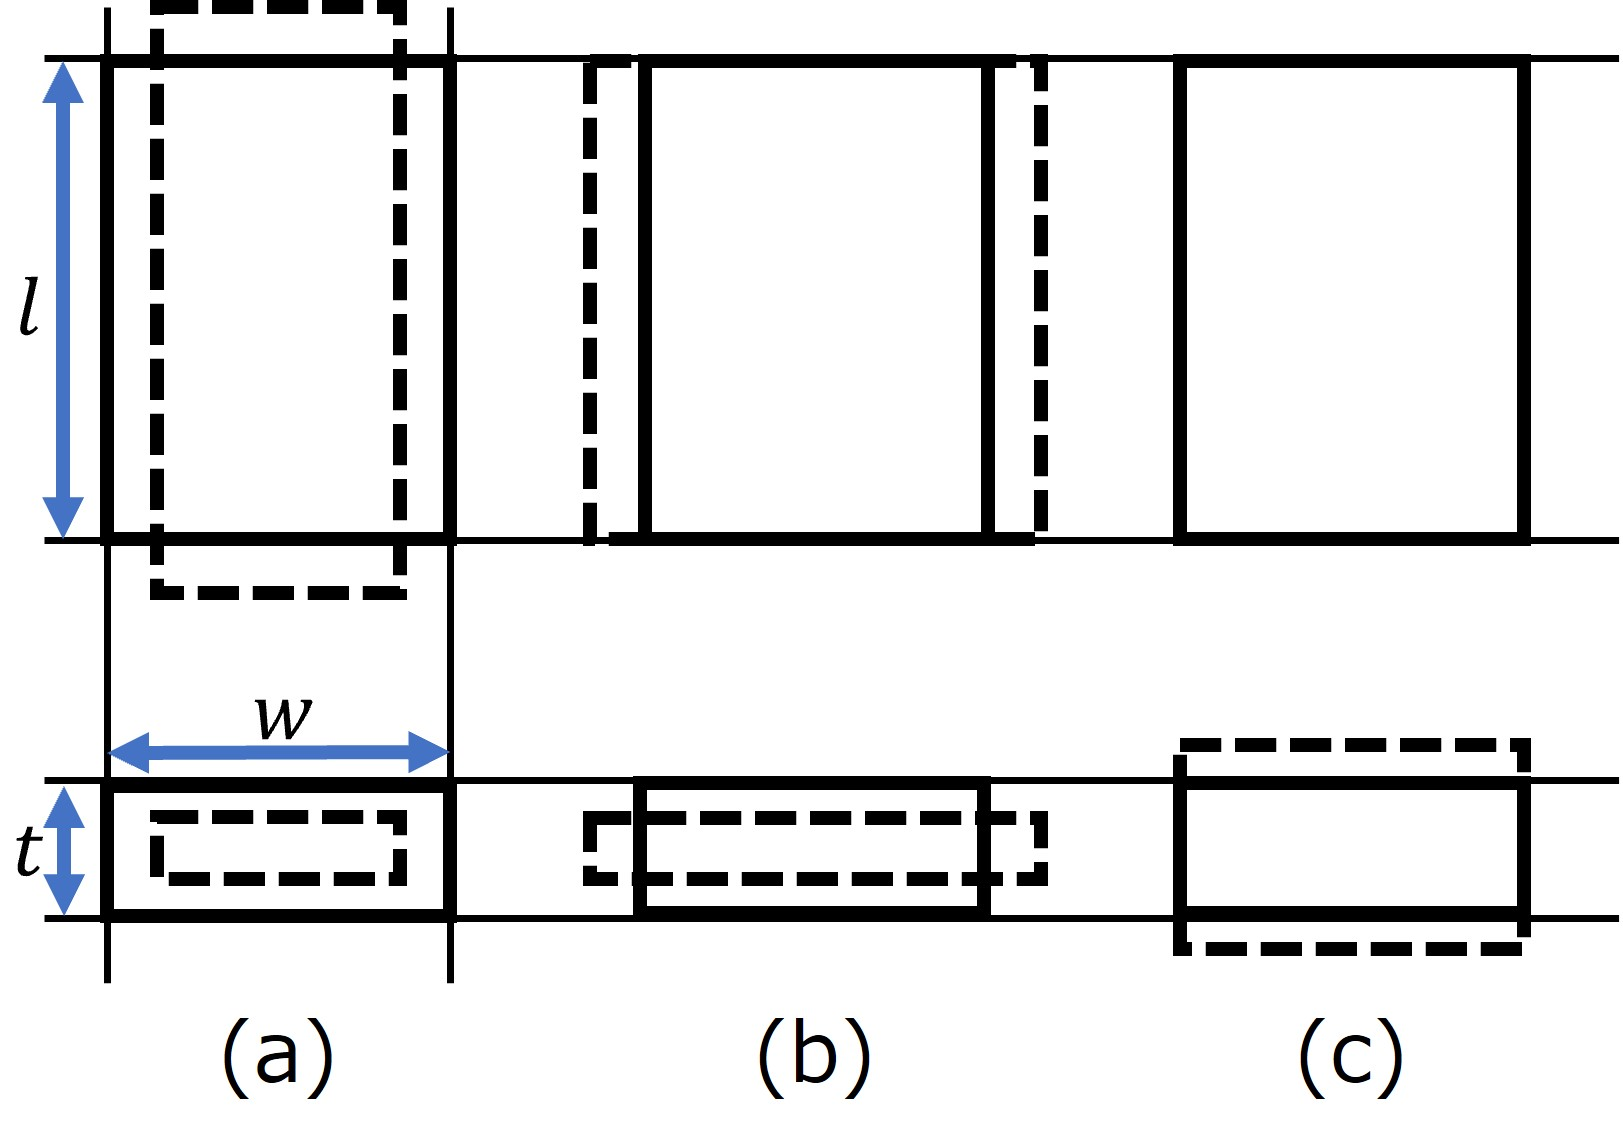
\includegraphics[width=0.6\linewidth]{圧電共鳴.jpg}
				\caption{長さ方向、幅方向、厚さ方向に圧電生を持つ材料の圧電共鳴。(a) 長さ方向の共鳴、
				(b) 幅方向の共鳴、(c) 厚さ方向の共鳴。
				$l$は試料の長さ方向の寸法、$w$は幅方向の寸法、$t$は厚さ方向の寸法。}
				\label{圧電共鳴のモード}
			\end{figure}
			\begin{figure}[h]
				\centering
				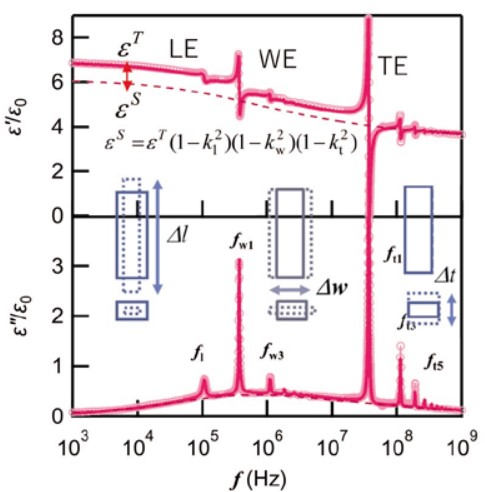
\includegraphics[width=0.5\linewidth]{VDF_TrFe_圧電共鳴.jpg}
				\caption{VDF-TrFEの圧電共鳴スペクトル\cite{小林理研ニュース}}
				\label{VDF-TrFEの圧電共鳴スペクトル}
			\end{figure}
			\\ \\
			長さ方向の共鳴が発生する周波数を$f_l$、幅方向の共鳴の周波数を$f_w$、
			厚さ方向の共鳴の周波数を$f_t$はそれぞれの寸法を$l, w, t$として
			以下の3式で表される。
			\begin{equation}
				f_l = \frac{1}{2l}\sqrt{\frac{1}{\rho s_l}}
			\end{equation} 
			\begin{equation}
				f_w = \frac{1}{2w}\sqrt{\frac{1}{\rho s_w}}
			\end{equation}
			\begin{equation}
				f_t = \frac{1}{2t}\sqrt{\frac{c_t}{\rho}}
			\end{equation} 
			また、電気機械結合係数は0°カットであれば、それぞれ方向において以下のように決まる。
			\begin{equation}
				k_l^2 = \frac{d_{31}^2}{\varepsilon_{33}^T s_{11}}
			\end{equation}
			\begin{equation}
				k_w^2 = \frac{\left(d_{32} - d_{31}s_{12}/s_{22} \right)^2}
				{\varepsilon_{33}^T s_{22}}
			\end{equation}
			\begin{equation}
				k_t^2 = \frac{e_{33}^2}{\varepsilon_{33}^S c_{33}}
			\end{equation}
			誘電率全体を上の3式を用いて以下の様に記述される。
			$\varepsilon_{33}^S$は3軸どの方向においてもひずみがない、
			あるいは固定端であるときの誘電率であり、式\eqref{Havriliak-Negami}のHavriliak-Negamiの式と同値である。
			\begin{equation}
				\varepsilon_{33} =
				\varepsilon_{33}^S
				\frac{\left(1+\frac{k_l^2}{1-k_l^2}\frac{\tan{\pi f/2f_l}}{\pi f/2f_l}\right)
				\left( 
					1+\frac{k_w^2}{1-k_w^2}\frac{\tan{\pi f/2f_w}}{\pi f/2f_w}
				\right)
				}
				{1-k_t^2\frac{\tan{\pi f/2f_t}}{\pi f/2f_t}}
				\label{normal_piezo_resonance}
			\end{equation}
			\\
			ずり圧電の共鳴モードは図\ref{圧電共鳴のモード}と異なる。
			ずり圧電の場合は、図\ref{ずり圧電の共鳴モード}(a)の様に
			配向軸に対して$\theta=45^\circ$にて正方形にカットした場合にて
			図\ref{ずり圧電の共鳴モード}(b)の共鳴モードとなる。
			正方形であるため、共鳴モードは一つしかない。
			どの試料の辺においても境界条件は自由端となる。
			また、試料の厚さは長さや幅に対して十分小さいとみなして固定端条件となる。
			この条件は、PVDFやVDF-TrFEなどにおける、厚さ方向の共鳴と同じである。
			また、ずり圧電は慣例的に膜厚方向を1軸、配向軸に垂直な方向をy軸、配向軸に平行な方向をz軸とる。
			ずり圧電の性質をもつ材料としてPLLA(ポリ乳酸)がある。
			PLLAにおける圧電スペクトルは図\ref{PLLA_piezo_resonance}の通りである。
			\begin{figure}[h]
				\centering
				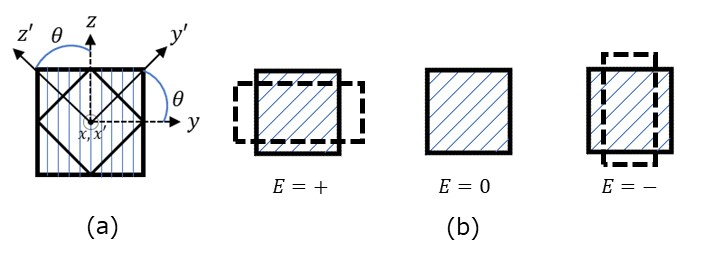
\includegraphics[width=0.8\linewidth]{ずり圧電_共鳴モード.jpg}
				\caption{ずり圧電の共鳴モード。(a) 配向軸に対して$\theta=45^\circ$の角度で正方形に切り出す。
				膜厚方向をx軸、試料平面内にy, z軸を取る。
				(b) ずり圧電のイメージ図。}
				\label{ずり圧電の共鳴モード}
			\end{figure}
			\begin{figure}[h]
				\centering
				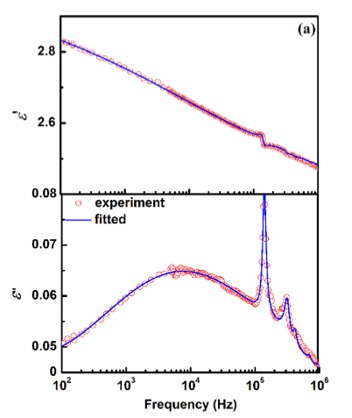
\includegraphics{PLLA_圧電共鳴スペクトル.jpg}
				\caption{ずり圧電の性質をもつPLLAの圧電共鳴スペクトル\cite{plla_piezo_resonance}}
				\label{PLLA_piezo_resonance}
			\end{figure}
			共鳴周波数$f_R$、誘電率の周波数特性$\varepsilon_{11}^T$、電気機械結合係数$k_{14}$は式\eqref{ずりの共鳴周波数}、
			式\eqref{ずりの圧電共鳴_理論式}、式\eqref{ずりの電気機械結合係数}で記述される。
			式\eqref{ずりの圧電共鳴_理論式}における$\varepsilon_{11}^S$は
			式\eqref{normal_piezo_resonance}同様に式\eqref{Havriliak-Negami}のHavriliak-Negamiの式と同値である。
			\begin{equation}
				f_R = \frac{1}{2l}\sqrt{\frac{2c_{44}}{\rho}}
				\label{ずりの共鳴周波数}
			\end{equation}
			\begin{equation}
				\varepsilon_{11}^T=\varepsilon_{11}^S\left(1+k_{14}^2\frac{\tan{\pi f/2f_R}}{\pi f/2f_R}\right)
				\label{ずりの圧電共鳴_理論式}
			\end{equation}
			\begin{equation}
				k_{14}^2=\frac{e_{14}^2}{\varepsilon_{11}^Sc_{44}}
				\label{ずりの電気機械結合係数}
			\end{equation}
			図\ref{PLA_45_cut}のように試料を正方形ではなく、
			長方形にカットして圧電共鳴スペクトルを観測した事例もある
			\cite{PLA_長方形_圧電共鳴}。
			\newpage
			\begin{figure}[h]
				\centering
				\begin{minipage}{0.45\hsize}
					\centering
					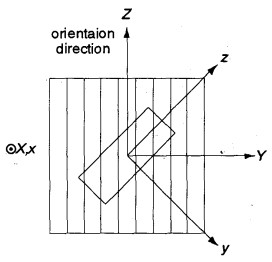
\includegraphics{PLA_ずり圧電_長方形カット.jpg}
					\caption{PLAの長方形$45^\circ$カット\cite{PLA_長方形_圧電共鳴}}
					\label{PLA_45_cut}
				\end{minipage}
				\begin{minipage}{0.45\hsize}
					\centering
					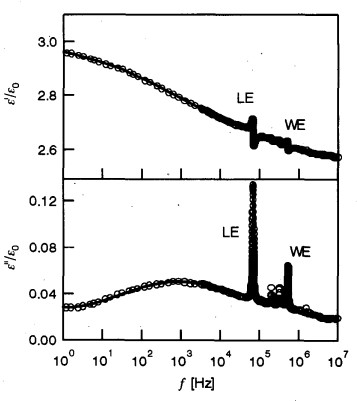
\includegraphics{PLA_圧電共鳴スペクトル_長方形.jpg}
					\caption{PLAの長方形$45^{\circ}$カットにおける圧電共鳴スペクトル観測\cite{PLA_長方形_圧電共鳴}}
				\end{minipage}
			\end{figure}
			\newpage
			\section{逆平行$\beta$ シート構造におけるずりの圧電性}
			$\alpha$ヘリックス構造の分子を持ち、大きな圧電性が期待できるPLLAは理論、実験、
			デバイス応用まで進んでいる。しかし、蛋白質の二次構造として$\alpha$ヘリックス以外にも
			$\beta$ シート構造も取りうる。本研究の材料であるシルクは逆平行$\beta$シートを構成する。
			デバイス応用などの社会実装は進んでいないが$\beta$シート構造も
			圧電性が生じると報告されている\cite{beta_sheet_piezo_theory}。
			
			逆平行$\beta$ シートの構造は図\ref{逆平行ベータシート}の通りである。
			図\ref{逆平行ベータシート}(A)の通り、分子間で水素結合した構造である。
			水素結合により、酸素原子Oにおいて窒素原子Nに向って引っ張る力$f$が図\ref{逆平行ベータシート}(B)の通り
			存在する。平衡状態においては図\ref{逆平行ベータシート_力}において酸素原子Oから窒素原子Nの方向である
			ADを向いている。ずりの力が加えられたときに酸素原子が図\ref{逆平行ベータシート}の分子鎖方向、
			図\ref{逆平行ベータシート_力}におけるAE方向に移動する現象は現実的ではない。
			よってずりの力が加えられたときに酸素原子Oは図\ref{逆平行ベータシート_力}におけるAB方向に移動する。
			よって図\ref{逆平行ベータシート}、図\ref{逆平行ベータシート_力}における$f$は三次元的に向きを変え、
			逆平行$\beta$シートの表裏方向に電荷の偏りが生じる。
			単純なモデルでは逆平行$\beta$シートの圧電性はこのようにして理解されている。

			\begin{figure}[h]
				\centering
				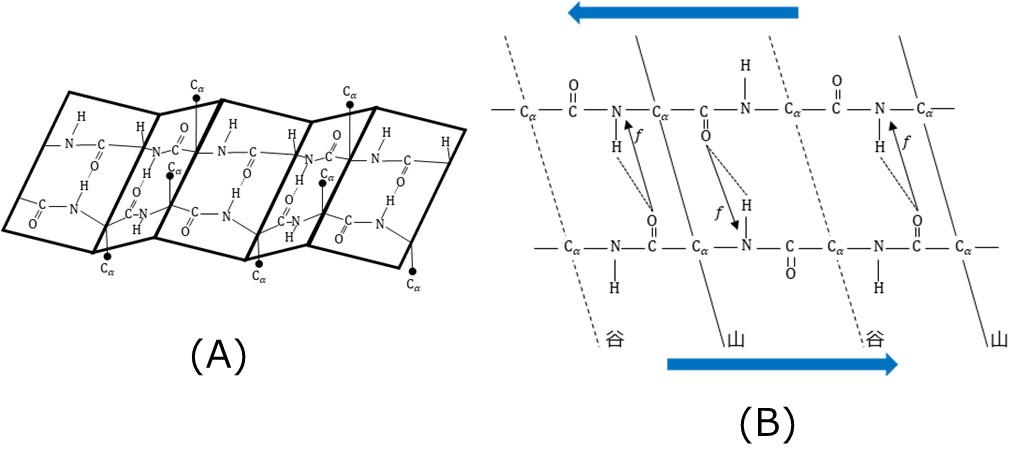
\includegraphics[width=0.9\linewidth]{anti_parallel_beta.jpg}
				\caption{1枚の逆平行$\beta$シートの構造。(A)三次元における逆平行$\beta$シート、
				(B)上からみた逆平行$\beta$シート。青の矢印はずりの力を加える方向。}
				\label{逆平行ベータシート}
			\end{figure}
			\begin{figure}[H]
				\centering
				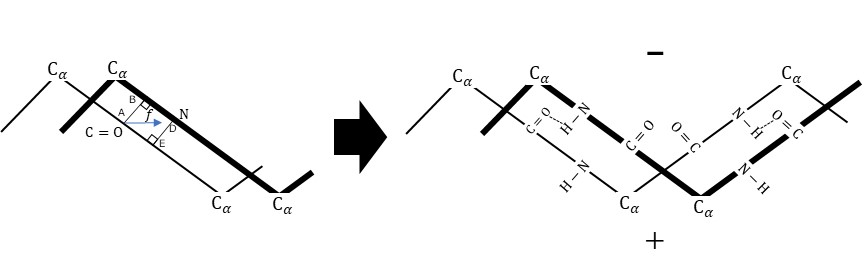
\includegraphics[width=0.9\linewidth]{anit_parallel_force.jpg}
				\caption{1枚の逆平行$\beta$シートの構造でずりの力が加えられたときの横からみた変動。
				矢印前が平衡状態、矢印後がずりの力が加えられている状態。}
				\label{逆平行ベータシート_力}
			\end{figure}
			\newpage
			\section{$\alpha$ ヘリックス構造におけるずりの圧電性}
			螺旋構造を持ち、ずりの圧電性を有する物質として
			PLLAがある。
			蛋白質の$\alpha$ヘリックスとは異なるが、
			PLLAにおけるずりの圧電性を簡単なモデルにて説明し、
			それを拡張すると$\alpha$ ヘリックスにおけるずりの圧電性の
			簡易的な説明となる。
			PLLAは図\ref{alpha_helix_1}(A)の様な螺旋分子をとる。
			この際に、螺旋分子の中心軸方向を3軸に取る。
			螺旋分子は応力を印加する平面において1軸方向に対し
			図\ref{alpha_helix_1}(B)の通り、正の領域と負の領域が存在する。
			簡易的に4つ線分で一周する4/1螺旋構造を想定し、
			それに対応する4領域が図\ref{alpha_helix_1}(C)である。
			PLLAはC=O結合において双極子を有する。そのO原子は常に螺旋分子の
			中心軸側を向いている。分子内の水素結合を考慮しない。
			図\ref{alpha_helix_2}に対応する。
			ずり応力を印加すると山領域においては伸び、谷領域では縮む。
			\begin{figure}[h]
				\centering
				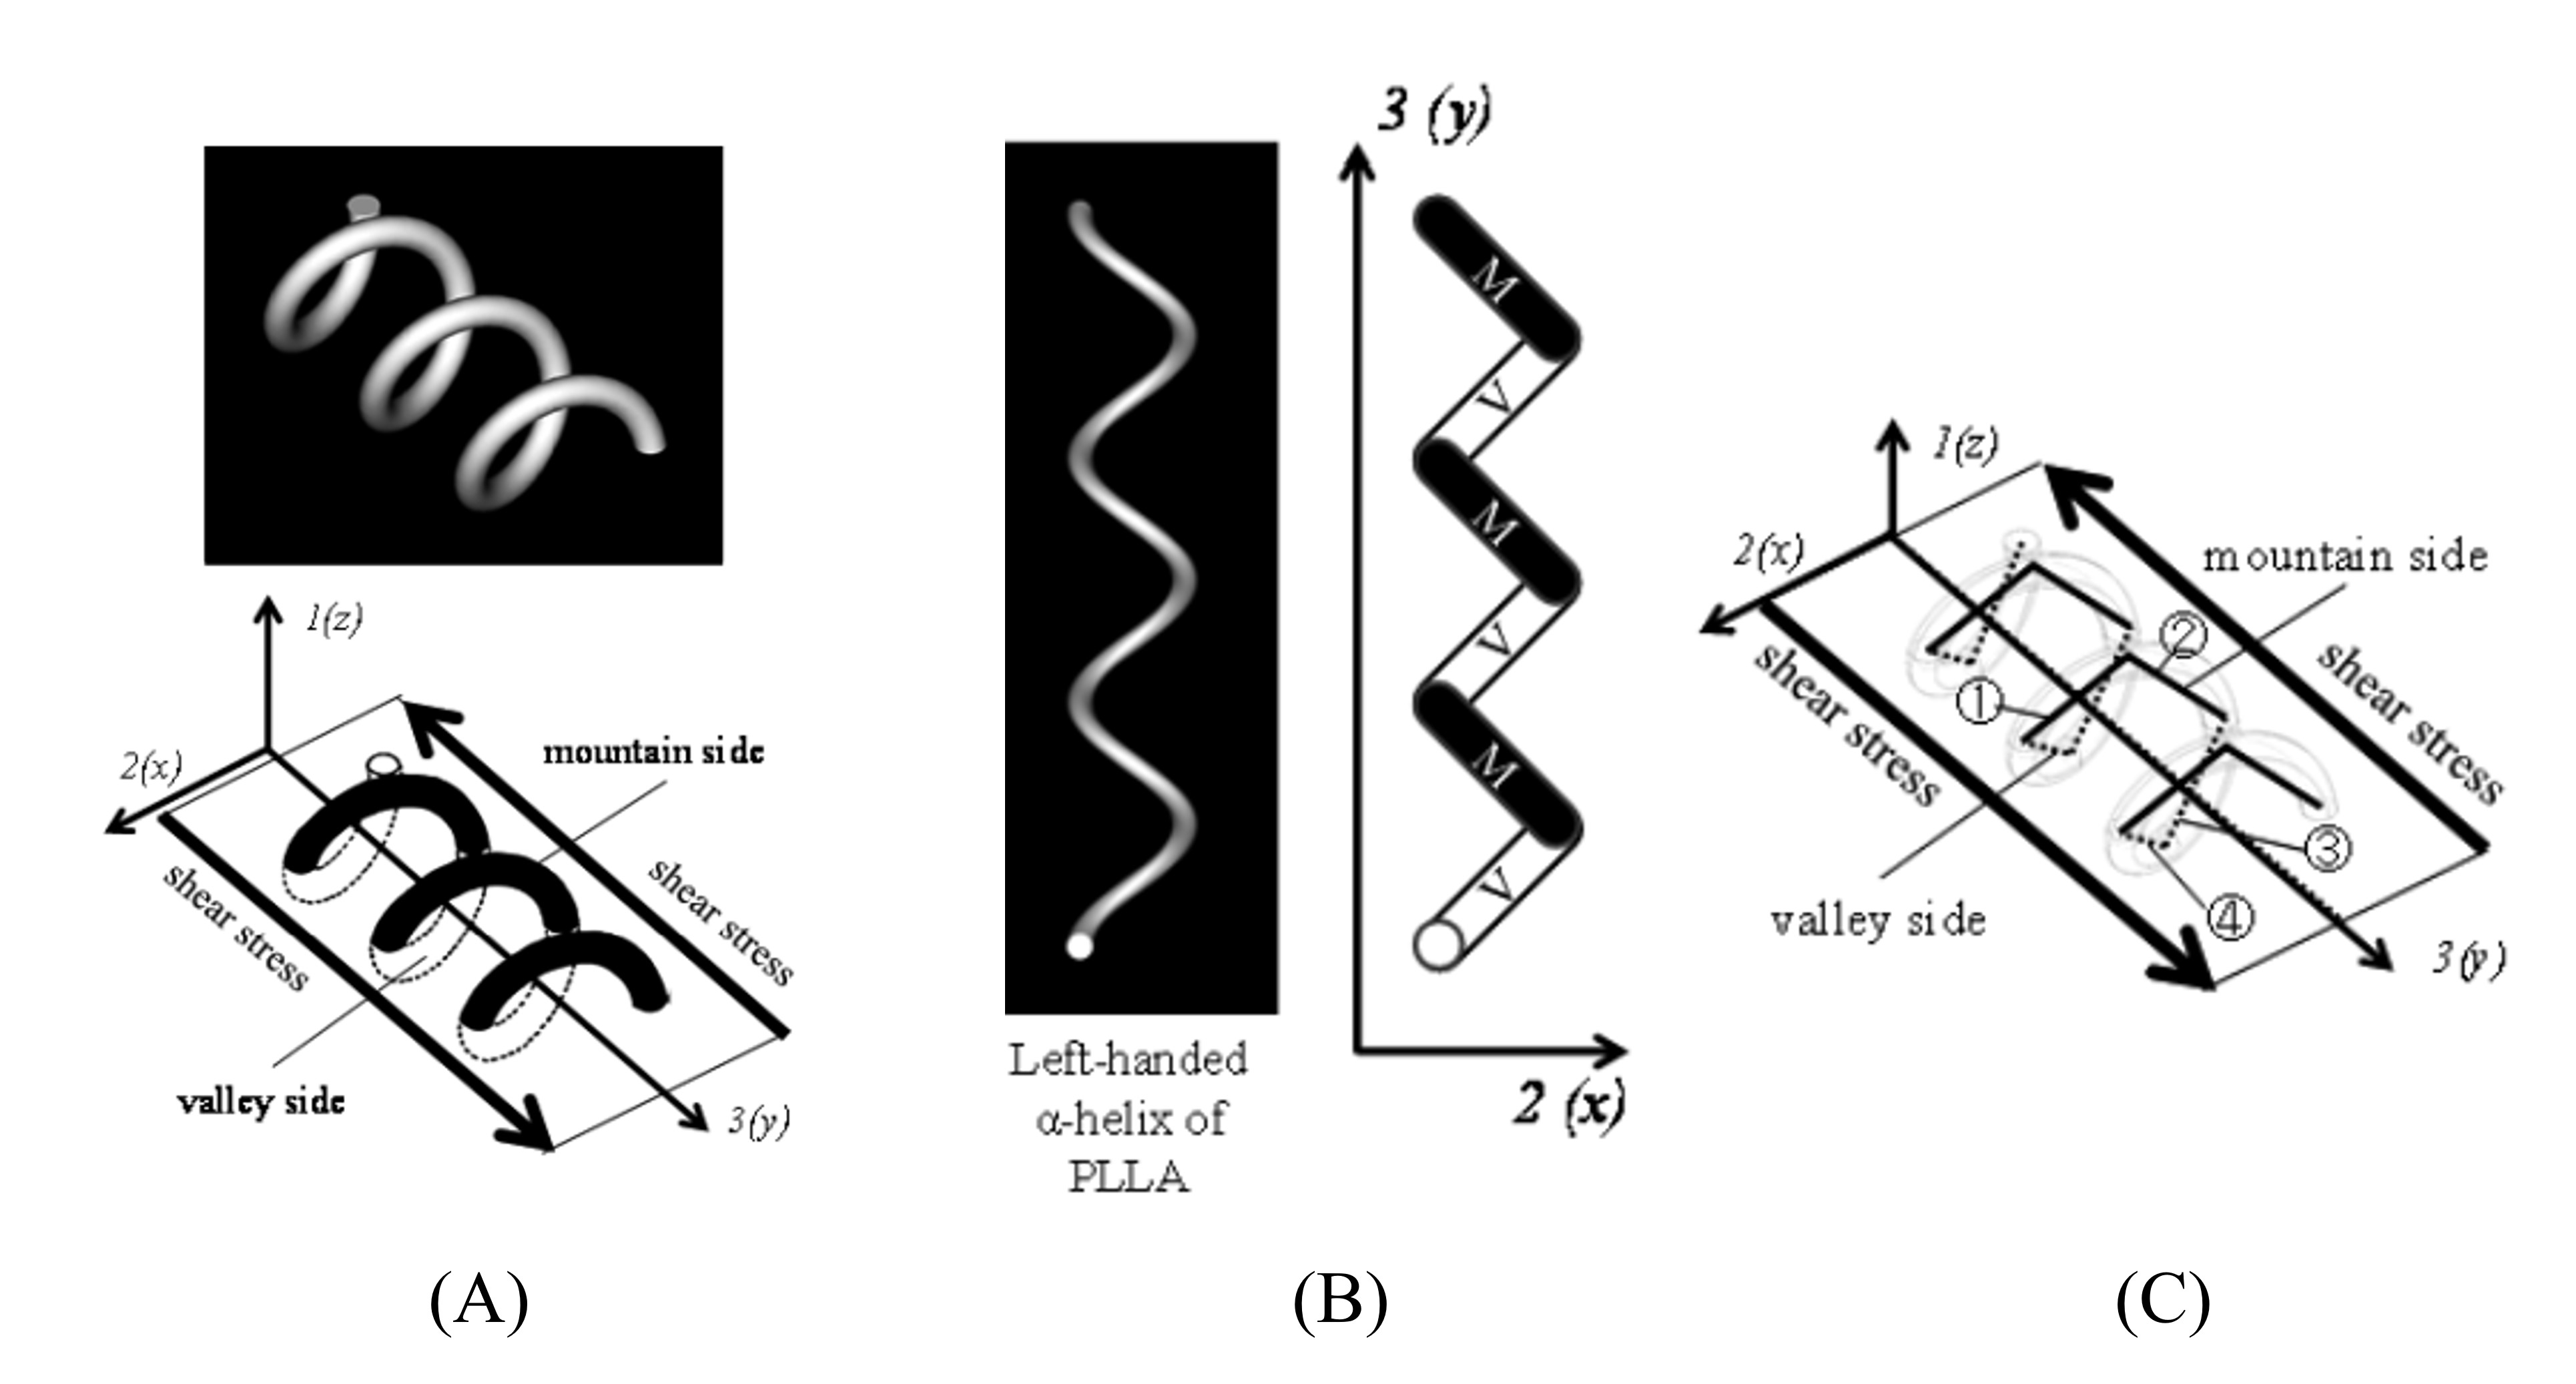
\includegraphics[width=0.9\linewidth]{alpha_helix_piezo.jpg}
				\caption{PLLAの螺旋分子とずり応力\cite{吉田光伸2016ポリ乳酸を用いた固相延伸フィルムの高圧電性発現機構の検討}。
				(A)PLLAの螺旋分子とずり応力の関係と座標軸、
				(B)螺旋分子に加えられるずり応力平面に対する山と谷の領域、
				(C)螺旋分子1周における山と谷の4領域。}
				\label{alpha_helix_1}
			\end{figure}
			\begin{figure}[H]
				\centering
				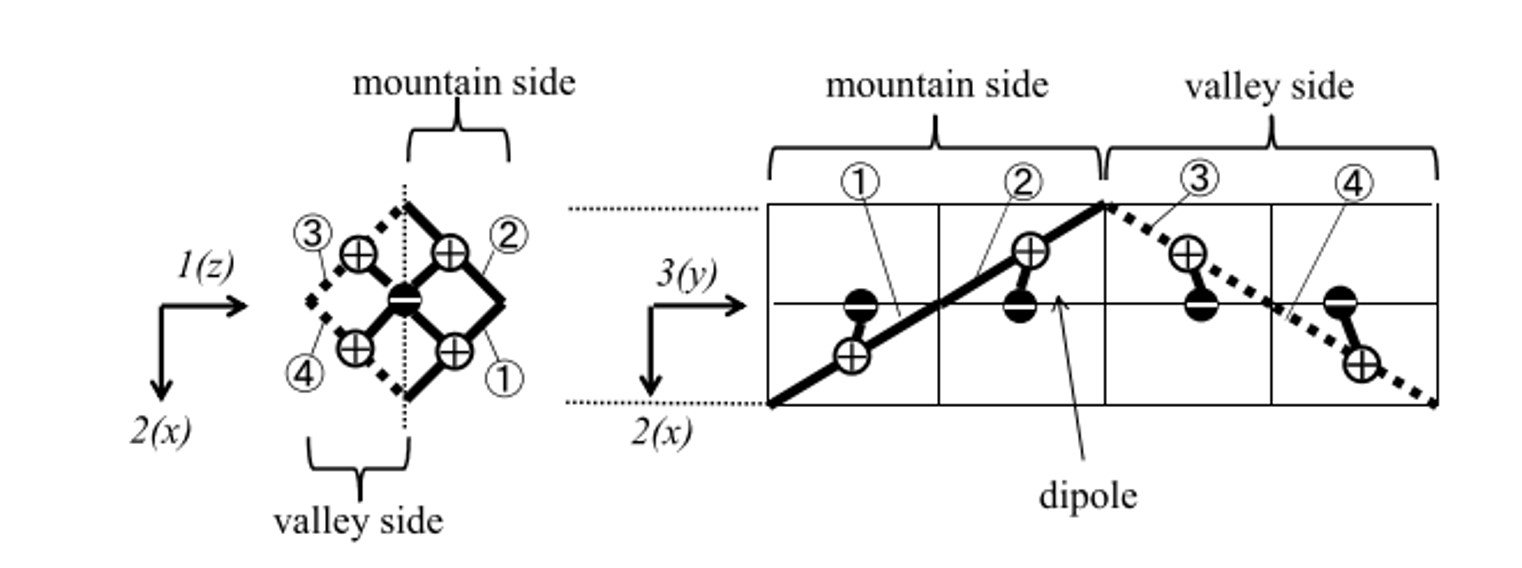
\includegraphics[width=0.8\linewidth]{PLLA_4領域_dipole.jpg}
				\caption{4/1螺旋モデルと双極子(C=O)の関係\cite{吉田光伸2016ポリ乳酸を用いた固相延伸フィルムの高圧電性発現機構の検討}。
				}
				\label{alpha_helix_2}
			\end{figure}
			\newpage
			ずり応力が印加されると縮む、山領域においては図\ref{alpha_helix_3}(A)
			の通り双極子の回転を生じる。図\ref{alpha_helix_3}(B)の通り、
			変形後は分極を生じる。
			また、ずり応力が印加されると伸びる谷領域では
			図\ref{alpha_helix_4}(A)
			の通り双極子の回転を生じる。図\ref{alpha_helix_4}(B)の通り、
			変形後は分極を生じる。
			山領域、谷領域どちらも変形後の分極の揃っているため、大きな圧電性を生じる。
			蛋白質の$\alpha$ ヘリックスは分子内で水素結合しており、C=O結合が
			螺旋中心軸に向いておらず、平行となる。
			しかし、ずり応力に生じる双極子の回転角度が減少するだけで、PLLAのモデルを拡張するだけとなる。
			\begin{figure}[h]
				\centering
				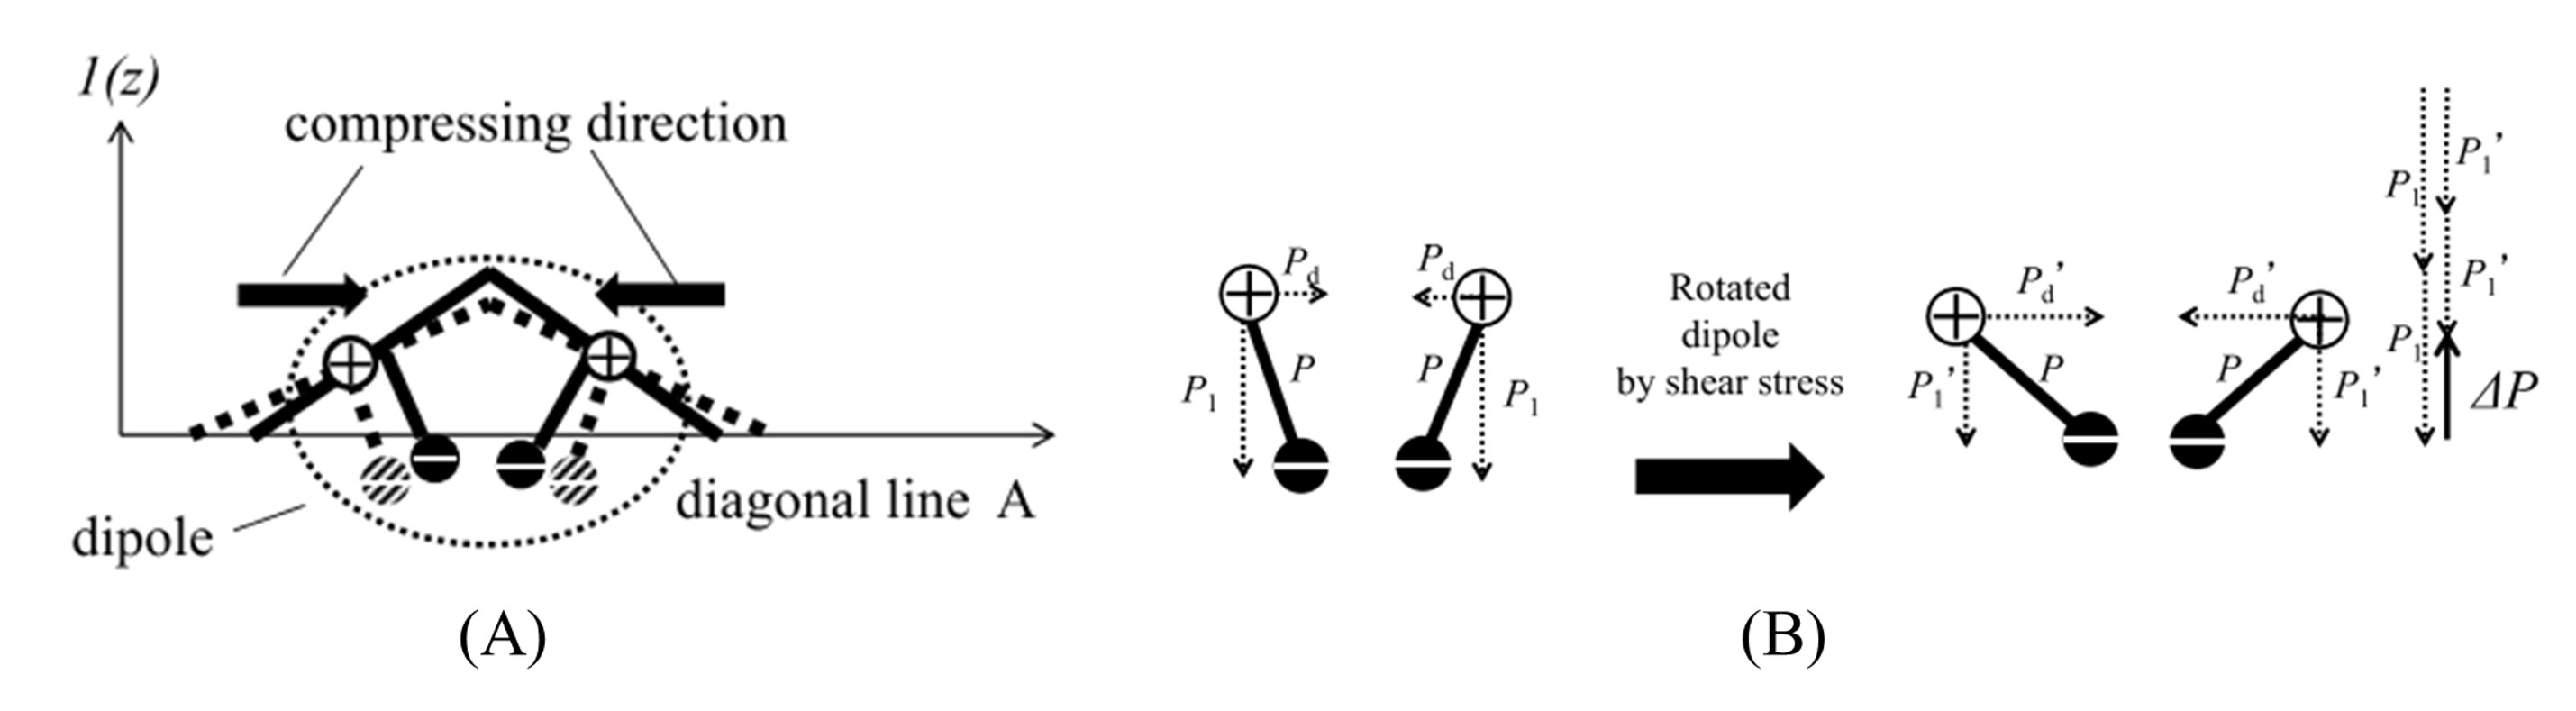
\includegraphics[width=\linewidth]{plla_yama.jpg}
				\caption{4/1螺旋分子モデルの山領域におけるずり応力の変形\cite{吉田光伸2016ポリ乳酸を用いた固相延伸フィルムの高圧電性発現機構の検討}。
				(A)双極子の回転、
				(B)双極子の回転と分極$\Delta P$。
				}
				\label{alpha_helix_3}
			\end{figure}
			\begin{figure}[h]
				\centering
				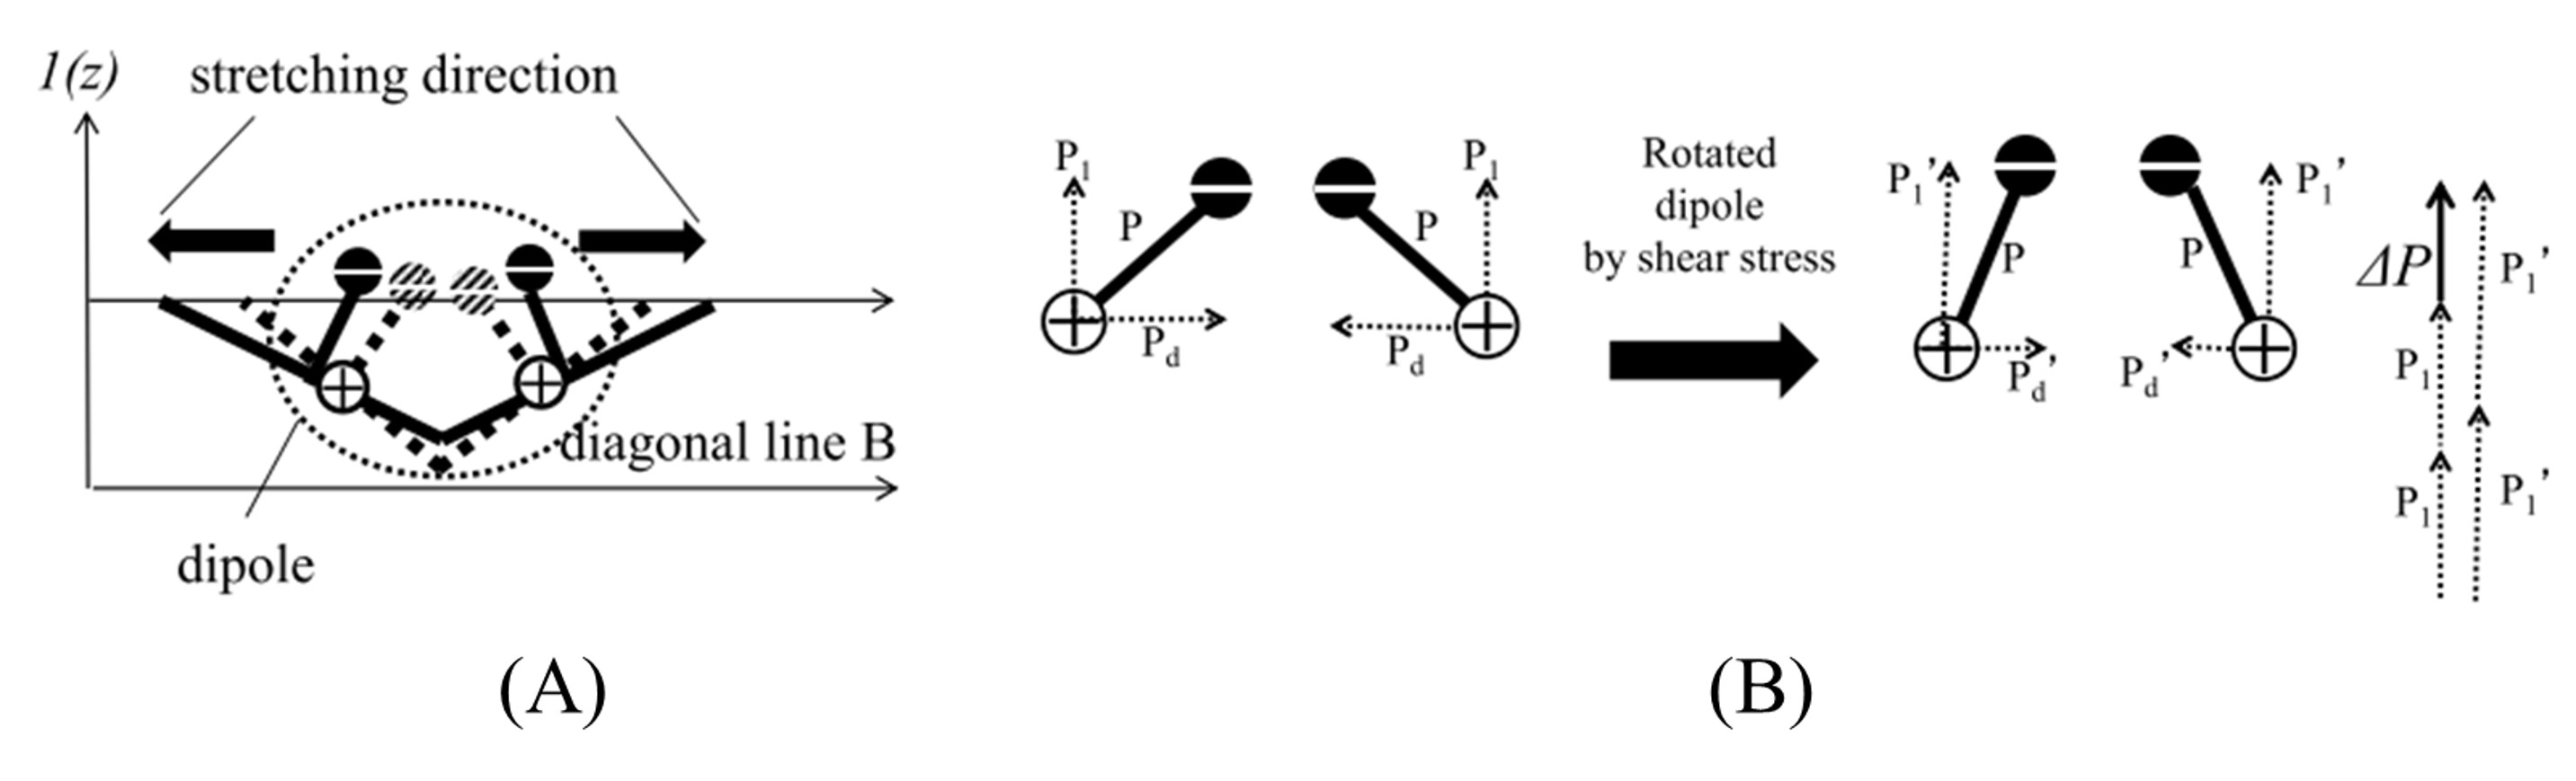
\includegraphics[width=\linewidth]{plla_tani.jpg}
				\caption{4/1螺旋分子モデルの谷領域におけるずり応力の変形\cite{吉田光伸2016ポリ乳酸を用いた固相延伸フィルムの高圧電性発現機構の検討}。
				(A)双極子の回転、
				(B)双極子の回転と分極$\Delta P$。
				}
				\label{alpha_helix_4}
			\end{figure}
			\newpage
	\chapter{実験手法}
		\section{熱プレスを用いたシルクフィルムの作製方法}
		本研究では
		図\ref{セリシンを含まない試料作製手順}、図\ref{セリシンを含むフィルム作製手順}
		の通り熱プレスしてシルクフィルムを作製した。
		セリシンを除去したフィルムを作製する場合は、まず、糊を用いて割りばし格子状に組み、固定し
		シルクを巻く。
		次に加熱した炭酸ナトリウム水溶液に入れ数時間放置して取り出す。
		乾燥させ割りばしにカッターで切り込みを入れシルクを外す。
		鉄板の上に並べ、若干水で濡らして2時間プレスする。
		一旦乾燥させる理由は、糸が濡れていると綺麗に並べずらいからである。
		セリシンが含まれているフィルムを作製する場合は鉄板に糸を巻いて、水で濡らし、
		上下に鉄板をさらに挟んだ状態で2時間プレスする。
		一回、熱プレスを行ってもプレスが不十分である場合がある。
		特に、セリシンを含むフィルムにおいては、糸を巻いている鉄板
		は熱プレスが不十分で、表裏で弾性の違いを生じる。
		その差が激しいとフィルムが丸まってしまう。
		そういった場合は、再び水に濡らし1枚の状態で熱プレスする。

		図\ref{試料外観}が作製したフィルムの外観である。
		セリシンなしのフィルムにおいてはフィブロイン単体で生じるとされる
		光沢が見られる。

		電極はスパッタを用いて作製した。
		その際に図\ref{金属マスク}の金属マスクを用いて角度依存性、試料寸法依存性の試料を作製した。

		\begin{figure}[h]
			\centering
			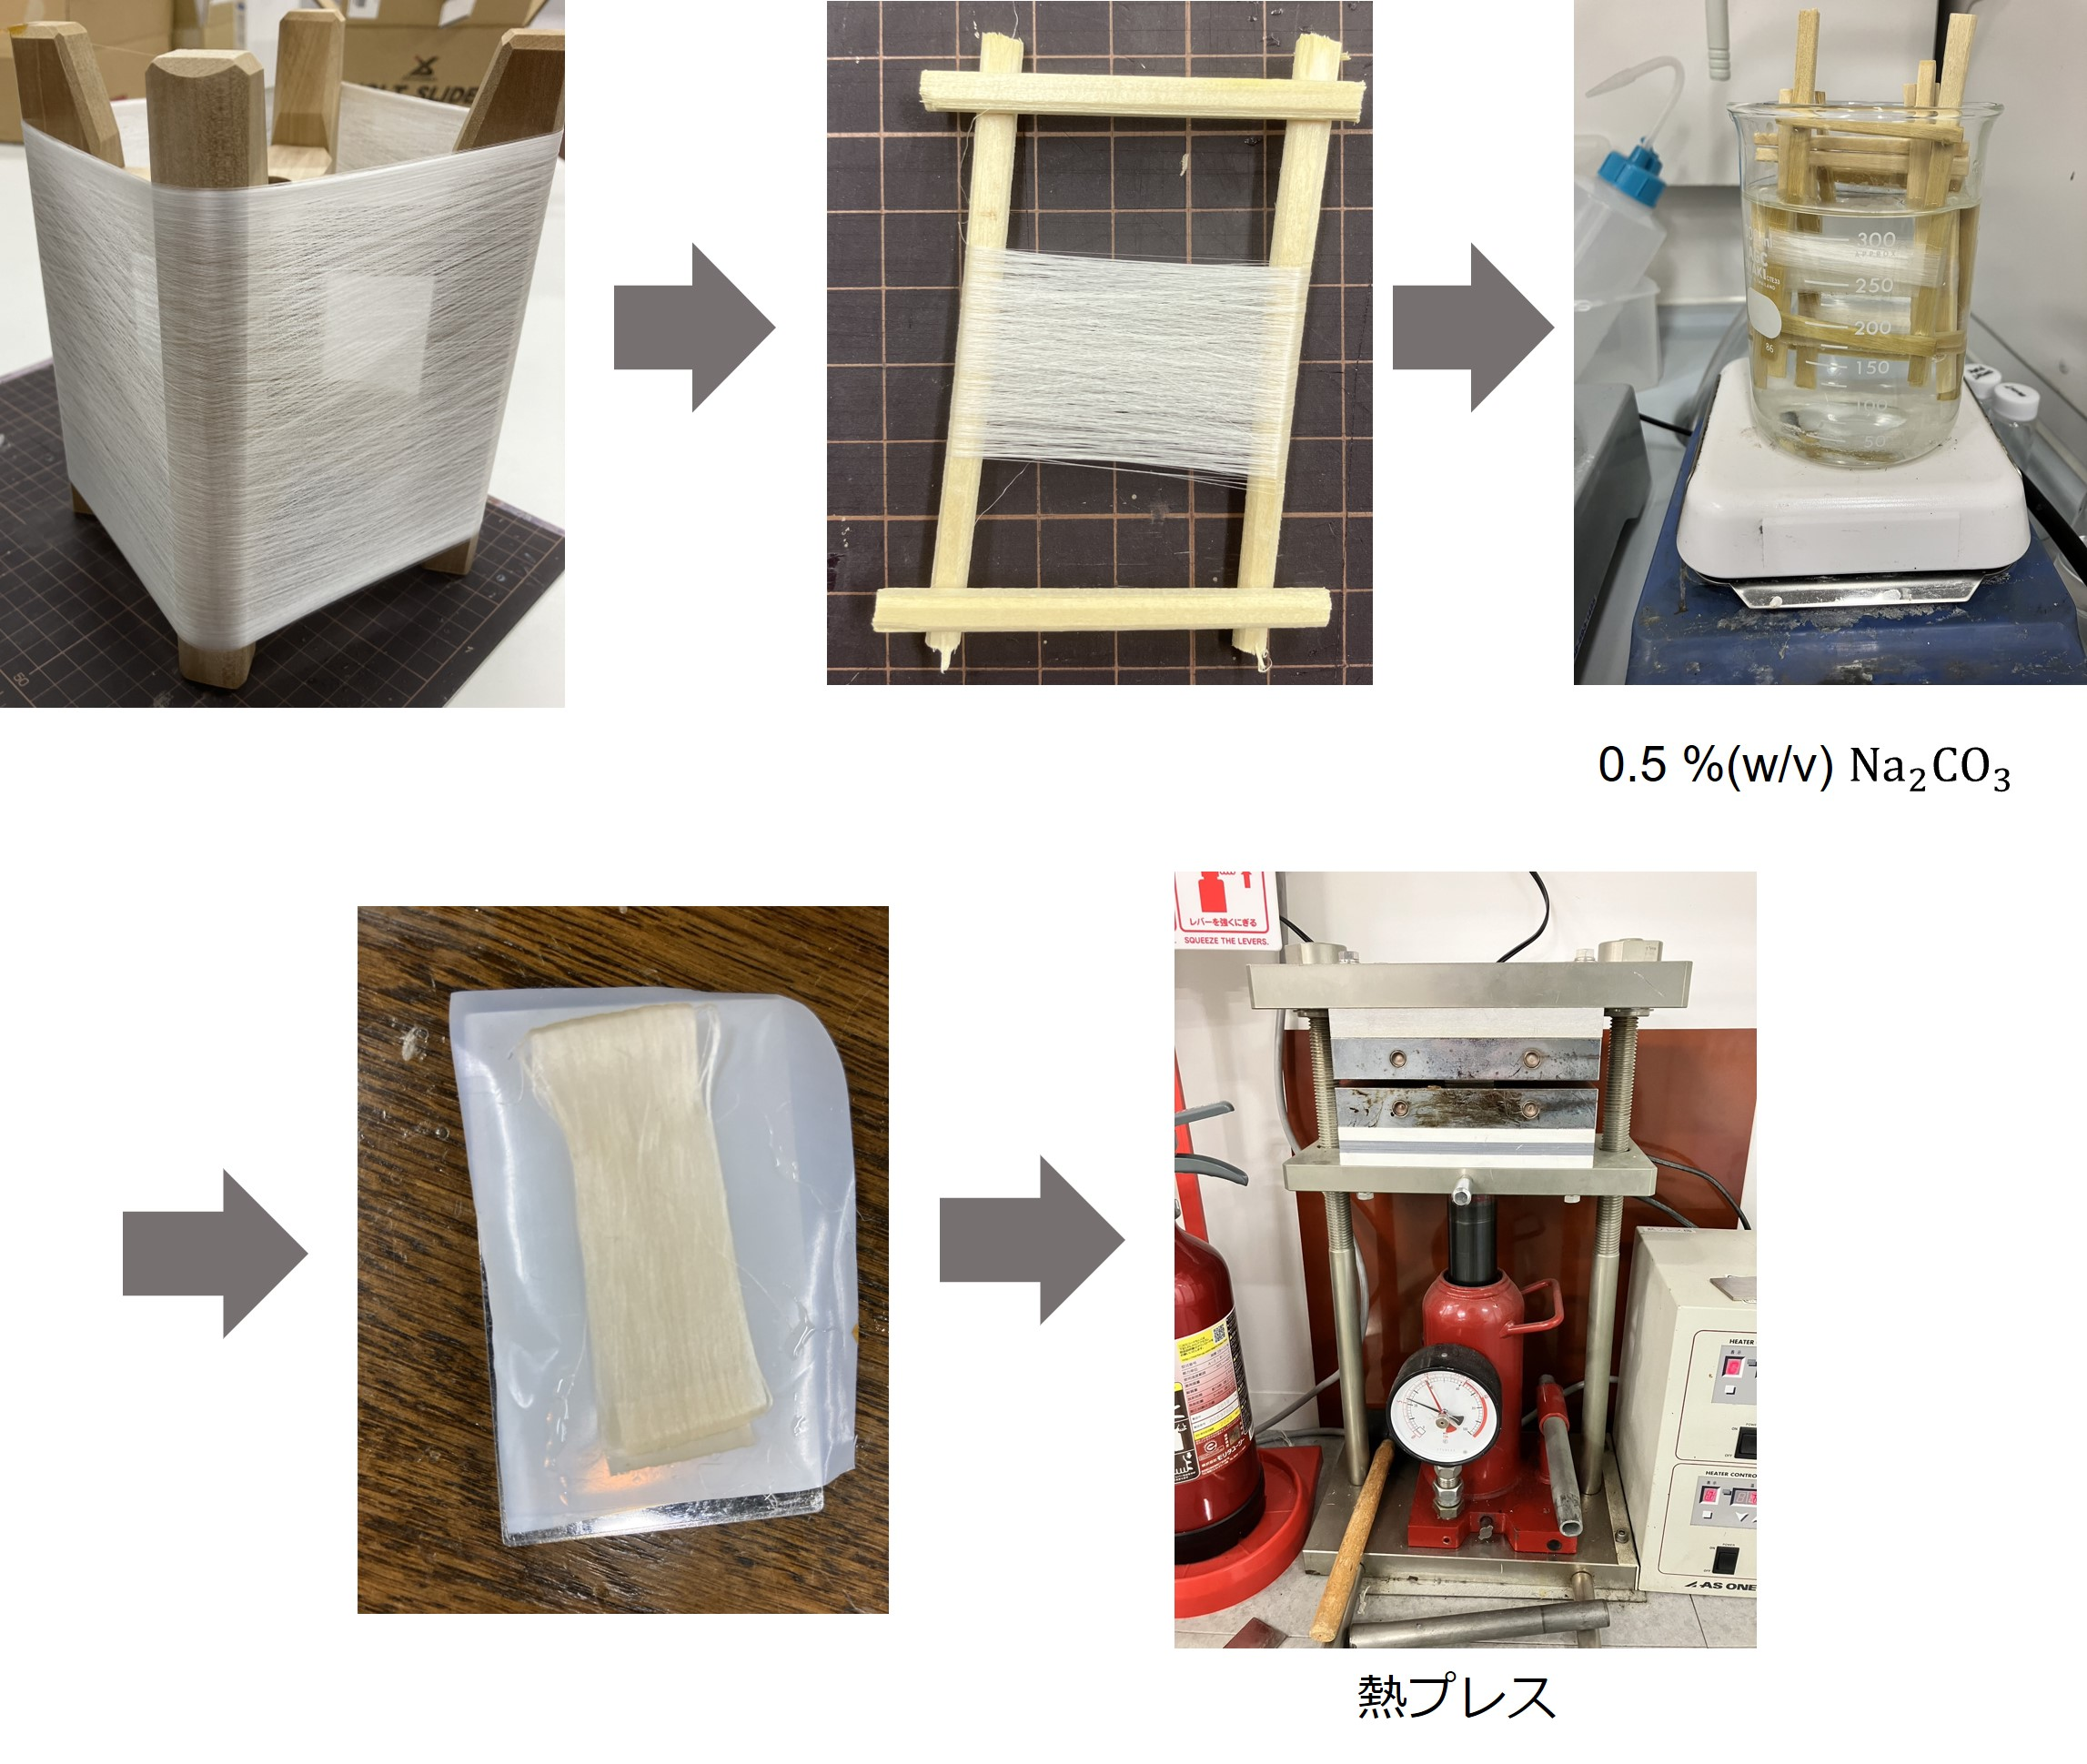
\includegraphics[scale=0.65]{試料作製手順.jpg}
			\caption{セリシンを含まないシルクフィルムの作製手順}
			\label{セリシンを含まない試料作製手順}
		\end{figure}
		\newpage
		\begin{figure}[h]
			\centering
			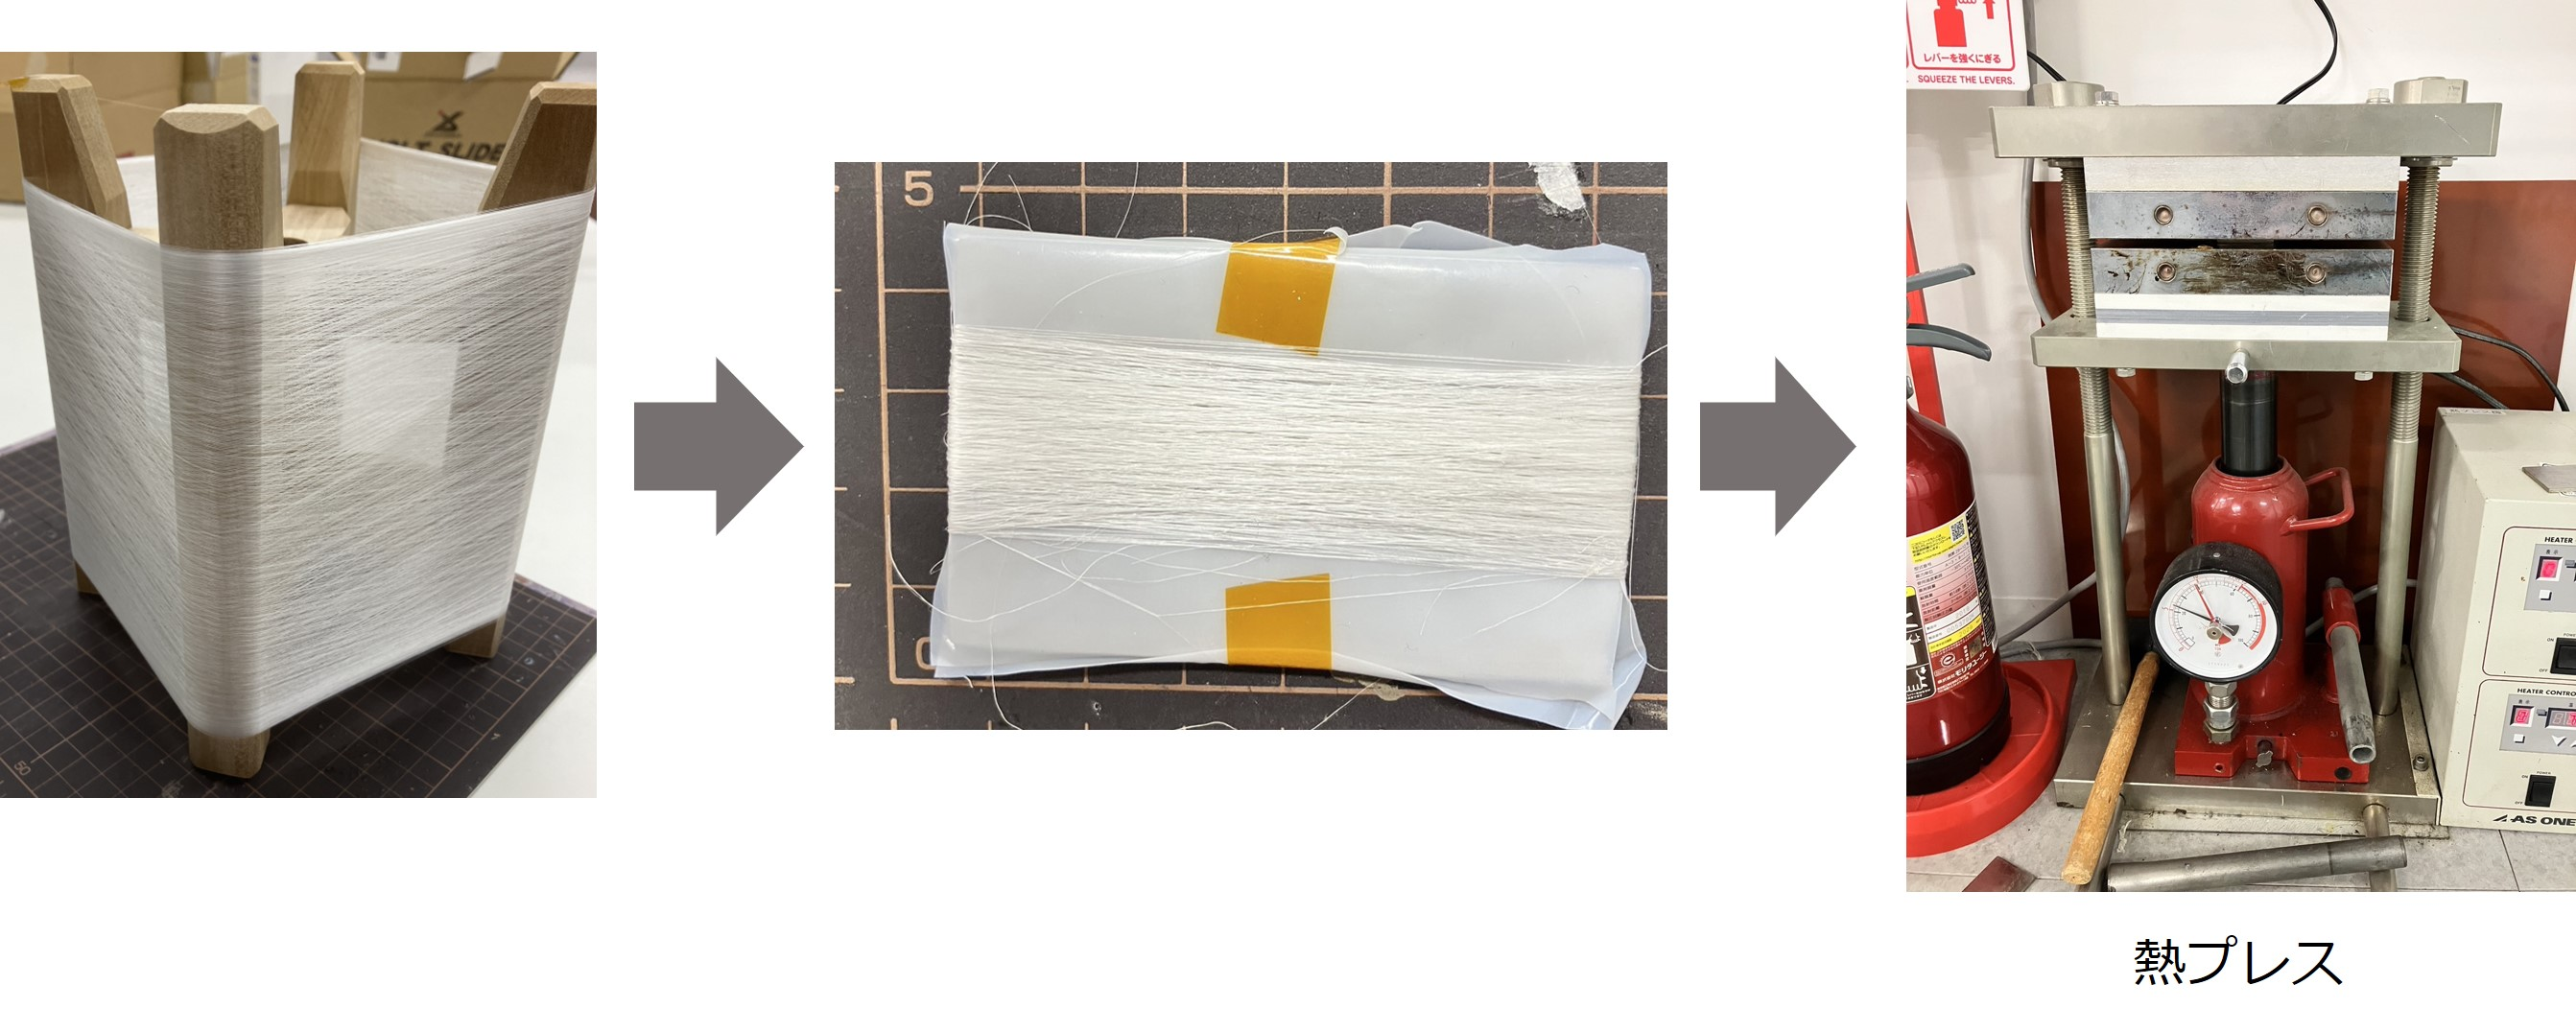
\includegraphics[width=\linewidth]{試料作製手順2.jpg}
			\caption{セリシンを含むシルクフィルムの作製手順}
			\label{セリシンを含むフィルム作製手順}
		\end{figure}
		\begin{figure}[h]
			\centering
			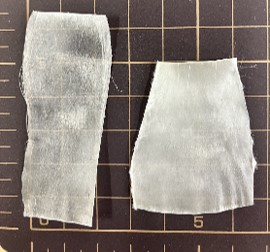
\includegraphics[scale=1]{試料.jpg}
			\caption{作製したシルクフィルム。左がセリシンを含む。右がセリシンを含まない。}
			\label{試料外観}
		\end{figure}
		\begin{figure}[H]
			\centering
			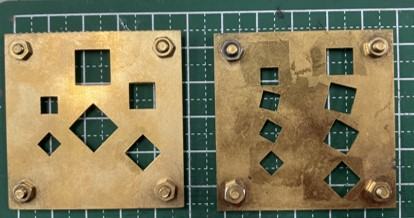
\includegraphics[scale=0.9]{金属マスク.jpg}
			\caption{作製した金属マスク}
			\label{金属マスク}
		\end{figure}

		\newpage
		\section{キャストによるシルクフィルムの作製方法}
		\label{キャストフィルムの作製方法}
		シルクからセリシンを除去したキャストフィルム作製方法は
		図\ref{フィブロインキャストフィルムの作製方法}の通りである。
		熱湯にした炭酸ナトリウム水溶液(Na$_2$CO$_3$)にシルクを入れてセリシンを除去する。
		セリシン以外のゴミも同時に除去されるためこれを繰り返す。
		その次に、塩化カルシウムCaCl$_2$と蒸留水と無水エタノール
		にシルクを混ぜて加熱すると溶解する。
		その後、透析して塩を取り除く。
		透析する前にゴミを除去するため、濾過してもよいが溶解
		直後のフィブロイン溶液は粘性が高く濾過されない場合がある。
		透析には毎日、水を入れ替えて最低3日ほど繰り返す。
		入れ替える回数、透析する時間を伸ばす程、塩が除去されると期待出来る。
		50℃以下でキャストするとSilk I型となり、50℃以上でキャストするとSilk II型となる。

		セリシンを除去していないフィルムを作製する場合は図\ref{フィブロインキャストフィルムの作製方法}の右側の
		溶解過程のみ行えばよい。
		\begin{figure}[h]
			\centering
			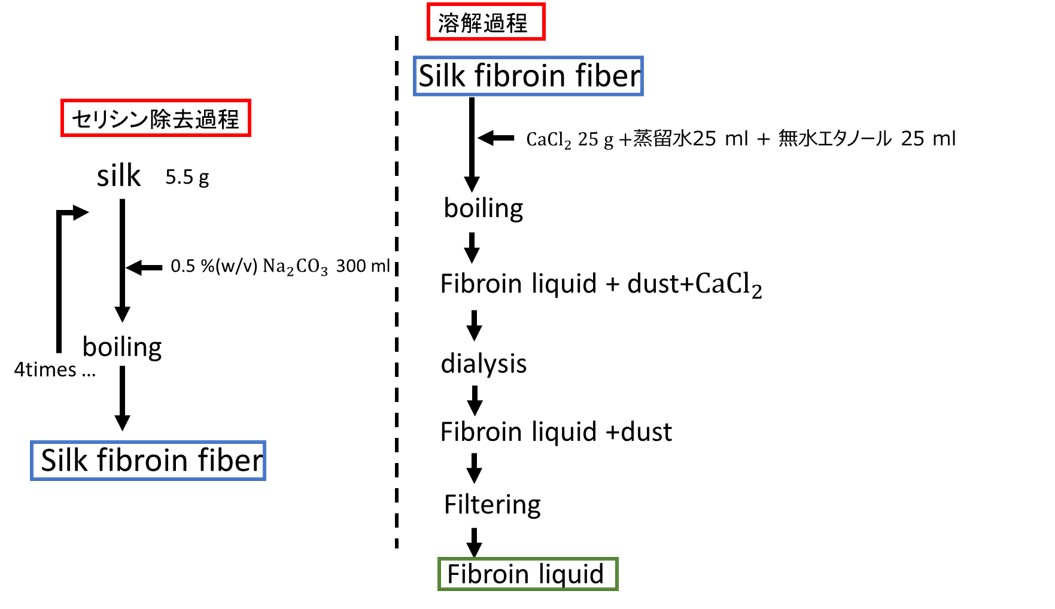
\includegraphics[scale=0.75]{cast_film_作成方法.jpg}
			\caption{キャストフィルムの作製方法\cite{フィブロイン溶解方法}.}
			\label{フィブロインキャストフィルムの作製方法}
		\end{figure}
		\\
		キャストにて作製した試料は以下の通りである。
		セリシンを除去した場合は透明になると判明した。
		\begin{figure}[H]
			\centering
			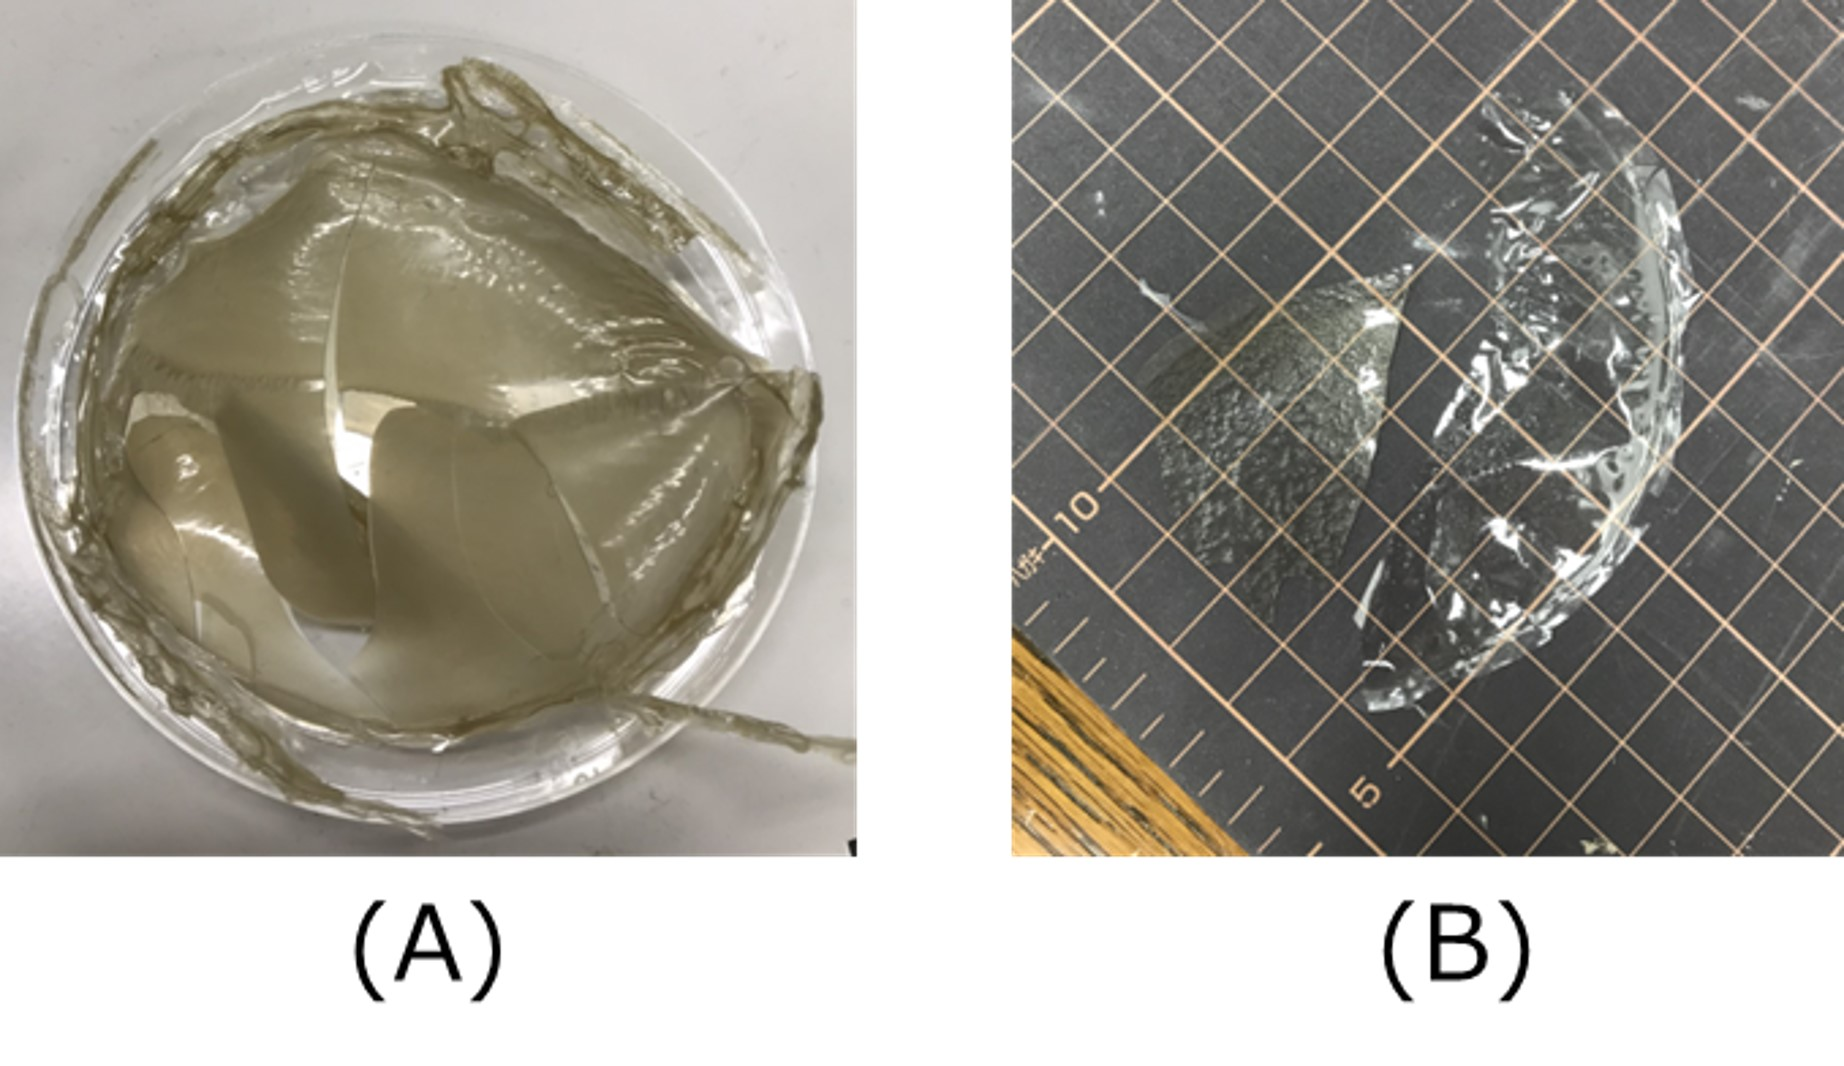
\includegraphics[scale=0.3]{cast_film_sample.jpg}
			\caption{キャストで作製した試料. (A)セリシンを除去しなった試料, (B)セリシンを除去した試料.}
		\end{figure}
		\newpage
		\section{評価方法}
			\subsection{X線回折($\theta - 2\theta$測定とPole figure測定)}
			本研究では$\theta-2\theta$測定にて
			結晶性を評価し、配向性の評価にはPole figure測定を用いた。
			\subsubsection{$\theta - 2\theta$測定}
			試料の結晶構造の解析のためにXRD(X-Ray Diffraction)の$\theta-2\theta$測定を行った。
			測定には図\ref{XRD_nakajima}に示したRINT-2000(Rigaku Corporation)を使用した。
			ある結晶粒における面間隔$d$の格子面(hkl)が入射X線に対し、式\eqref{Bragg}の式を満たすとき回折が生じる。
			\begin{equation}
				2d \sin \theta = n \lambda \ \ \ \ \ \ (n\in \mathbb{Z})
				\label{Bragg}
			\end{equation}
			このとき、回折線の方向は入射X線の方向に対して図\ref{XRD_theta_2theta}の関係がある。
			よって測定時には図\ref{集中法光学系}のようにX線源とX線検出器を走査させる。
			図\ref{XRD_theta_2theta}の赤い矢印は回折に寄与している格子面の法線方向を示している。
			格子面の法線方向、もしくは逆格子ベクトル$g_{hkl}$は測定時において入射角$\theta$を走査させても変動しない。
			よって$\theta-2\theta$測定は測定対象の全ての結晶の格子面の法線方向が測定試料の法線方向に存在している状態が望ましい。
			また、この状態を多結晶という。結晶が配向している、あるいは単結晶の場合において$\theta-2\theta$測定を行うと
			ピークが小さくなる、見れないといった現象を生じる。よって本研究では$\theta-2\theta$測定にて
			結晶性を評価し、配向性の評価にはPole figure測定を用いた。
			\begin{figure}[h]
				\centering
				\begin{minipage}{0.45\hsize}
					\centering
					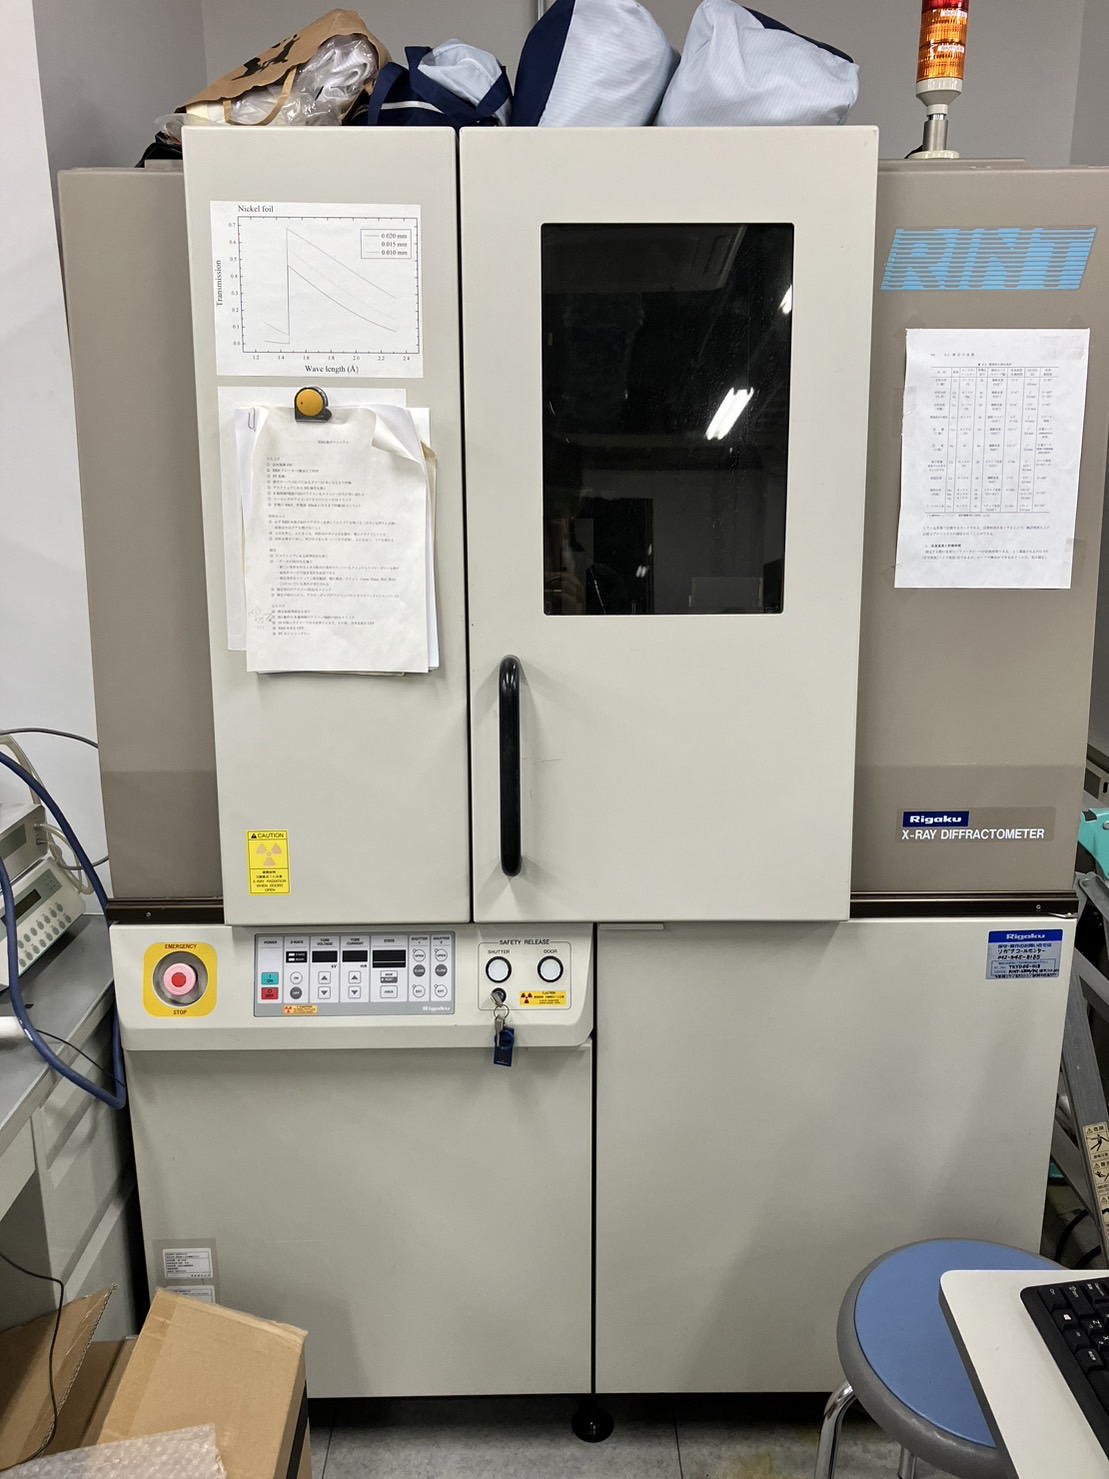
\includegraphics[width=0.9\linewidth]{rint_2000.jpg}
					\caption{RINT-2000(Rigaku Corporation)}
					\label{XRD_nakajima}
				\end{minipage}
				\begin{minipage}{0.45\hsize}
					\centering
					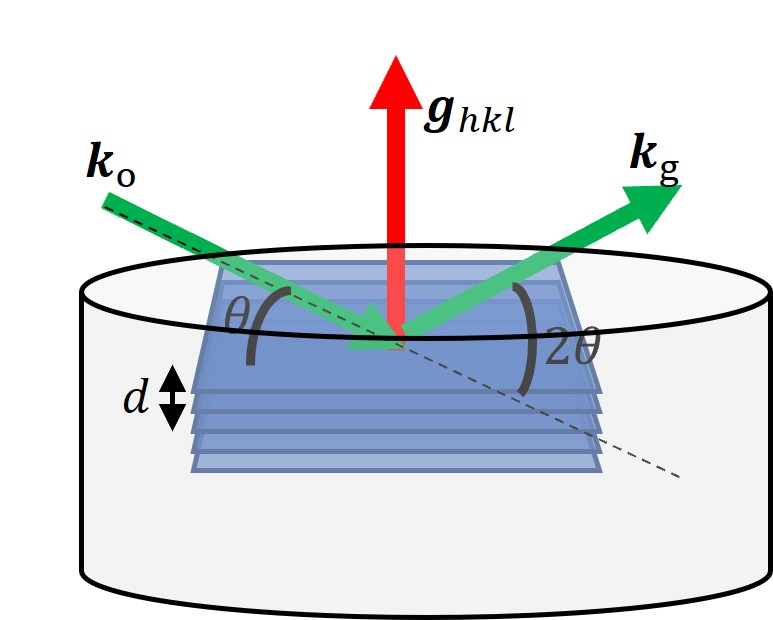
\includegraphics[scale=0.9]{theta_2theta.jpg}
					\caption{$\theta-2\theta$測定における面間隔$d$と$\theta$の関係。赤い矢印は回折に寄与している格子面の法線方向。}
					\label{XRD_theta_2theta}
				\end{minipage}
			\end{figure}
			\newpage
			\begin{figure}[h]
				\centering
				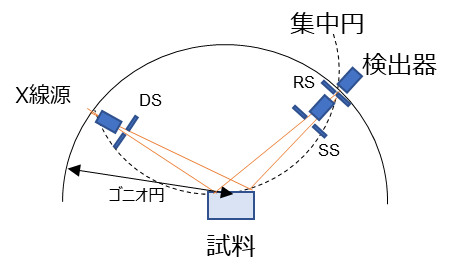
\includegraphics[scale=1.3]{XRD_theta_2theta_光学系.png}
				\caption{集中法光学系}
				\label{集中法光学系}
			\end{figure}

			\subsubsection{Pole figure測定}
			$\theta-2\theta$測定は試料表面に平行な格子面を測定するため、
			結晶面の逆格子ベクトル$\bm{g}_{hkl}$は常に試料の表面に垂直方向を向いている。
			逆格子ベクトル$\bm{g}_{hkl}$の大きさは結晶面の間隔$d$の逆数$1/d$に対応しており、
			$\theta-2\theta$測定は結果的に様々な$d$値の格子面を観測する。
			$\theta-2\theta$測定においても試料の配置を変更するなどによって配向の有無程度は判断可能である。
			しかし配向度などの定量な詳しい評価はPole figure測定などが必要になる。
			
			Pole figure測定(別名:極点測定)は$\theta-2\theta$測定における回折角度$2\theta$を固定し、
			試料を回転、あおりを行い回折強度を測定する手法である。測定する回折面は固定されているため図\ref{極点の測定方法}の通り
			、$\bm{g}_{hkl}$の長さは一定となる。試料を$\alpha$(あおり)と$\beta$(面内回転)という
			2つの優先方位軸を用いて、回折角度一定の半球をスキャンする。
			計測結果は図\ref{極点の測定方法}(B)の通り、極図形を用いて表現する。
			配向度は図\ref{極点の測定方法}(C)の通り、得られた極座標を半径方向に積分し、以下の式\eqref{orientation}に基づいて計算される。
			\begin{equation}
				配向度 = \frac{360 - \sum ピークの半値幅 }{360}\times 100
				\label{orientation}
			\end{equation}
			\begin{figure}[h]
				\centering
				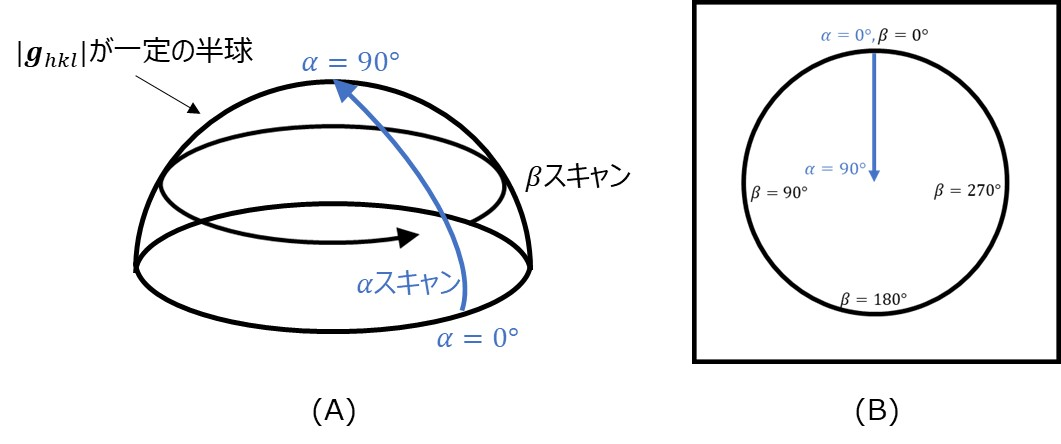
\includegraphics[width=\linewidth]{極点の測定方法.jpg}
				\caption{Pole figure測定の概念図. (A)逆格子ベクトルの大きさが一定により作られる半球におけるスキャン方向, 
				(B)極図形, (C)極図形の$\beta$依存性.}
				\label{極点の測定方法}
			\end{figure}
			\newpage
			Pole figure測定には図\ref{Pole_figure_outplane}のアウトプレーンの測定と図\ref{Pole_figure_inplane}のインプレーンの測定が存在する。
			アウトプレーンは試料に対するあおりを試料台を傾けて実現する。
			よって、$\alpha=0^{\circ}$近傍においては試料の側面に入射されてしまうため測定が困難になる。
			結果的にアウトプレーンの想定では$\alpha=0^{\circ}\sim90^{\circ}$の全極点測定は実質不可能である。
			インプレーンのPole figure測定は図\ref{Pole_figure_inplane}の通り、
			試料台を傾けず受光部を傾けてあおり$\alpha$を実現する。
			光学系においては図\ref{XRD_配置}の$2\theta$軸に直行する軸である$2\theta_\chi$軸を利用する。
			インプレーンのPole figure測定で$\alpha=0$は低角で測定する薄膜法を同様の状況であるため、
			薄膜法で使用する光学素子を使用する。例えば、集中光学法では集中発散ビーム(BB)を使用するが
			Pole figure測定では薄膜法で使用される平行ビーム(PB)を使用する。
			本研究においてはPole figure測定が可能であるSmart lab(Rigaku Corporation)を使用した。
			
			\begin{figure}[h]
				\centering
				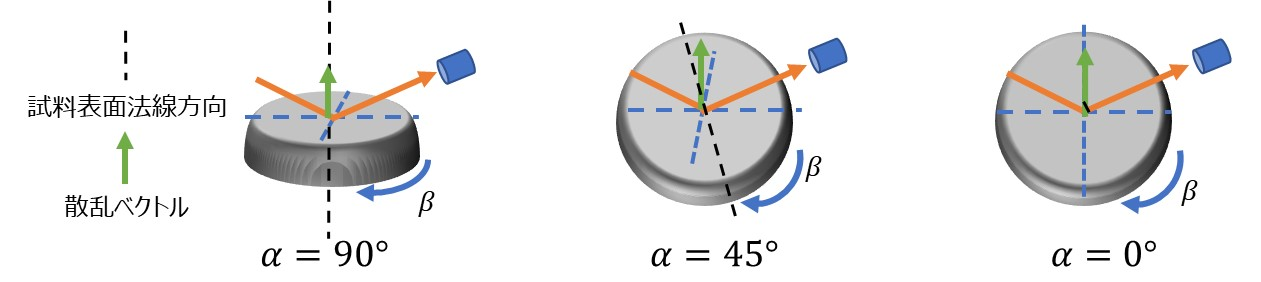
\includegraphics[width=0.9\linewidth]{pole_figure_outplane.jpg}
				\caption{アウトプレーンのPole figure測定.}
				\label{Pole_figure_outplane}
			\end{figure}
			\begin{figure}[h]
				\centering
				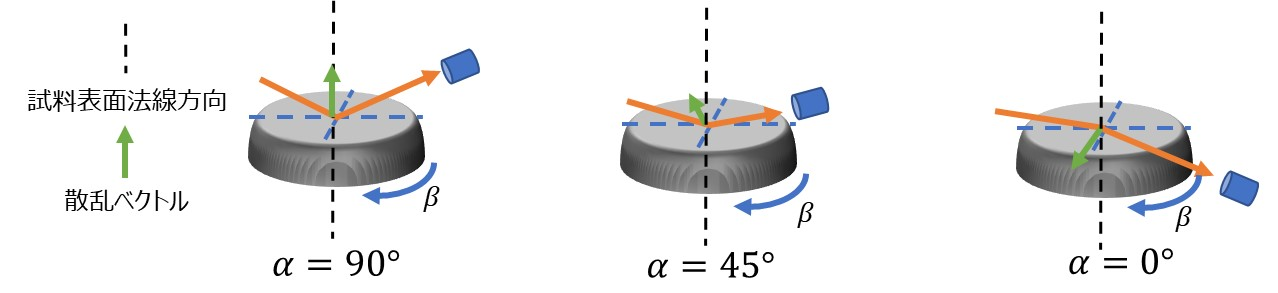
\includegraphics[width=0.9\linewidth]{pole_figure_inplane.jpg}
				\caption{インプレーンのPole figure測定.}
				\label{Pole_figure_inplane}
			\end{figure}
			\begin{figure}[h]
				\centering
				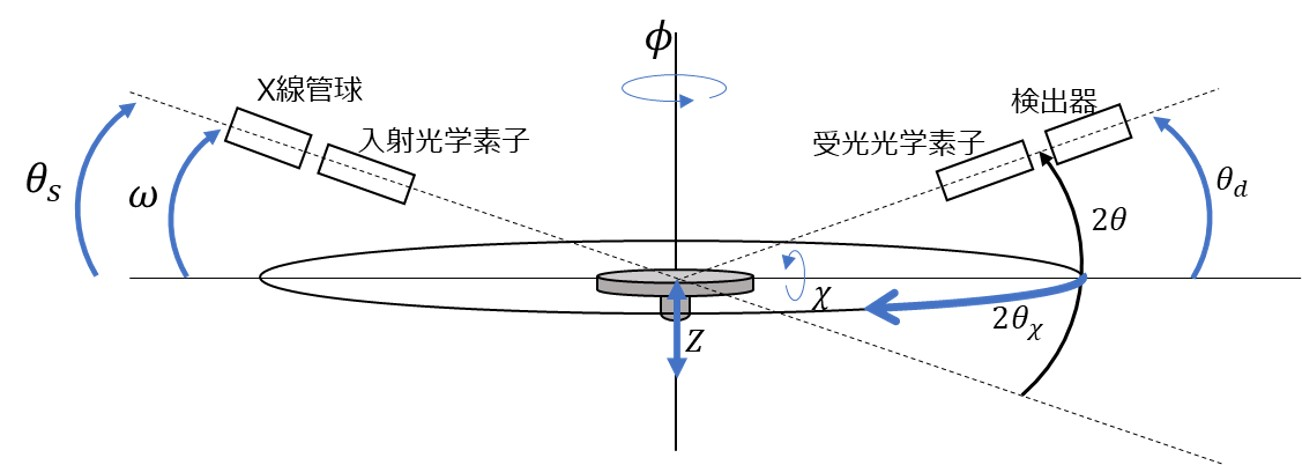
\includegraphics[width=0.9\linewidth]{XRD_配置.jpg}
				\caption{XRDの測定系.}
				\label{XRD_配置}
			\end{figure}
			\newpage
			\begin{figure}[h]
				\centering
				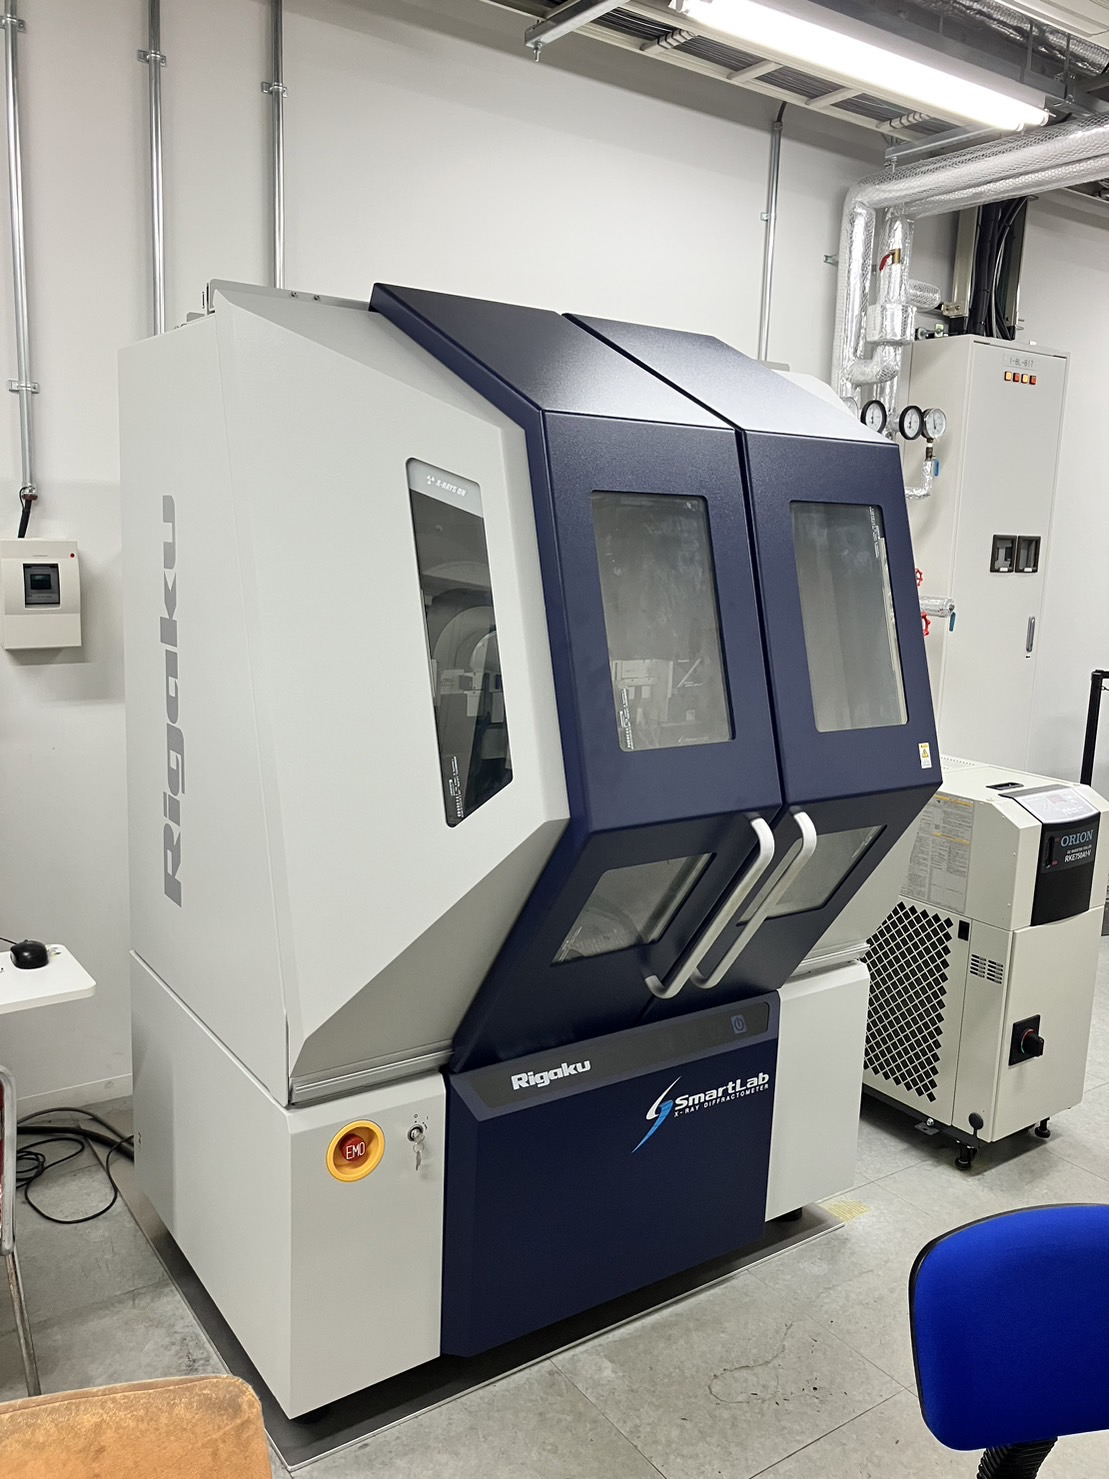
\includegraphics[width=0.5\linewidth]{smartlab.jpg}
				\caption{Pole figure測定に用いたXRD(Rigaku corporation).}
				\label{XRD_pole_figure}
			\end{figure}
			\newpage
			\subsection{誘電率測定}
			作製したシルクフィブロインフィルムの誘電率はインピーダンスアナライザ
			図\ref{インピーダンスアナライザ}(KEYSIGHT 4294A)を用いて測定した。
			圧電性の評価においては誘電率に現れる圧電性による効果を圧電共鳴法に基づいて評価した。
			\begin{figure}[h]
				\centering
				\begin{minipage}{0.45\hsize}
					\centering
					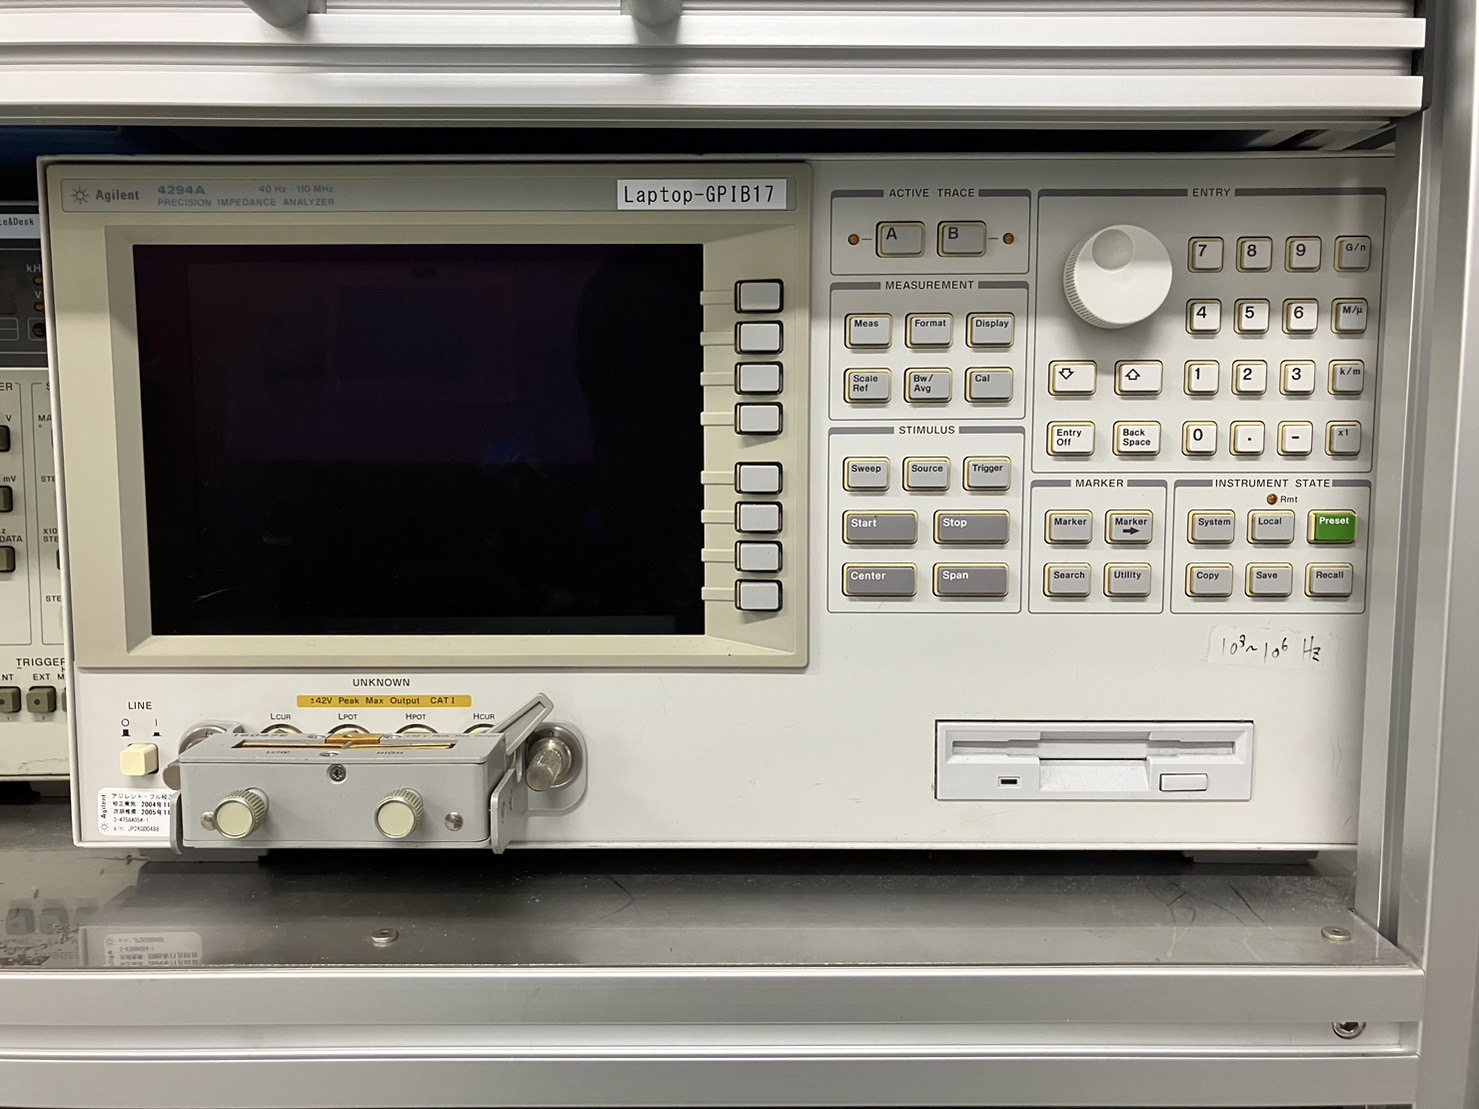
\includegraphics[width=\linewidth]{4294A.jpg}
					\caption{KEYSIGHT 4294A}
					\label{インピーダンスアナライザ}
				\end{minipage}
				\begin{minipage}{0.45\hsize}
					\centering
					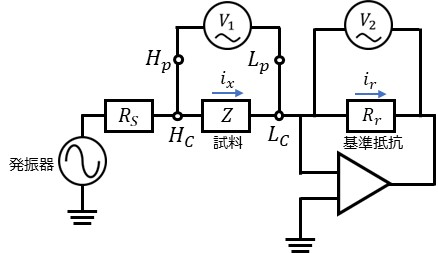
\includegraphics{自動平衡ブリッジ回路.jpg}
					\caption{自動平衡ブリッジ回路}
					\label{自動平衡ブリッジ回路}
				\end{minipage}
			\end{figure}
			\subsubsection{誘電率測定の原理}
			インピーダンスアナライザは自動平衡ブリッジ回路で構成されており図\ref{自動平衡ブリッジ回路}の通りである。
			自動平衡ブリッジ回路は試料に印加される電圧を計測する交流電圧計$V_1$と、
			試料を流れる電流を算出するために用いる交流電圧計$V_2$から構成されている。
			また、交流電圧計$V_1$は四端子測定が行われている。
			図\ref{自動平衡ブリッジ回路}における$L_C$はオペアンプの仮想短絡により0 Vである。
			オペアンプの高インピーダンス特性により、試料を流れる電流$i_x$と$i_r$は等価とみなせる。
			$i_r$は以下の式の通り、交流電圧計$V_2$を用いて計算できる。
			\begin{equation}
				i_r=i_x=-\frac{V_2}{R_r}
			\end{equation}
			試料に印加される電圧$V_1$と試料を流れる電流$i_x$を用いて以下の式のように、
			試料のインピーダンス$Z$を算出できる。
			また、式\eqref{impedance}における$R$はレジスタンス、$X$はリアクタンスである。
			\begin{equation}
				Z=\frac{V_1}{i_x}=\frac{V_1}{i_r}=-\frac{V_1}{V_2}R_r = R + j X  
				\label{impedance}
			\end{equation}
			式\eqref{impedance}よりインピーダンス$Z$は基準抵抗$R_r$と交流電圧比$V_1/V_2$から求まる。
			交流電圧比$V_1/V_2$はロックインアンプを用いて計算されるため、
			インピーダンスの大きさ$|Z|=|V_1 R_r/V_2|$と位相(Phase)$\phi$が出力される。
			その二つをもちいるとレジスタンス$R$とリアクタンス$X$の値も以下の式で計算される。
			\begin{equation}
				R = |Z| \cos \phi
			\end{equation}
			\begin{equation}
				X = |Z| \sin \phi
			\end{equation}
			またアドミッタンスはインピーダンスの逆数であるため式\eqref{admittance}のように決まる。
			式\eqref{admittance}における$G$はコンダクタンス、$B$はサセプタンスである。
			\begin{equation}
				Y= \frac{1}{Z}=-\frac{V_2}{V_1}\frac{1}{R_r} = G + j B
				\label{admittance}
			\end{equation}
			コンダクタンス$G$、サセプタンス$B$はロックインアンプにより出力される
			インピーダンスの大きさ$|Z|$と位相$\phi$を用いて以下のように計算される。
			\begin{equation}
				G = \frac{1}{|Z|} \cos \left(-\phi\right) = \frac{1}{|Z|} \cos \phi
				\label{コンダクタンス}
			\end{equation}
			\begin{equation}
				B = \frac{1}{|Z|} \sin(-\phi) = \frac{-1}{|Z|}\sin \phi
				\label{サセプタンス}
			\end{equation}

			測定試料が高インピーダンスな誘電体であり、
			測定する周波数区間が40 Hz -110 MHzであるため、
			測定試料の等価回路として抵抗$R_s$とコンデンサ$C_s$の並列モデルを採用する。
			このとき、アドミッタンス$Y_s$は以下のように記述できる。
			\begin{equation}
				Y_s = \frac{1}{R_s}+j\omega C_s
				\label{Y_s}
			\end{equation}
			一方、測定試料を理想的なコンデンサとみなすとき、そのアドミッタンスは試料の寸法
			(厚さ$d$, 電極面積$S$)を用いて以下のように求められる。
			\begin{equation}
				Y_p= j \omega C_p = j \omega \varepsilon^{*} \frac{S}{d} = 
				j\omega (\varepsilon'-j\varepsilon'')\frac{S}{d} =
				\omega\varepsilon''\frac{S}{d} + j\omega \varepsilon' \frac{S}{d}
				\label{Y_p}
			\end{equation}
			式\eqref{Y_s}の$Y_s$と式\eqref{Y_p}の$Y_p$は等価であるため、
			誘電率の実部$\varepsilon'$と虚部$\varepsilon''$は以下のように記述できる。
			\begin{equation}
				\varepsilon' = C_s \frac{d}{S}
				\label{real_epsilon}
			\end{equation}
			\begin{equation}
				\varepsilon'' = \frac{d}{\omega R_s S}
				\label{imaginary_epsilon}
			\end{equation}
			これより、インピーダンスアナライザを用いてインピーダンスの大きさ$|Z|$
			と位相$\phi$を計測し
			式\eqref{コンダクタンス}、式\eqref{サセプタンス}、式\eqref{Y_s}から
			抵抗$R_s$とコンデンサ$C_s$の値を求める。
			そして式\eqref{real_epsilon}と式\eqref{imaginary_epsilon}から
			誘電率の実部虚部を計算する。
			
			高周波においては誘電体のインピーダンスが小さくなる。
			誘電体表面に作製した電極のインピーダンスが、誘電体のインピーダンスに対して相対的に影響が大きくなる。
			等価モデルはコンデンサと抵抗の並列モデルではなく、抵抗とコンデンサの直列モデルが妥当となる場合がある。
			高周波においてもインピーダンスアナライザを用いた計測を行う場合、
			電極の抵抗を低くするなど工夫が必要である。
			
			本研究において圧電性の評価は誘電率を測定し、誘電率に現れる圧電共鳴成分を用いて評価
			する圧電共鳴法を用いた。
			フィッティングに用いた関数は式\eqref{normal_piezo_resonance}であるが
			$k_l=0, k_w=0$とし、$t\rightarrow l, f_t \rightarrow f_R$にして以下のように近似すると
			式\eqref{ずりの圧電共鳴_理論式}が得られる。
			\begin{equation}
				\varepsilon_{33} =
				\varepsilon_{33}^S
				\frac{1}{1-k_l^2\frac{\tan{\pi f/2f_R}}{\pi f/2f_R}}
				= \varepsilon_{33}^S\left(1-k_l^2\frac{\tan{\pi f/2f_R}}{\pi f/2f_R}\right)^{-1}
				\approx \varepsilon_{33}^S\left(1+k_l^2\frac{\tan{\pi f/2f_R}}{\pi f/2f_R}\right)
			\end{equation}
			また、フィッティングに式\eqref{normal_piezo_resonance}を用いているため、
			弾性率は2倍大きく、圧電$e$定数は$\sqrt{2}$倍大きく、圧電$d$定数は$1/\sqrt{2}$倍
			小さく求められるため、フィッティングした後に修正した。
			そして長さ方向と幅方向のどちらにおいても計測対象が$k_{14}$の1つであるため
			本研究では試料の寸法は正方形とした。
			\newpage
			\section{原子間力顕微鏡(AFM), 圧電応答顕微鏡(PFM)}
			原子間力顕微鏡(AFM)、圧電応答顕微鏡(PFM)はどちらも走査型プローブ顕微鏡(SPM)に属する。
			走査型プローブ顕微鏡(SPM)とは、微小な深針(カンチレバー)で試料をなぞり、
			その形状や物性を観察、計測する顕微鏡の総称である。図\ref{SPM}, \ref{cantilever_photo_detector}
			にSPMの基本構成を示す。SPMに属する顕微鏡は図\ref{SPM}のように
			カンチレバーを試料表面に接触または接近させて、走査中に生じる試料のある物理量の変化を検出する。
			本研究にて用いるSPMは原子間力顕微鏡(AFM)と圧電応答顕微鏡(PFM)のみである。
			この二つにおいては、図\ref{cantilever_photo_detector}のようにそれぞれの物理量変化
			によってカンチレバーがたわみ、そのカンチレバーに照射したレーザーの変位を
			フォトディテクターで計測し、測定対象の物理量変化を測定する。
			つまり、レーザーの変位から物質表面の物性変化をみる。
			原子間力顕微鏡(AFM)はカンチレバーと試料間に生じる原子間力を検出し
			試料表面画像を取得する。圧電応答顕微鏡(PFM)は試料の逆圧電効果に
			よる表面の歪みをカンチレバーの変位として取得し画像化する。
			\begin{figure}[h]
				\centering
				\begin{minipage}{0.45\hsize}
					\centering
					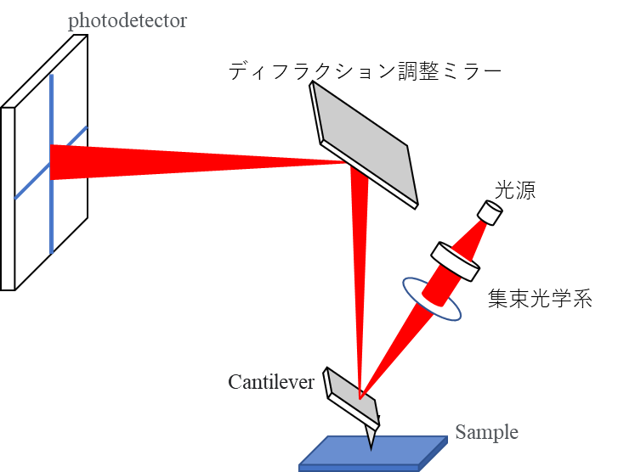
\includegraphics[width=\linewidth]{SPM.png}
					\caption{走査型顕微鏡(SPM)の光学系}
					\label{SPM}
				\end{minipage}
				\begin{minipage}{0.45\hsize}
					\centering
					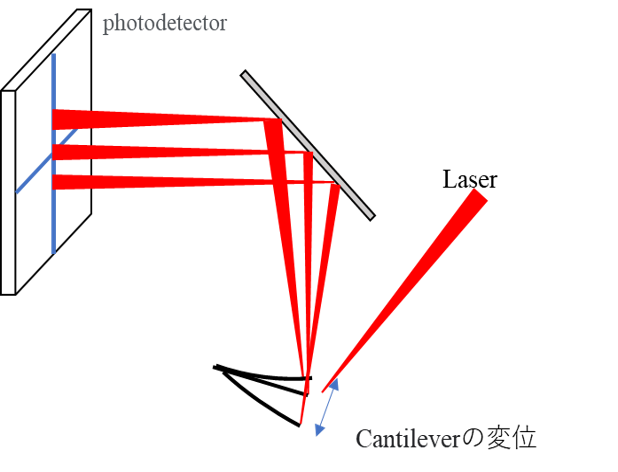
\includegraphics[width=\linewidth]{SPM2.png}
					\caption{CantileverとPhotodetectorの関係}
					\label{cantilever_photo_detector}
				\end{minipage}
			\end{figure}
				\subsubsection{AFM(Atomic Force Microscopy)}
				\begin{figure}[h]
					\centering
					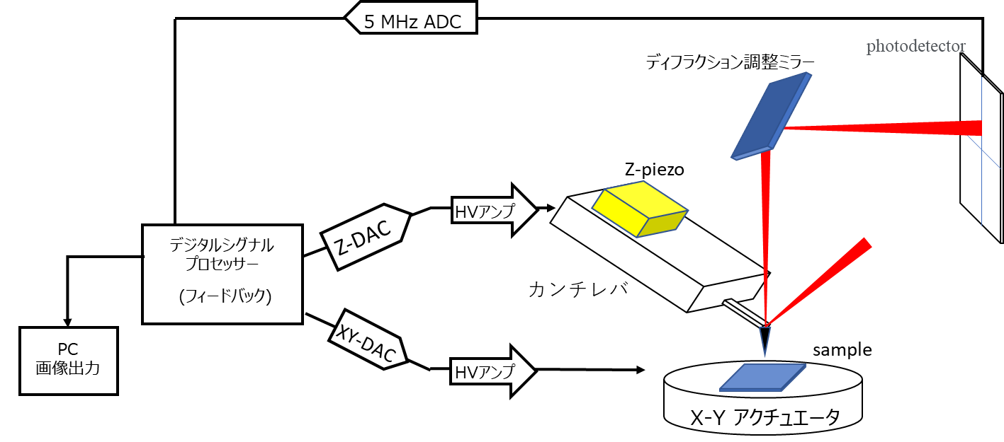
\includegraphics[width=0.8\linewidth]{AFM.png}
					\caption{AFMの信号模式図}
					\label{stracture_of_AFM}
				\end{figure}
				図\ref{stracture_of_AFM}はAFMの信号模式図である。AFMの測定手法にはタッピングモード(ACモード)
				とコンタクトモード(DCモード)がある。タッピングモードは、カンチレバーを内部に存在する圧電素子を用いて
				共振周波数で振動させ、試料表面を断続的に接触させながら走査する。測定対象の表面形状からカンチレバーの振動振幅が変動し、
				画像化する。正確にはカンチレバーを試料表面に近づけると原子間力を検出し、
				この瞬間カンチレバーの振動振幅は小さくなる。この振動振幅の変位をレーザーの変位として取得し、
				この変位分だけ元に戻すようにフィードバックをかけ、Z軸方向をZピエゾで調整する。このZピエゾの変位を画像化し、表面像を得る。
				コンタクトモードはタッピングモードと異なり、
				カンチレバーを振動させずに静的な状態で試料に常に接触させながら試料表面を走査し、
				表面の凹凸に対応したカンチレバーのたわみをレーザーの変位としてフォトディテクターから検出する。
				このレーザーの変位を一定にするようにZピエゾを用いて、フィードバック制御を行う。そのZピエゾの変位を表面形状として画像化する。
				本研究において、AFMを用いた計測はカンチレバーの消耗の観点からタッピングモードで行った。
				\subsubsection{PFM(Piezoresponse Force Microscopy)}
				走査型プローブ顕微鏡(Scanning Prob Microscope, SPM)の一種として圧電応答顕微鏡
				(Piezoresponse Force Microscopy, PFM)がある。
				圧電応答顕微鏡(PFM)は試料の逆圧電効果による表面の歪みをカンチレバーの変位として取得し画像化する顕微鏡である。
				図\ref{PFMの概念図}のように試料片面基板からカンチレバー間で交流電場を印加する。
				このとき試料の分極方向に依存して、電場の変化に対応した歪みが試料に生じる。
				その歪の大きさはカンチレバーの変位の大きさとして現れ、
				Amplitude像として取得できる。
				\begin{figure}[h]
					\centering
					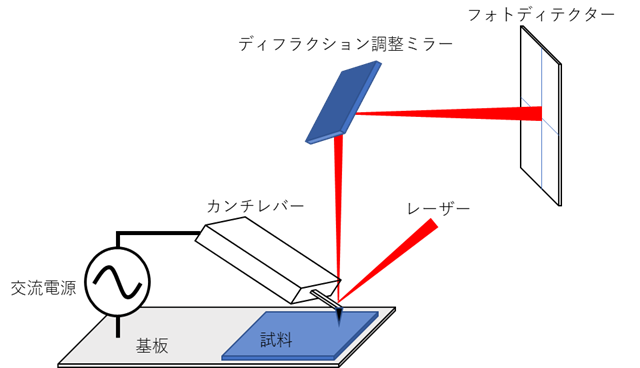
\includegraphics{PFM.png}
					\caption{PFMの概念図}
					\label{PFMの概念図}
				\end{figure}
				\\
				また、図\ref{PFM_phaseの概念図}のように交流電場に対応した試料の歪み方向は試料中の分極方向に依存しているため、
				この分極方向を交流電場と歪みの位相差から解析し、Phase像として取得できる。
				\begin{figure}[h]
					\centering
					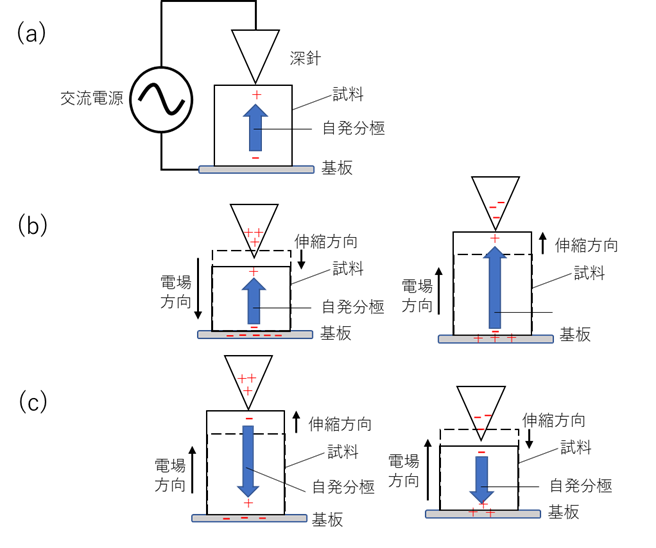
\includegraphics[width=0.8\linewidth]{PFM_phase.png}
					\caption{PFMのPhase像概念図. (a)電場E=0の様子,
					(b)交流電場と試料の伸縮方向が同位相であるときの自発分極方向, 
					(c)交流電場と試料の伸縮方向が逆位相であるときの自発分極方向.}
					\label{PFM_phaseの概念図}
				\end{figure}
				PFMはカンチレバーを試料上に接触させ走査するコンタクトモードで行われる。
				カンチレバーと試料からの相互作用を加味した共振周波数、
				コンタクト周波数でカンチレバーを振動させることで、
				その振動振幅の変化から、より高精度に圧電応答を観察できるようになっている。
				しかし、そのコンタクト周波数は走査中一定に保たれているわけではない。
				なぜならば、走査中の試料表面の形状変化によるカンチレバーの接触面積の違いがコンタクト周波数をシフトさせる要因になる。
				コンタクト周波数のシフトにより、圧電応答によるカンチレバーのたわみ変化の大きさと走査中における試料表面の形状変化によるカンチレバーのたわみ変化がクロストークしてしまい、
				正確な圧電応答や表面像を取得できなくなる。よって測定材料は測定前に表面を平らにする必要がある。
				
				図\ref{PFM_phaseの概念図}は垂直方向のみでの議論である。しかし、図\ref{PFMの概念図}におけるフォトディテクターから分かる通り、
				図\ref{面内と垂直の概念図}の様に試料の面内方向の圧電性の評価も可能である。本研究においてはずり圧電の評価にて使用した。
				\begin{figure}[h]
					\centering
					
\includegraphics[scale=0.7]{lateral_vertical.png}
					\caption{カンチレバーにおける面内方向(Lateral)と垂直方向(Vertical)の関係.}
					\label{面内と垂直の概念図}
				\end{figure}
				\newpage
				生体材料の一つであるコラーゲンの圧電行列は以下の通りである。
				\begin{equation}
					\left(
				\begin{array}{cccccc}
					0&0&0&d_{14}&d_{15}&0 \\
					0&0&0&d_{15}&-d_{14}&0 \\
					d_{31}&d_{31}&d_{33}&0&0&0
				\end{array}\right)
			\end{equation}
				コラーゲン繊維の側面において面内PFM、コラーゲン繊維の断面において垂直PFMを行った報告がある\cite{コラーゲン繊維PFM}。
				このように生体材料の圧電測定においてPFMは頻繁に利用されている。
				\begin{figure}[ht]
					\begin{center}
					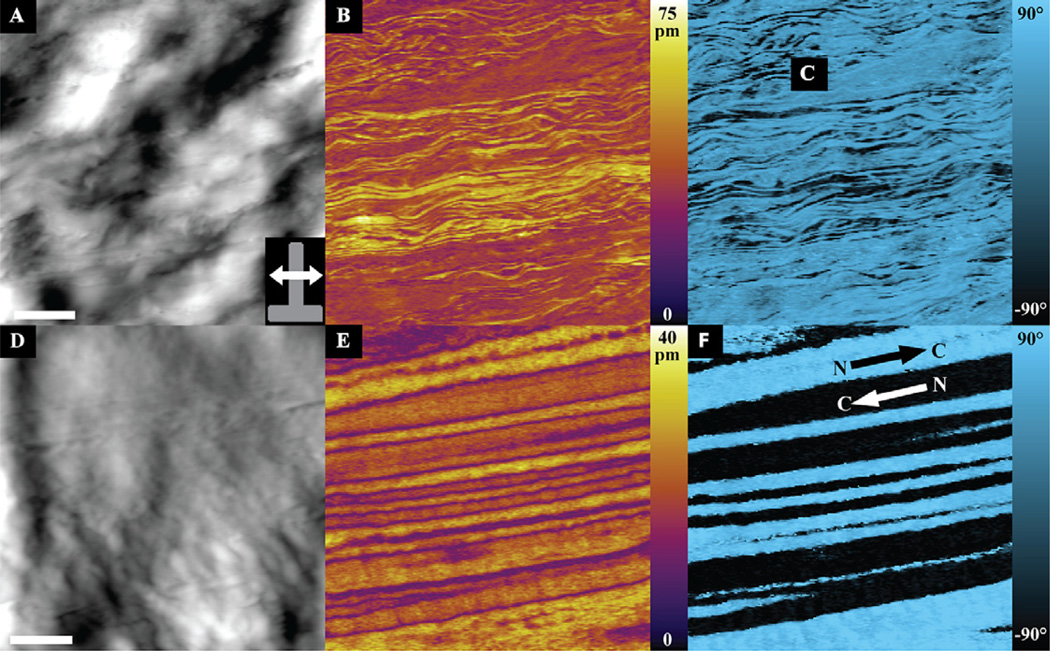
\includegraphics[scale=0.6]{PFM_コラーゲン_側面.jpg}
					\caption{コラーゲン繊維(側面)での面内PFM\cite{コラーゲン繊維PFM}.
					(A) AFM topology, (B) 面内PFM, (C) 面内PFMのPhase, 
					(D) AFM topology, (E) 面内PFM, (F) 面内PFMのPhase.
					(A)-(C)のスケールバーは2 {\textmu}m, 
					(D)-(F)のスケールバーは200 nm.}
					\label{PFM_コラーゲン_側面}
					\end{center}
				\end{figure}
				\begin{figure}[h]
					\centering
					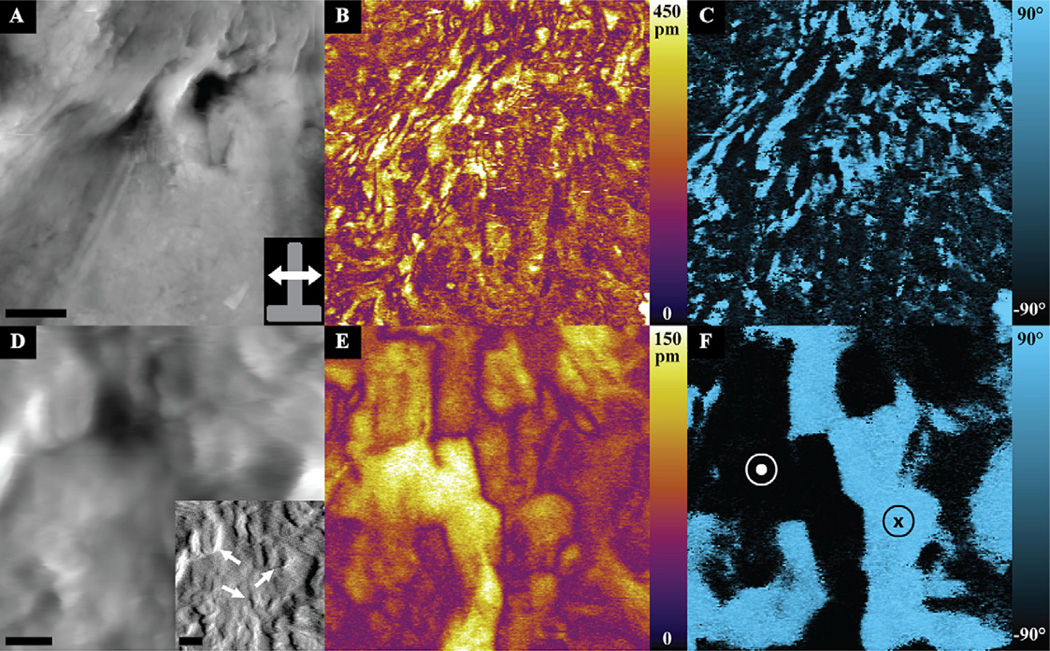
\includegraphics[scale=0.6]{PFM_コラーゲン_断面.jpg}
					\caption{コラーゲン繊維(断面)での垂直PFM\cite{コラーゲン繊維PFM}.
					(A) AFM topology, (B) 垂直PFM, (C) 垂直PFMのPhase
					, (D) AFM topology, (E) 垂直PFM, (F) 垂直PFMのPhase.
					(A)-(C)のスケールバーは2 {\textmu}m, 
					(D)-(F)のスケールバーは200 nm.}
					\label{PFM_コラーゲン_断面}
				\end{figure}
				\newpage
	\chapter{構造評価}
			\section{様々な種類のシルクのXRD($\theta$-$2\theta$)}
			図\ref{様々な絹糸XRD}は家蚕(Bombyx mori)、エリ蚕(Samia cynthia ricini)、
			サク蚕(Antheraea pernyi)の糸におけるXRDの$\theta$-$2\theta$測定の結果である。
			家蚕は$2\theta \approx 10^{\circ}, 20^{\circ}, 28^{\circ}$においてピークが伺える。
			エリ蚕は$2\theta \approx 16.5^{\circ}, 20^{\circ}$においてピークが伺える。
			サク蚕もエリ蚕と同様の位置にピークが確認されるが強度比が異なる。
			サク蚕、エリ蚕のどちらも家蚕と同じ逆平行$\beta$シートであるが、
			家蚕の方が単位格子が正方晶に近いため回折線が重なって見える\cite{warwicker1954}。
			\begin{figure}[h]
				\centering
				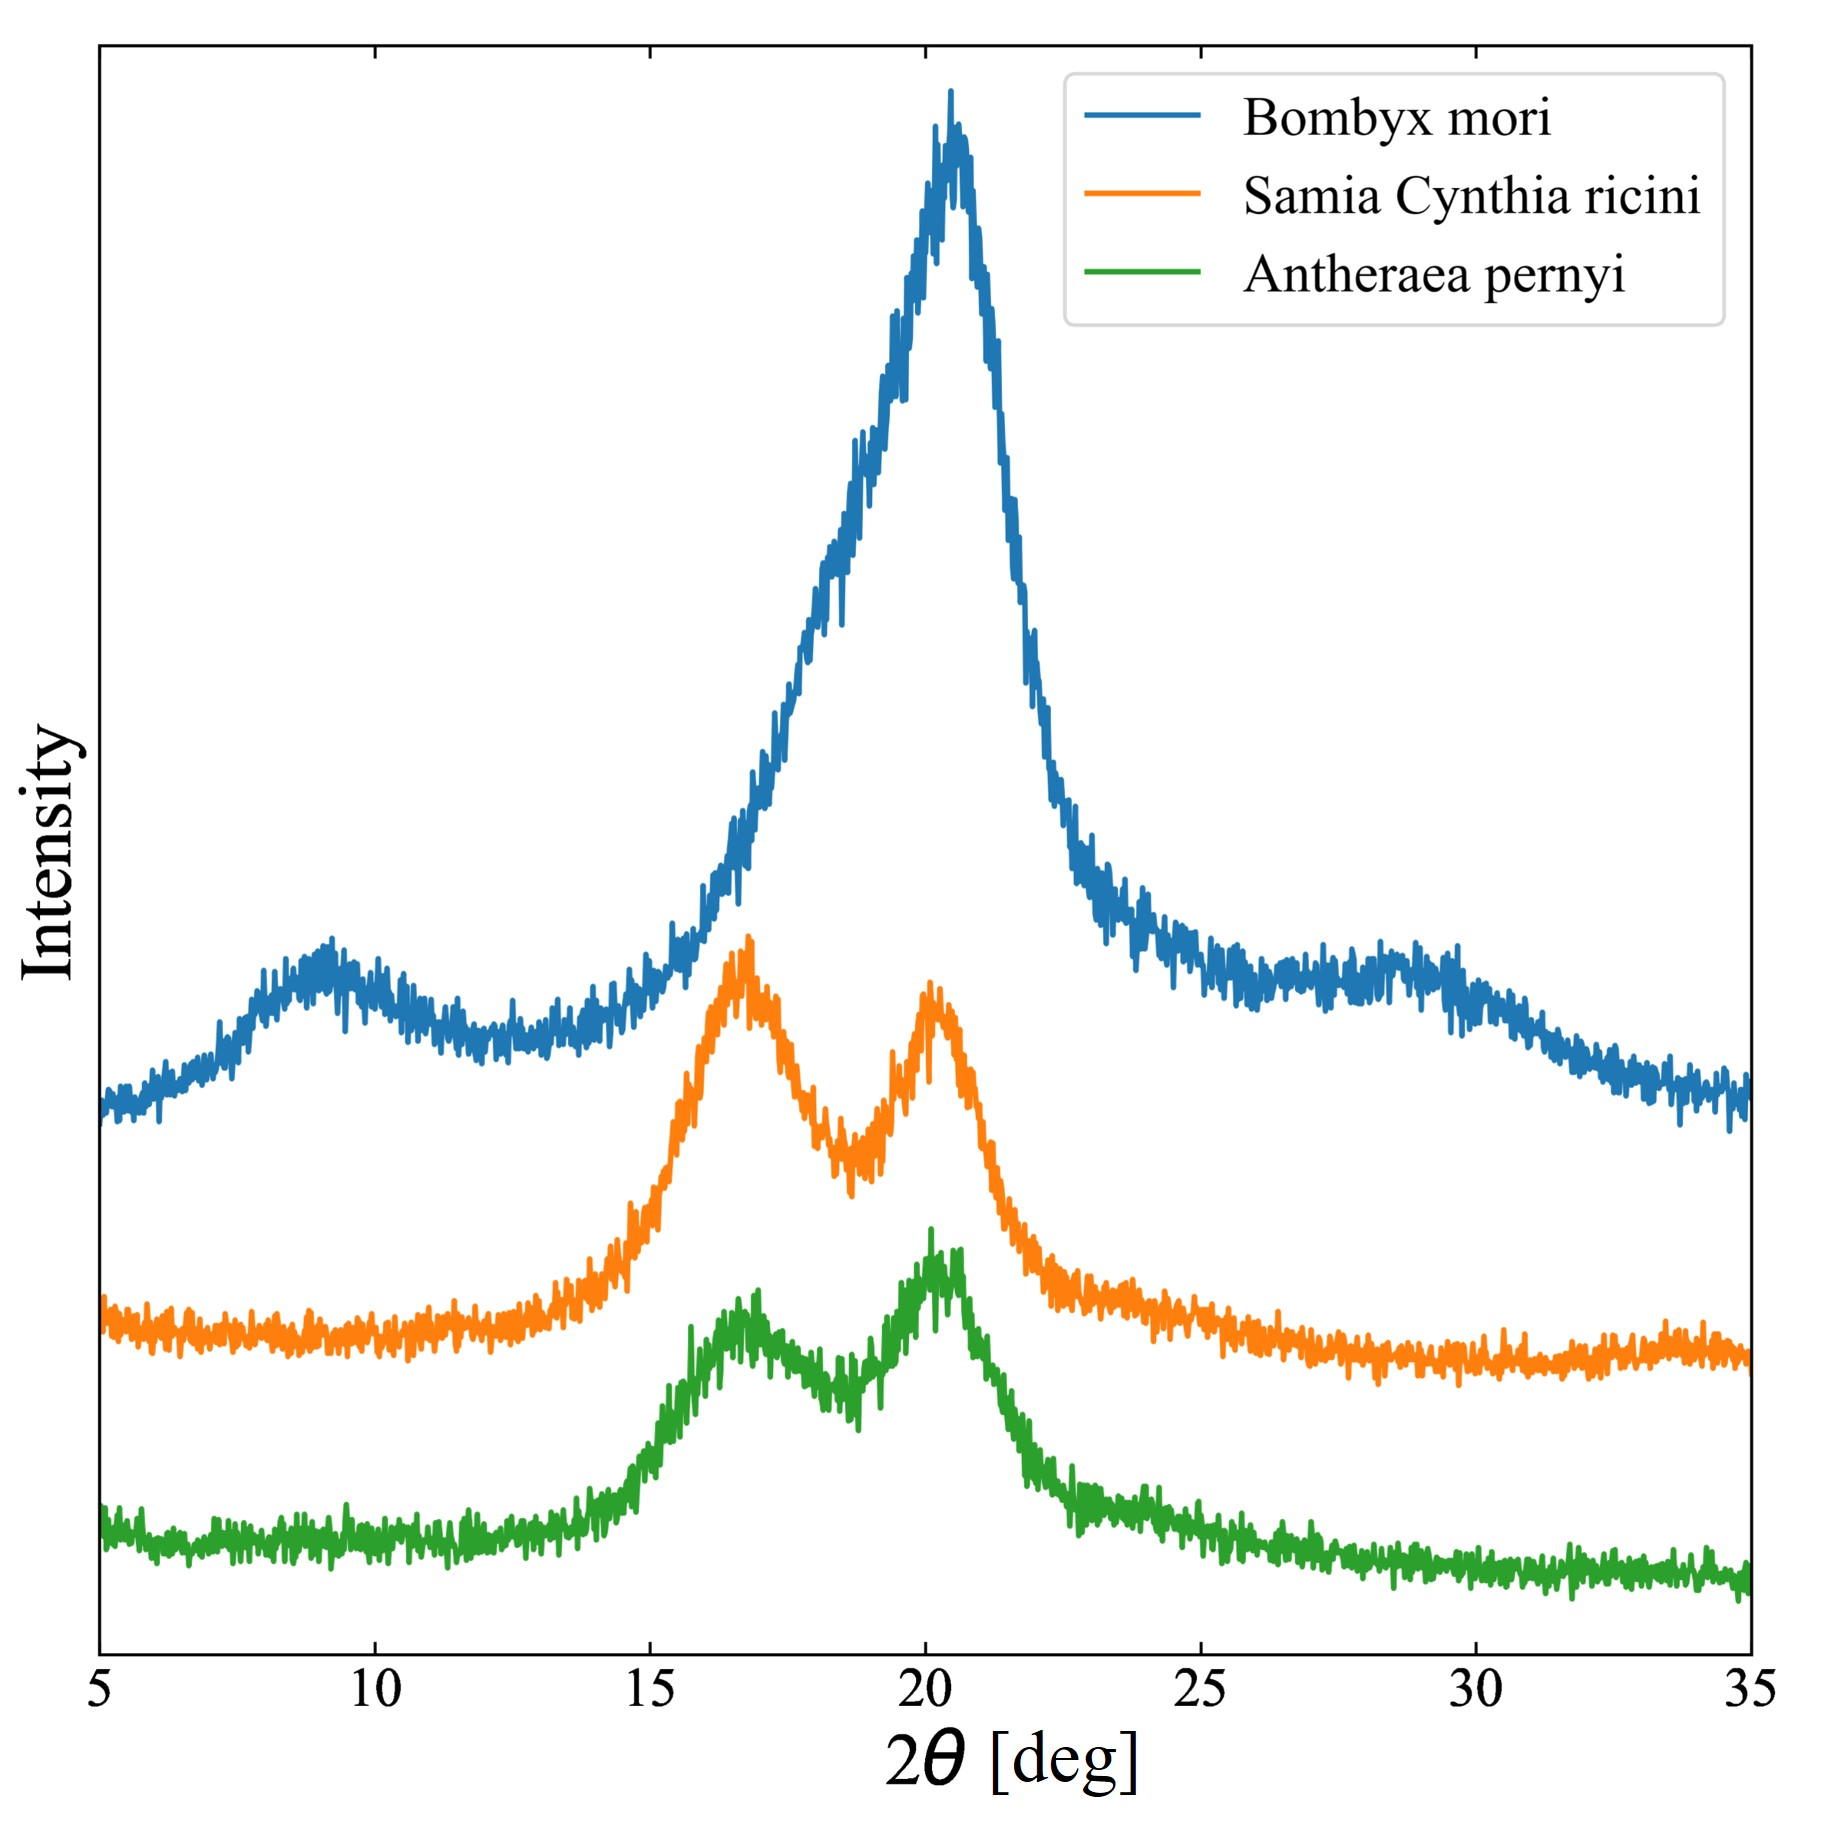
\includegraphics[scale=0.8]{糸の種類別XRD.jpg}
				\caption{家蚕(Bombyx mori), エリ蚕(Samia cynthia ricini), 
				サク蚕(Antheraea pernyi)の$\theta$-$2\theta$測定の結果.}
				\label{様々な絹糸XRD}
			\end{figure}
			\newpage
			\section{家蚕(Bombyx mori)におけるX線回折と配向性評価}
			図\ref{theta_2theta_fibroin_film}がセリシンを除去した
			シルクフィルムにおいて糸を並べた平行方向(parallel)と
			垂直方向(vertical)の$\theta - 2\theta$測定を行った結果である。
			silk IIのピーク\cite{marshモデル}とされる$2\theta = 10^{\circ}, 20^{\circ}, 29^{\circ}$付近にピークが確認された。
			vertical方向とparallel方向で大きな違いは見られなかった。
			
			$\theta - 2\theta $測定にて最も大きなピークが表れた$2\theta=20^{\circ}$にて
			pole figure測定を行い、結果が図\ref{極点図_結果_without_sericin}である。
			図\ref{極点図_結果_without_sericin}(A)が極点図であり、
			(B)が極点図を半径方向に積分した結果である。
			90°、270°方向を糸を並べた方向(parallel)としたため、
			作製したフィルムの配向軸は糸を並べた方向(parallel)と判明した。
			$\theta-2\theta$測定の結果と大きく異なるが、これは$\theta-2\theta$測定
			が試料の垂直方向の結晶面間隔しか評価されないためと思われる。
			図\ref{極点図_結果_without_sericin}(B)において半値幅から配向度
			を計算すると88\%となった。

			セリシンを含むシルクフィルムにおける$\theta -2\theta$測定は図\ref{セリシン含む_theta_2theta}
			である。$2\theta \approx 10^{\circ}$付近の違いがあるものの、$2\theta \approx 20^{\circ}$
			のピークでは強度の違いは生まれなかった。
			図\ref{セリシン含む_pole_figure}は$2\theta = 20^{\circ}$で測定した
			セリシン含むシルクフィルムにおけるpole figureの極点図と極点図を半径方向に積分した結果である。
			配向度は77\%となり、セリシンを含まない場合より低い値となったが結晶面が配向していると思われる。
			\begin{figure}[H]
				\centering
				\includegraphics[scale=0.8]{theta_2theta_fibroin_film}
				\caption{セリシンを除去したシルクフィルムの$\theta - 2\theta$測定の結果。
				parallelが並べた糸と平行方向、verticalが並べた糸と垂直方向。}
				\label{theta_2theta_fibroin_film}
			\end{figure}
			\newpage
			\begin{figure}[h]
				\centering
				\includegraphics[width=\linewidth]{pole_figure_silk_fibroin.jpg}
				\caption{セリシンを除去したシルクフィルムにおけるpole figure測定。(A)極点図、
				(B)極点図を半径方向に積分した結果。90$^{\circ}$、270$^{\circ}$を繊維軸(parallel)とした。}
				\label{極点図_結果_without_sericin}
			\end{figure}
			\begin{figure}[H]
				\centering
				\includegraphics[scale=0.75]{theta_2theta_セリシンあり.jpg}
				\caption{セリシンを含むシルクフィルムの$\theta - 2\theta$測定の結果。
				parallelが並べた糸と平行方向、verticalが並べた糸と垂直方向。}
				\label{セリシン含む_theta_2theta}
			\end{figure}
			\newpage
			\begin{figure}[h]
				\centering
				\includegraphics[width=\linewidth]{セリシンあり_polefigure.jpg}
				\caption{セリシンありのシルクフィルムにおけるpole figure測定。(A)極点図、
				(B) 極点図を半径方向に積分した結果。0$^{\circ}$、180$^{\circ}$を繊維軸(parallel)とした。}
				\label{セリシン含む_pole_figure}
			\end{figure}
			\subsection{$\theta-2\theta$の角度依存性}
			精錬したフィルムにおいて$\theta-2\theta$測定を
			360°試料を面内で回転させながら計測した。
			$\theta-2\theta$測定が試料の膜厚方向の結晶面しか計測されていないため
			配向したフィルムにおいてもデバイシェラー環の様な円環が得られたと思われる。
			\begin{figure}[H]
				\centering
				\includegraphics[scale=0.9]{デバイ.jpg}
				\caption{$\theta-2\theta$を試料に対して360°面内で計測した結果。
				(A)計測で得られた生データ、(B)logスケールに変換した結果。}
			\end{figure}
			\newpage
			\section{FTIR}
			作製したフィルムの蛋白質の二次構造の割合を知るためにFTIRを行った。
			測定した波数は400 cm$^{-1}$から4000 cm$^{-1}$とした。
			セリシンありのフィルムで実際に入手したデータを可視化すると
			図\ref{FTIR_セリシンあり}の通りである。
			\begin{figure}[h]
				\centering
				\includegraphics[scale=0.6]{FTIR_セリシンあり.jpg}
				\caption{セリシンありFTIRを行った結果}
				\label{FTIR_セリシンあり}
			\end{figure}
			\\
			セリシン除去過程を含まないフィルム、含むフィルム、それぞれを190℃で二時間の熱処理を行った場合の蛋白質、
			二次構造の割合は表\ref{FTIR_蛋白質二次構造}の結果にまとめた。
			また、表\ref{FTIR_蛋白質二次構造}における濃い黄色、薄い黄色とは図\ref{熱処理後のフィルム}
			の画像の通りである。
			熱処理前のセリシンあり、なしのフィルムにおいてセリシンなしの場合の方が最安定の$\beta$ シートが多い。
			これはセリシンを取り除く、炭酸ナトリウム水溶液の熱湯の浸水にて熱処理と同じ効果にて
			$\alpha$ helixが$\beta$ sheet へ転移したものによると思われる。
			190℃の二時間に渡る熱処理後ではどちらの場合でも$\beta$ sheetの含有量が増え、
			$\alpha$ helixが減った。セリシンありの薄い黄色の場合は異なるが、熱処理後のフィルムは
			$\alpha$ helixが1 \%まで減った。

			フィルムの特徴として熱処理後のフィルムは硬く、脆く、割れやすい。
			$\beta$ sheetが多い、濃い黄色の箇所は顕著である。
			\begin{table}[h]
				\centering
				\caption{FTIRによる蛋白質二次構造の割合の結果}
				\label{FTIR_蛋白質二次構造}
				\begin{tabular}{c c c c c} \hline
					フィルムの種類 & $\alpha$ helix & $\beta$ sheet &$\beta$ turn & other \\ \hline \hline
					セリシンあり(熱処理前) & 16 \% & 35 \% &  24 \% & 25 \% \\
					セリシンあり(熱処理後)、薄い黄色 &  12 \% & 39 \% & 4 \% & 25 \% \\
					セリシンあり(熱処理後)、濃い黄色 & 1 \% & 42 \% & 28 \% & 29 \% \\
					セリシンなし(熱処理前) & 8 \% & 48 \% &  21 \% & 23 \% \\
					セリシンなし(熱処理後)、薄い黄色 &  1 \% & 50 \% & 22 \% & 24 \% \\
					セリシンなし(熱処理後)、濃い黄色 & 1 \% & 54 \% & 24 \% & 23 \% \\ \hline
				\end{tabular}
			\end{table}
			\newpage
			\begin{figure}[h]
				\centering
				\includegraphics[scale=0.5]{シルクフィルム_熱処理後.jpg}
				\caption{190℃で熱処理した後のフィルム. (A) セリシンあり, (B) セリシンなし.}
				\label{熱処理後のフィルム}
			\end{figure}
			\newpage
			\section{AFM像, PFM像}
			図\ref{5_5_AFM_silk}、図\ref{1_1_AFM_silk}は
			市販されている(販売元不明)絹糸表面のAFM像である。
			表面に凹凸形状が確認できる。
			既に報告されているAFM像、図\ref{先行研究_AFM_糸}と同様にミクロフィブリルが確認された。
			\begin{figure}[h]
				\centering
				\includegraphics[width=\linewidth]{AFM_5_5.jpg}
				\caption{5 \si{\micro\meter}$\times$ 5 \si{\micro\meter}におけるAFM絹糸表面像. 
				(A) Topology, (B) Amplitude, (C) Phase. }
				\label{5_5_AFM_silk}
			\end{figure}
			\begin{figure}[h]
				\centering
				\includegraphics[width=\linewidth]{AFM_1_1.jpg}
				\caption{1 \si{\micro\meter}$\times$ 1 \si{\micro\meter}におけるAFM絹糸表面像. 
				(A) Topology, (B) Amplitude, (C) Phase.}
				\label{1_1_AFM_silk}
			\end{figure}
			\begin{figure}[H]
				\centering
				\includegraphics[scale=0.5]{AFM_silk.jpg}
				\caption{ミクロフィブリル\cite{クモと絹糸の構造}. (A)絹糸の構造, (B) AFM像におけるミクロフィブリル.}
				\label{先行研究_AFM_糸}
			\end{figure}
			\newpage
			市販の絹糸(販売元不明)のPFM像は図\ref{silk_fiber_PFM}の通りである。
			\begin{figure}[h]
				\centering
				\includegraphics[width=\linewidth]{PFM_silk_fiber.jpg}
				\caption{絹糸の垂直PFMと面内PFM. (A) Height, (B) 垂直Amplitude, (C) 垂直Phase, 
				(D) 面内Amplitude, (E)面内Phase.}
				\label{silk_fiber_PFM}
			\end{figure}
			\newpage
			\section{DSC}
		\label{DSC}
		熱特性を評価するために
		示差走査熱量測定(Differential Scanning Calorimetry; DSC)を使用した。
		DSCとは参照試料と測定試料を同じ温度で走査し、その熱量差を測定する。
		本研究ではDSC7020(Hitachi Corporation)を使用した。
		参照試料として空のアルミパンを使用した。
	
		糸の種類別の熱特性評価は図\ref{DSC熱特性評価}(A)の通りである。
		本研究にて使用したシルクは家蚕(Bombyx mori)である。他にも市販のエリ蚕(Samia cynthia ricini)、
		サク蚕(Antheraea pernyi)の糸の熱特性を評価した。
		家蚕とサク蚕の熱異常は73℃付近に表れている。
		よって本研究のシルクフィルムは73℃にてプレスして作製した。
		また、エリ蚕における熱異常のピークは他の糸と比べ高い97℃付近に表れた。
		図\ref{DSC熱特性評価}(B)は$-50$℃から$350$℃における家蚕のDSCを用いた熱特性である。
		図\ref{DSC熱特性評価}(A)に見られた73℃付近の熱異常は図\ref{DSC熱特性評価}(B)では90℃に移動している。
		これは蚕の個体差、あるいはサンプルの含水量の違いであり本質的に違いはないと思われる。
		よって図\ref{DSC熱特性評価}(A)におけるエリ蚕の熱異常温度の違いは蚕の個体差や含水量の違いによる
		可能性もある。
		同様に0℃付近における熱異常は水によるものと思われる。
		また、220℃付近に存在する熱異常はシルクの$\alpha$ ヘリックスから$\beta$シートに転移したものと思われる。
		300℃付近における大きな熱異常は分解によるものである。
		\begin{figure}[H]
			\centering
			\includegraphics[scale=0.75]{DSC_silk_0112_2.jpg}
			\caption{DSCによるシルクの熱特性評価. (A)家蚕(Bombyx mori), エリ蚕(Samia cynthia ricini), 
			サク蚕(Antheraea pernyi)の熱特性, (B)家蚕(Bombyx mori)の$-50$℃から$350$℃における熱特性.}
			\label{DSC熱特性評価}
		\end{figure}
		\newpage
		キャストフィルムに熱特性は図\ref{cast_film_DSC}の通りである。no treatmentが未延伸で熱処理を行っていない試料であり
		他は50℃、75℃、100℃、150℃で延伸を行った試料における熱特性である。
		図\ref{DSC熱特性評価}における糸の熱特性と異なりブロードな特性となった。
		しかし、50℃付近に見られる熱異常は延伸温度が100℃を超えると確認出来なくなったため、
		糸の場合と同様に水によるものと思われる。
		図\ref{cast_film_熱特性_DSC}は報告されているDSCを用いたフィブロインキャストフィルム
		の熱特性だが同様の結果は確認出来なかった。また、フィブロインキャストフィルム
		の作製方法は章\ref{キャストフィルムの作製方法}の通りである。
		\begin{figure}[h]
			\centering
			\includegraphics[scale=0.9]{cast_film_DSC_20210621.jpg}
			\caption{DSCをよるフィブロインキャストフィルムの熱特性}
			\label{cast_film_DSC}
		\end{figure}
		\begin{figure}[H]
			\centering
			\includegraphics[scale=1]{DSC_cast_film_report.jpeg}
			\caption{先行研究によるフィブロインキャストフィルムの熱特性\cite{cast_film_熱特性_DSC}}
			\label{cast_film_熱特性_DSC}
		\end{figure}
		\newpage
		図\ref{セリシン除去フィルムにおけるDSC}はセリシンを除去したシルクフィルムでDSCを用いて熱特性を計測した結果である。
		図\ref{セリシン除去フィルムにおけるDSC}(A)は計測した-150℃から350℃の全範囲での様子である。
		図\ref{セリシン除去フィルムにおけるDSC}(B)は温度を変えながら誘電率を測定した
		-70℃から120℃におけるDSCの結果である。
	
		図\ref{セリシンありフィルムにおけるDSC}はセリシンを残したシルクフィルムでDSCを用いて熱特性を計測した結果である。
		図\ref{セリシンありフィルムにおけるDSC}(A)は計測した-150℃から350℃の全範囲での様子である。
		図\ref{セリシンありフィルムにおけるDSC}(B)は温度を変えながら誘電率を測定した
		-70℃から120℃におけるDSCの結果である。
		セリシンを除去した場合と同様に80℃付近にブロードで分解と同程度の大きな吸熱ピークが伺える。
		また、300℃付近の分解も同様に確認される。セリシンを除去した場合に見られた-120℃, -40℃
		付近のピークは確認されなかった一方で、新たに0℃付近に発熱ピークが見られる。
		試料内部の水分であると思われる。また、セリシンを除去した場合において確認された40℃付近の吸熱ピークは
		確認されなかった。
		80℃の大きな吸熱ピークに隠れてしまったのか、元来、存在しないかは断定できない。
		ただし、圧電共鳴の弾性緩和を踏まえるとピークに隠れてしまったと考えるのが妥当だと思われる。
		セリシンを除去した場合、セリシンを残した場合のどちらにおいても220℃において吸熱ピークが存在する。
		190℃付近に存在すると報告されている、$\alpha$ ヘリックスから$\beta$シートへの転移によるものと思われる。
		\\
		\\
		\\
		\\
	
		\begin{figure}[h]
			\centering
			\includegraphics[width=\linewidth]{熱プレスシルクフィルム_DSC.jpg}
			\caption{セリシンを除去したシルクフィルムのDSCによる熱特性. (A) -150℃から350℃の熱特性, 
			(B) -70℃から120℃の熱特性.}
			\label{セリシン除去フィルムにおけるDSC}
		\end{figure}
		\begin{figure}[H]
			\centering
			\includegraphics[width=\linewidth]{セリシンあり_熱プレスシルクフィルム_DSC.jpg}
			\caption{セリシンを残したシルクフィルムのDSCによる熱特性. (A) -150℃から350℃の熱特性, 
			(B) -70℃から120℃の熱特性.}
			\label{セリシンありフィルムにおけるDSC}
		\end{figure}
		\section{TG-DTA}
		示差熱熱重量同時測定装置を用いて、シルクの温度と重量の関係、基準物質と温度差の関係を計測した。
		基準物質として空のPANを使用した。図\ref{TG_DTA}がその結果である。
		350℃付近にてTG曲線が落ち込んでおり、炭化である。また、計測時は解放PANであるため
		炭化済みであると確認した。50℃から250℃において緩やかにTG曲線が減少しているが
		脱水、結晶化など様々な現象を含んでいると思われる。
		\begin{figure}[H]
			\centering
			\includegraphics[scale=0.4]{TG_DTA.jpg}
			\caption{シルク(Bombyx)のTG-DTA曲線}
			\label{TG_DTA}
		\end{figure}
		\chapter{物性評価}
		\section{圧電共鳴の試料寸法と角度依存性}
		セリシンを除去したフィルムにおいて、1辺の大きさが5 mm, 7.5 mm, 10 mmである正方形試料を作製した。
		図\ref{45deg_cut_piezo_resonant}は45°カットでそれぞれの試料寸法における圧電共鳴スペクトルである。
		また、図\ref{0deg_cut_piezo_resonant}は0°カットでそれぞれの試料寸法における圧電共鳴スペクトルである。
		どちらの場合においても圧電共鳴は、100 kHz付近に観測された。
		同時に共鳴周波数の式\eqref{ずりの共鳴周波数}に対応して、正方形試料の
		1辺が大きいと低周波側に、1辺が小さいと高周波側に表れた。
		ずり圧電の原理上、0°カットの場合は圧電共鳴スペクトルは表れないと考えられるが
		異なる結果となった。
		共鳴周波数$f_r$から式\eqref{ずりの共鳴周波数}を用いて弾性率$c=1/s$は、試料寸法$l$、密度$\rho$
		として以下のように計算される。
		\begin{equation}
			c = \frac{1}{s} = 2l^2 f_R^2 \rho
		\end{equation}
		入手した圧電共鳴スペクトルに対し、式\eqref{ずりの圧電共鳴_理論式}に基づいてフィッティングした
		後に上式から弾性率を計算した。
		横軸を試料の切り出し角度、縦軸を弾性率としてプロットしたのが図\ref{弾性率_角度依存性}(A)である。
		また、式\eqref{ずりの共鳴周波数}から横軸を$1/2l$、縦軸を共鳴周波数$f_R$としてプロットすると
		その1次の近似曲線曲線から密度$\rho$をもちいて弾性率を計算できる。
		図\ref{弾性率_角度依存性}(B)はそれを角度別にプロットしたグラフである。
		図\ref{弾性率_角度依存性}(B)は図\ref{弾性率_角度依存性}(A)と異なり試料寸法の情報が残っている。
		表\ref{角度別_弾性率}において図\ref{弾性率_角度依存性}(B)で得られた傾きから弾性率まとめた。
		図\ref{弾性率_角度依存性}(A)において角度別に
		平均値を出した場合においても表\ref{弾性率_角度依存性}と同じ値が得られる。
		正方形試料のどの角度においても弾性率の大きな違いは認められなかった。

		図\ref{角度別電気機械結合係数}は角度別の電気機械結合係数をプロットした。
		電気機械結合係数の側面からも明確な角度依存性は見られなかった。
		\begin{figure}[h]
			\centering
			\includegraphics[scale=1]{45deg_he_hi_ru.jpg}
			\caption{45°カットで正方形試料の1辺の長さが5 mm, 7.5 mm, 10 mm における圧電共鳴}
			\label{45deg_cut_piezo_resonant}
		\end{figure}
		\begin{figure}[H]
			\centering
			\includegraphics[scale=1]{0deg_without_sericin_2.jpg}
			\caption{0°カットで正方形試料の1辺の長さが5 mm, 7.5 mm, 10 mm における圧電共鳴}
			\label{0deg_cut_piezo_resonant}
		\end{figure}
		\begin{figure}[H]
			\centering
			\includegraphics[width=\linewidth]{弾性率_角度依存性.jpg}
			\caption{角度別弾性率の違い.(A)式\eqref{ずりの圧電共鳴_理論式}に基づいてfittingして得られた角度別の弾性率。
			(B)横軸は正方形試料の1辺の長さ$l$の逆数と圧電共鳴周波数$f_R$の関係と角度別の1次の近似直線}
			\label{弾性率_角度依存性}
		\end{figure}
		\begin{table}[h]
			\centering
			\caption{図\ref{弾性率_角度依存性}(B)の一次の近似直線から得た試料切り出し角度別の弾性率$1/s$}
			\label{角度別_弾性率}
			\begin{tabular}{cc} \hline
				切り出し角度 & 弾性率 $1/s$ \\ \hline \hline
				0°	& 2.23 GPa\\
				15° & 2.28 GPa\\
				30° & 2.68 GPa\\
				45° & 2.80 GPa\\ \hline
			\end{tabular}
		\end{table}
		\begin{figure}[H]
			\centering
			\includegraphics[scale=0.8]{電気機械結合係数の角度依存性.jpg}
			\caption{試料切り出し角度別の電気機械結語係数$k$}
			\label{角度別電気機械結合係数}
		\end{figure}
		\newpage
		\section{精錬回数依存性}
		セリシンを除去する過程を精錬と呼ぶ。
		加熱された炭酸ナトリウム水溶液に3時間、浸水してセリシンを除去する。
		電気機械結合係数$k_{14}$の精錬回数依存性を図\ref{times_k}にまとめた。
		4回にて電気機械結合係数$k_{14}$が飽和した。
		また、FTIRを用いて蛋白質の二次構造の割合を計測し、表\ref{FTIR_蛋白質二次構造_セリシン除去回数}
		にまとめた。
		精錬過程で温水に浸水しているため$\alpha$ helixが$\beta$ sheetへ転移したと思われる。
		定量的なセリシン含有量の計測を実施していないが、セリシンを除去すると電気機械結合係数$k_{14}$
		が向上する可能性と$\beta$ sheet の含有量が増え、電気機械係数が向上した可能性がある。
		ただし、$\beta$ sheetの含有量が増加しても配向性が向上していないため電気機械結合係数が
		飽和したと思われる。
		\begin{figure}[h]
			\centering
			\includegraphics[scale=0.5]{number_k.jpg}
			\caption{セリシン除去過程(精錬)の回数と電気機械結合係数$k_{14}$の関係}
			\label{times_k}
		\end{figure}
		\begin{table}[h]
			\centering
			\caption{FTIRによる蛋白質二次構造の割合}
			\label{FTIR_蛋白質二次構造_セリシン除去回数}
			\begin{tabular}{c c c c c} \hline
				精錬回数 & $\alpha$ helix & $\beta$ sheet &$\beta$ turn & other \\ \hline \hline
				0 & 16 \% & 35 \% &  24 \% & 25 \% \\
				1 & 8 \% & 48 \% &  21 \% & 23 \% \\
				2 &  2 \% & 57 \% & 20 \% & 21 \% \\
				4 & 0 \% & 75 \% & 13 \% & 12 \% \\ 
				8 & 0 \% & 100 \% & 0 \% & 0 \% \\ \hline
			\end{tabular}
		\end{table}
		\newpage
			\section{誘電率の温度依存性}
			水冷ペルチェを用いて-70℃から120℃に変化させながら、40 Hzから110 MHzにおける誘電率を観測した。
			
			図\ref{8回誘電率温度依存性}はセリシンを除去する精錬作業を
			8回行ったシルクを用いて作製したシルクフィルムにおける誘電率の
			実部$\varepsilon'/\varepsilon_0$、虚部$\varepsilon''/\varepsilon_0$の全体像である。
			誘電率虚部$\varepsilon''/\varepsilon_0$から分かる通り、
			低温にて低周波側に存在していた緩和が温度が上昇するに連れて
			高周波側にシフトしている。

			圧電共鳴付近である100 kHzから150 kHzにおける
			誘電率実部$\varepsilon'/\varepsilon_0$、虚部$\varepsilon''/\varepsilon_0$
			が図\ref{8回誘電率温度依存性_拡大図}
			である。$-70$℃から10℃にかけて誘電率実部$\varepsilon'/\varepsilon_0$が増加する
			一方で10℃から120℃において誘電率実部$\varepsilon'/\varepsilon_0$が減少する。
			圧電共鳴が確認される誘電率虚部$\varepsilon''/\varepsilon_0$は
			$-70$℃から10℃にかけてそのピークが大きく低周波にシフトしている一方で
			10℃から120℃においては緩やかに、もしくは一定にピークがシフトしている。
			\begin{figure}[H]
				\centering
				\includegraphics[width=\linewidth]{8回_誘電率温度依存性.jpg}
				\caption{8回精錬したシルクフィルムにおける誘電率温度依存性}
				\label{8回誘電率温度依存性}
			\end{figure}
			\newpage
			\begin{figure}[h]
				\centering
				\includegraphics[width=\linewidth]{8回_誘電率温度依存性_共鳴付近.jpg}
				\caption{8回精錬したシルクフィルムにおける圧電共鳴付近の誘電率温度依存性。
				左図が-70℃から10℃の誘電率スペクトル。右図が10℃から120℃における誘電率スペクトル。}
				\label{8回誘電率温度依存性_拡大図}
			\end{figure}
			式\ref{ずりの圧電共鳴_理論式}に基づいてフィッティングし、
			共鳴周波数を得た。また、共鳴周波数$f_R$と試料の寸法と密度から
			式\ref{ずりの共鳴周波数}に基づいて弾性率を算出した。
			試料寸法と密度は温度に対して不変であるから共鳴周波数$f_R$と温度の関係
			と弾性率$1/s_{44}$と温度の関係は同様の外形となる。
			また、この際に式\ref{ずりの共鳴周波数}から求められるのは
			弾性スティフネス$c_{44}$であるが、固定端の条件であり条件が厳しいため
			弾性コンプライアンス$1/s_{44}$と記述している。
			図\ref{8回_共鳴周波数_弾性率_温度依存性}(B)において10℃以下で
			大きく弾性率が下がる緩和と10℃以上の弾性率が横這いとなる緩和の
			2つの弾性緩和が確認された。
			\begin{figure}[H]
				\centering
				\includegraphics[width=\linewidth]{8回_共鳴周波数_弾性率_温度依存性.jpg}
				\caption{8回精錬したシルクフィルムにおける共鳴周波数$f_R$と弾性率の誘電率温度依存性。
				(A)温度と共鳴周波数$f_R$の関係。(B)温度と弾性率$1/s_{44}$の関係。}
				\label{8回_共鳴周波数_弾性率_温度依存性}
			\end{figure}
			\newpage
			フィッティングにて、電気機械結合係数と束縛誘電率$\varepsilon_s$を決定する。
			図\ref{8回_電気機械結合係数_束縛誘電率_温度依存性}は電気機械結合係数$k_{14}$と
			束縛誘電率$\varepsilon_s$の温度依存性の関係である。
			図\ref{8回_電気機械結合係数_束縛誘電率_温度依存性}(A)の電気機械結合係数と温度の関係より
			10℃以下では電気機械結合係数は$k_{14}=0.018$と一定になる。
			また、10℃以上においては電気機械結合係数が増加する。
			一方、束縛誘電率$\varepsilon_s$は図\ref{8回_電気機械結合係数_束縛誘電率_温度依存性}(B)より
			10℃にてピークをとる。
			これは、図\ref{8回誘電率温度依存性}、図\ref{8回誘電率温度依存性_拡大図}の誘電率実部と対応する。
			よって誘電緩和によって誘電率が増加する。
			しかし、誘電緩和のみでは10℃のピークに対しては不十分な説明である。
			図\ref{8回_共鳴周波数_弾性率_温度依存性}(B)の高温側の弾性緩和と
			誘電率の図\ref{8回_電気機械結合係数_束縛誘電率_温度依存性}
			の誘電異常を踏まえると、構造転移が生じていると思われる。
			シルクは、逆平行$\beta$シートが増えると硬く、脆くなるが
			繊維状であるsilk IIは逆平行$\beta$シートが多いものの
			衣服として利用される程に柔軟性を有する。
			キャストフィルムによる検証であるが
			シルクフィルム内の水分子が可塑剤として機能し、シルクの柔軟性は生まれ、
			silk Iからsilk IIへの構造転移とされる190℃以外に、
			新たに80℃付近に構造転移が生じると報告されている
			\cite{cast_film_熱特性_DSC,可塑剤としての水分子}。
			それを踏まえると0℃以下は水分子は凍結されおり、
			電気機械結合係数は一定値を取り、
			弾性率は水が凍結された状態におけるフィルムの弾性緩和が生じている。
			10℃以上の弾性率が緩やかな変動となる弾性緩和は水分子が可塑剤として
			機能した為であり、水分子と逆平行$\beta$シート間の構造転移に伴い
			誘電異常をもたらしたと考えられる。

			図\ref{8回_d定数_e定数_温度依存性}は電気機械結合係数$k_{14}$、
			束縛誘電率$\varepsilon_{s}$、弾性率$1/s_{44}$に基づき
			算出された圧電$d$定数の$-d_{14}$、圧電$e$定数の$-e_{14}$である。
			自然由来のキラル材料であるためL体であり、符号は負となる。
			誘電緩和、弾性緩和、推察される構造転移が反映された結果となる。
			圧電性を利用したセンサにおいて、性能を評価する指標として
			圧電$d$定数が使用されるが、20℃にてピークを持つ
			本研究のシルクフィルムは将来的にセンサとしての活用の有効性
			を示している。
			\begin{figure}[h]
				\centering
				\includegraphics[width=\linewidth]{8回_電気機械結合係数_誘電率.jpg}
				\caption{8回精錬したシルクフィルムにおける電気機械結合係数$k_{14}$と
				束縛誘電率$\varepsilon_s$の温度依存性。
				(A)電気機械結合係数$k_{14}$と温度の関係、(B)束縛誘電率$\varepsilon_s$と温度の関係。}
				\label{8回_電気機械結合係数_束縛誘電率_温度依存性}
			\end{figure}
			\newpage
			\begin{figure}[h]
				\centering
				\includegraphics[width=\linewidth]{8回_d定数_e定数_温度依存性.jpg}
				\caption{8回精錬したシルクフィルムにおける圧電$d$定数と圧電$e$定数の温度依存性。
				(A)$-d_{14}$と温度の関係、(B)$-e_{14}$と温度の関係。}
				\label{8回_d定数_e定数_温度依存性}
			\end{figure}
			図\ref{熱処理後の誘電率}は8回精錬したフィルムにおいて
			-70℃から120℃に変化して計測した
			試料を常温で周波数分散を再計測した結果である。
			表\ref{8回_熱処理前後_物性値}は熱処理前後における物性値の比較である。
			0℃以上で確認された電気機械結合係数の増加、束縛誘電率のピークなどは
			可逆性のあるものと判明した。
			\begin{figure}[H]
				\centering
				\includegraphics[scale=0.6]{8回精錬_熱処理前と後.jpg}
				\caption{8回精錬したフィルムにて熱処理後のの常温における周波数分散}
				\label{熱処理後の誘電率}
			\end{figure}
			\newpage
			\begin{table}[h]
				\centering
				\caption{8回精錬したシルクフィルムにおける熱処理前と後の物性値}
				\label{8回_熱処理前後_物性値}
				\begin{tabular}{c c c} \hline
					物性値 & 熱処理前 & 熱処理後  \\ \hline \hline
					誘電率$\varepsilon'/\varepsilon_0$ (@1kHz) & 5.20 & 5.23 \\
					電気機械結合係数 $k_{14}$ & 0.018 & 0.018 \\
					弾性率$1/s_{44}$ &  2.68 GPa & 2.49 GPa \\
					圧電$d$定数 $d_{14}$ & -2.23 pC/N & -2.72 pC/N \\ \hline
				\end{tabular}
			\end{table}
			\newpage
			図\ref{温度_誘電率_セリシンなし_全体像}はセリシンを除去する精錬作業を一回行った
			シルクフィルムにおける誘電率の観測結果である。
			また、試料の切り出し角度は45$^{\circ}$とした。
			40 Hzから110 MHzにおける誘電率を計測したのちに、
			圧電共鳴付近である50 kHzから300 kHzにおいて細かく計測した。
			0℃から30℃において、二つの計測結果がずれている。
			これは0℃から30℃における誘電率の大きな変動に対して
			計測時間のずれが効いているためである。
			-70℃付近の誘電率の周波数分散のスペクトルと120℃付近の誘電率の周波数分散のスペクトル
			の外形は大きく異なり、これは温度の上昇と共に緩和が高周波へシフトしたからである。

			圧電共鳴付近である100 kHzから200 kHzにおける誘電率実部$\varepsilon'/\varepsilon_0$
			、誘電率虚部$\varepsilon''/\varepsilon_0$が図\ref{1回誘電率温度依存性_拡大図}
			である。誘電率実部$\varepsilon'/\varepsilon_0$は$-70$℃から10℃において増加し、
			10℃から120℃において減少する。
			誘電率虚部$\varepsilon''/\varepsilon_0$は圧電共鳴のピークが確認される。
			8回精錬したシルクフィルムにおける誘電率虚部$\varepsilon''/\varepsilon_0$
			である図\ref{8回誘電率温度依存性_拡大図}の場合よりブロードな結果になった。
			ブロードな圧電共鳴ピークは共鳴成分が分布をもつことを意味し、
			試料の配向度が低いためと考えられる。
			また、セリシンの含有量による影響か、作製したフィルムの状態が悪いのかは検証が不十分である。
			\begin{figure}[H]
				\centering
				\includegraphics[width=\linewidth]{温度_誘電率_セリシンなし.jpg}
				\caption{セリシンを除去したシルクフィルムで-70℃から120℃における誘電率の周波数分散}
				\label{温度_誘電率_セリシンなし_全体像}
			\end{figure}
			\newpage
			\begin{figure}[h]
				\centering
				\includegraphics[width=\linewidth]{1回_誘電率温度依存性_圧電共鳴付近.jpg}
				\caption{1回精錬したシルクフィルムにおける圧電共鳴付近の誘電率温度依存性。
				(A) $-70$℃から$10$℃の誘電率スペクトル、
				(B) $10$℃から$120$℃の誘電率スペクトル。}
				\label{1回誘電率温度依存性_拡大図}
			\end{figure}
			\noindent
			しかし、誘電率虚部$\varepsilon''/\varepsilon_0$の挙動は
			8回精錬作業を行った試料と同様であり、$-70$℃から10℃において大きく
			共鳴周波数が低周波へシフトし、$10$℃から120℃にかけては
			比較的緩やかに低周波へシフトする。共鳴周波数と弾性率を算出した結果が
			図\ref{1回_共鳴周波数_弾性率_温度依存性}である。
			\begin{figure}[H]
				\centering
				\includegraphics[width=\linewidth]{1回_共鳴周波数_弾性率_温度依存性.jpg}
				\caption{1回精錬したシルクフィルムにおける共鳴周波数$f_R$と弾性率の誘電率温度依存性。
				(A)温度と共鳴周波数$f_R$の関係。(B)温度と弾性率$1/s_{44}$の関係。}
				\label{1回_共鳴周波数_弾性率_温度依存性}
			\end{figure}
			\newpage
			\noindent
			図\ref{1回_共鳴周波数_弾性率_温度依存性}(B)から精錬回数8回の試料と同様に
			10℃以下の弾性率が大きく減少する弾性緩和と10℃以上の弾性率が横這いとなる
			弾性緩和と2つの弾性緩和が確認された。

			図\ref{1回_電気機械結合係数_束縛誘電率_温度依存性}はフィッティングにて決定した
			電気機械結合係数$k_{14}$と束縛誘電率$\varepsilon_s$の温度依存性である。
			ブロードな圧電共鳴ピークであるため精度に問題があるが、
			電気機械結合係数$k_{14}$は温度に対して増加の傾向となった。
			また、束縛誘電率$\varepsilon_s$は10℃とピークとなる。
			\begin{figure}[h]
				\centering
				\includegraphics[width=\linewidth]{1回_電気機械結合係数_誘電率.jpg}
				\caption{1回精錬したシルクフィルムにおける電気機械結合係数$k_{14}$と
				束縛誘電率$\varepsilon_s$の温度依存性。
				(A)電気機械結合係数$k_{14}$と温度の関係、(B)束縛誘電率$\varepsilon_s$と温度の関係。}
				\label{1回_電気機械結合係数_束縛誘電率_温度依存性}
			\end{figure}
			\begin{figure}[H]
				\centering
				\includegraphics[width=\linewidth]{1回_d定数_e定数_温度依存性.jpg}
				\caption{1回精錬したシルクフィルムにおける圧電$d$定数と圧電$e$定数の温度依存性。
				(A)$-d_{14}$と温度の関係、(B)$-e_{14}$と温度の関係。}
				\label{1回_d定数_e定数_温度依存性}
			\end{figure}
			\newpage
			図\ref{1回_d定数_e定数_温度依存性}はフィッティングにて決定した
			電気機械結合係数、束縛誘電率、弾性率に基づき算出された
			圧電$d$定数$d_{14}$、圧電e定数$e_{14}$である。
			図\ref{1回_電気機械結合係数_束縛誘電率_温度依存性}(A)
			における電気機械結合係数の不連続さが反映されているが
			大まかな傾向としては8回精錬したフィルムと同様の結果となった。

			セリシンを除去していないフィルムにおいても同様に-70℃から120℃まで温度を変化させながら、
			40 Hzから110 MHzにおける誘電率を測定し、図\ref{温度_誘電率_セリシンあり}にまとめた。
			また、試料の切り出し角度は45°とした。セリシンを除去した場合においても同様に、
			0℃を境に大きく緩和の形状が異なる。
			0℃以下は低周波側に存在した緩和が0℃以上では高周波側にシフトする
			誘電緩和現象が確認された。

			図\ref{0回誘電率温度依存性_拡大図}は圧電共鳴付近における
			誘電率スペクトルである。$-70$℃から40℃において
			誘電率実部$\varepsilon'/\varepsilon_0$は増加し、
			40℃から120℃においては減少する。
			圧電共鳴が確認される誘電率虚部$\varepsilon''/\varepsilon_0$
			は-70℃付近では明確であるが40℃以上において
			共鳴がスプリットする結果となった。
			精錬作業が行われていないため、
			セリシンとフィブロインの複合体としての共振となり、
			複数の共鳴ピークが確認されたと思われる。
			また、セリシンと水分子の相互作用が存在し、
			0℃以上にて共鳴のスプリットが顕著になったと思われる。
			\begin{figure}[H]
				\centering
				\includegraphics[width=\linewidth]{温度_誘電率_セリシンあり.jpg}
				\caption{セリシンを除去していないフィルムで-70℃から120℃における誘電率の周波数分散}
				\label{温度_誘電率_セリシンあり}
			\end{figure}
			\newpage
			\begin{figure}[h]
				\centering
				\includegraphics[width=\linewidth]{0回_誘電率温度依存性_圧電共鳴付近.jpg}
				\caption{0回精錬したシルクフィルムにおける圧電共鳴付近の誘電率温度依存性。
				(A) $-70$℃から$40$℃の誘電率スペクトル、
				(B) $40$℃から$120$℃の誘電率スペクトル。}
				\label{0回誘電率温度依存性_拡大図}
			\end{figure}
			複数の共鳴を1つのピークとみなし、フィッティングを行った。
			フィッティングより決定した共鳴周波数と算出した
			弾性率における温度との関係を図\ref{0回_共鳴周波数_弾性率_温度依存性}
			にまとめた。複数のピークを1つのピークとして扱っているため
			精度に問題があるが、精錬を行った場合と同様に2つの弾性緩和が確認された。
			\begin{figure}[H]
				\centering
				\includegraphics[width=\linewidth]{0回_共鳴周波数_弾性率_温度依存性.jpg}
				\caption{未精錬シルクフィルムにおける共鳴周波数$f_R$と弾性率の誘電率温度依存性。
				(A)温度と共鳴周波数$f_R$の関係、(B)温度と弾性率$1/s_{44}$の関係。}
				\label{0回_共鳴周波数_弾性率_温度依存性}
			\end{figure}
			\newpage
			複数の共鳴を1つのピークとみなし、フィッティングを行い、
			決定した電気機械結合係数$k_{14}$と束縛誘電率$\varepsilon_s$
			における温度との関係は図\ref{0回_電気機械結合係数_束縛誘電率_温度依存性}
			である。精度に問題があるが、電気機械結合係数は一定値をとり、
			束縛誘電率は40℃でピークとなった。
			また、フィッテイングにより決定した電気機械結合係数、束縛誘電率、
			弾性率から算出した圧電$d$定数、圧電$e$定数と温度の関係を
			図\ref{0回_d定数_e定数_温度依存性}にまとめた。
			\begin{figure}[h]
				\centering
				\includegraphics[width=\linewidth]{0回_電気機械結合係数_誘電率.jpg}
				\caption{未精錬シルクフィルムにおける電気機械結合係数$k_{14}$と
				束縛誘電率$\varepsilon_s$の温度依存性。
				(A)電気機械結合係数$k_{14}$と温度の関係、(B)束縛誘電率$\varepsilon_s$と温度の関係。}
				\label{0回_電気機械結合係数_束縛誘電率_温度依存性}
			\end{figure}
			\begin{figure}[H]
				\centering
				\includegraphics[width=\linewidth]{0回_d定数_e定数_温度依存性.jpg}
				\caption{未精錬シルクフィルムにおける圧電$d$定数と圧電$e$定数の温度依存性。
				(A)$-d_{14}$と温度の関係、(B)$-e_{14}$と温度の関係。}
				\label{0回_d定数_e定数_温度依存性}
			\end{figure}
			
			\newpage
			温度を変化させながら複素誘電スペクトルを観測した、
			セリシン未処理と1回精錬したフィルムにおける
			熱処理後の常温における複素誘電スペクトルは図\ref{未精錬_1回精錬_熱処理後}である。
			未精錬シルクフィルムは0℃以上において圧電共鳴がスプリットしたが
			、常温で計測し直すと1つの圧電共鳴ピークとなった。
			よって共鳴のスプリットも可逆性であると判明した。
			\begin{figure}[h]
				\centering
				\includegraphics[width=\linewidth]{0_1_回_精錬_熱処理前後.jpg}
				\caption{未精錬フィルムと1回精錬したフィルムにて-70℃から120℃に変化させた後に
				常温における複素誘電スペクトル。
				(A)複素誘電スペクトル全体像、(B)圧電共鳴付近の複素誘電スペクトル。}
				\label{未精錬_1回精錬_熱処理後}
			\end{figure}
	\chapter{総括}
	本研究では、高配向シルクフィルムを熱プレスにて作製し、
	その誘電・圧電・機械的特性を評価した。
	
	試料の切り出しにおける角度依存性は確認されなかったが、
	キャストフィルムにおける一軸配向とは異なり、
	繊維としての構造を保持しているため、その影響を反映していると思われる。
	直接法を用いて計測し、圧電$d$行列の成分においては14成分以外も値
	を持つとしている\cite{fukada1968piezoelectricity}ため矛盾はしていない。
	しかし、本研究においてはセリシン除去する精錬作業を1回のみの試料で
	行っているため検証の余地が残る。

	熱的特性はDSCと複素誘電スペクトルに基づいて評価した。
	繊維状のシルクがsilk IIとされ、柔軟であるが
	キャストフィルムで作製されたsilk IIは非常に硬く、脆くなる。
	水分子とsilk IIの逆平行$\beta$シート間の作用が可塑剤として機能する
	と報告した先行研究\cite{cast_film_熱特性_DSC,可塑剤としての水分子}
	はキャストフィルムに対して検証した結果である。
	それに対して、本研究で作製した熱プレスシルクフィルムは
	DSCの結果を踏まえると、
	キャストフィルムより繊維の特性を維持したフィルムが作製されたと考えられる。
	複素誘電スペクトルでは圧電共鳴が確認され、圧電共鳴法に基づき算出された弾性率は
	応力計で計測したもの精度が高く、弾性緩和が確認された。
	誘電率においては先行研究\cite{可塑剤としての水分子}に報告されている通りの
	水を含んだシルクフィルムにおける誘電緩和が確認された。
	また、先行研究\cite{可塑剤としての水分子}では未延伸の
	キャストフィルムであったが本研究では圧電共鳴スペクトルを確認している。
	電気機械結合係数$k_{14}$においては0℃以上にて増加が確認され、
	構造転移が生じていると思われる。
	この構造転移は水分子と逆平行$\beta$シート間の作用が関係しているため
	、乾燥させたフィルムにおける検証が必要だが本論文では行われていない。
	また、温度を変えながらX線回折、FTIRを計測して$\alpha$ helixや
	逆平行$\beta$シートの量が変動していない事も本論文においては検証されていない。
	また、電気機械結合係数、弾性率、誘電率は本論文で測定した最高温度120℃では検証が
	不十分であり、より広範囲の測定が必要である。

	複素誘電スペクトルから圧電共鳴に対して
	フィッティングして算出された圧電d定数からは将来的にセンサとして利用の
	可能性を秘めていると思われる。
	\bibliography{master} %hoge.bibから拡張子を外した名前
	\bibliographystyle{junsrt} %参考文献出力スタイル
	\chapter*{謝辞}
	中嶋准教授には、
	デバイス開発から絹糸の圧電性に関する研究まで幅広くお世話になりました。
	感謝を申し上げます。

	小林理学研究所、古川先生、児玉様には圧電研究に関して丁寧に教えて頂きました。
	感謝を申し上げます。
	また、スパッタ装置、水冷ペルチェ、インピーダンスアナライザを使用させていただきありがとうございました。

	中嶋研究室、2022年卒業の古橋愛実様には、
	絹糸の研究にて多大なる負担を与えた事をお詫び申し上げると
	共に、研究に対する貢献に感謝を申し上げます。
	古橋様のおかげで本論文をまとめることが出来ました。

	田中研、窪田様にはシルクフィブロインのキャストフィルムにおける
	貢献に感謝を申し上げます。

	中嶋研究室、2022年修士過程修了の横山様にはデータサイエンスという
	世界を教えていただきありがとうございました。
	また、データサイエンスに関するアルバイトを紹介して頂き、
	金銭的にも助けられました。感謝を申し上げます。

	岩岡様にはデータサイエンスにおける様々な挑戦する場所を提供して頂きありがとうございました。
	また、就活や研究室活動における悩みなど様々な相談に乗っていただきありがとうございました。
	感謝を申し上げます。

	中嶋研究室で出会った同輩、後輩には感謝を申し上げます。
	特に、佐藤様、斎藤様、霜鳥様、菅野様、\CID{8705}橋様には今後の活躍をお祈り申し上げます。

	最後に、全てを勉学と研究に割いた酷い生活を支えて頂いた家族に
	心から感謝を申し上げます。
\end{document}